%----------------------------------------------------------------------------------------
%    PACKAGES AND THEMES
%----------------------------------------------------------------------------------------

\documentclass[aspectratio=43,xcolor=dvipsnames]{beamer}

\usepackage{luatexja}
\usepackage{luatexja-fontspec}


% 日本語フォント設定（例）
\setmainjfont{IPAexGothic}
\setsansjfont{IPAexGothic}

% 数式や欧文との相性改善（任意）
\usepackage{amsmath, amssymb}
\usepackage{bm} 

\usetheme{SimplePlus}

\usepackage{hyperref}
\hypersetup{colorlinks=true, linkcolor=cyan, urlcolor=cyan}
\usepackage{graphicx} % Allows including images
\usepackage{booktabs} % Allows the use of \toprule, \midrule and \bottomrule in tables
\usepackage{booktabs} % 表の罫線をきれいにするため
\usepackage{xcolor}
%----------------------------------------------------------------------------------------
%    タイトル
%----------------------------------------------------------------------------------------

\title{Transformerのお勉強}
 % Date, can be changed to a custom date

%----------------------------------------------------------------------------------------
% 　　目次
%----------------------------------------------------------------------------------------
\setbeamertemplate{caption}{\raggedright\insertcaption\par}
\begin{document}

\begin{frame}
    % Print the title page as the first slide
    \titlepage
\end{frame}

\begin{frame}{目次}
    % Throughout your presentation, if you choose to use \section{} and \subsection{} commands, these will automatically be printed on this slide as an overview of your presentation
    \tableofcontents
\end{frame}

\section{Transformerのモデル構造}
\begin{frame}{モデル構造}
    \framesubtitle{Transformer}
    \begin{columns}[c]
        \column{0.5\textwidth}
        \begin{figure}[bthp]
        \centering
        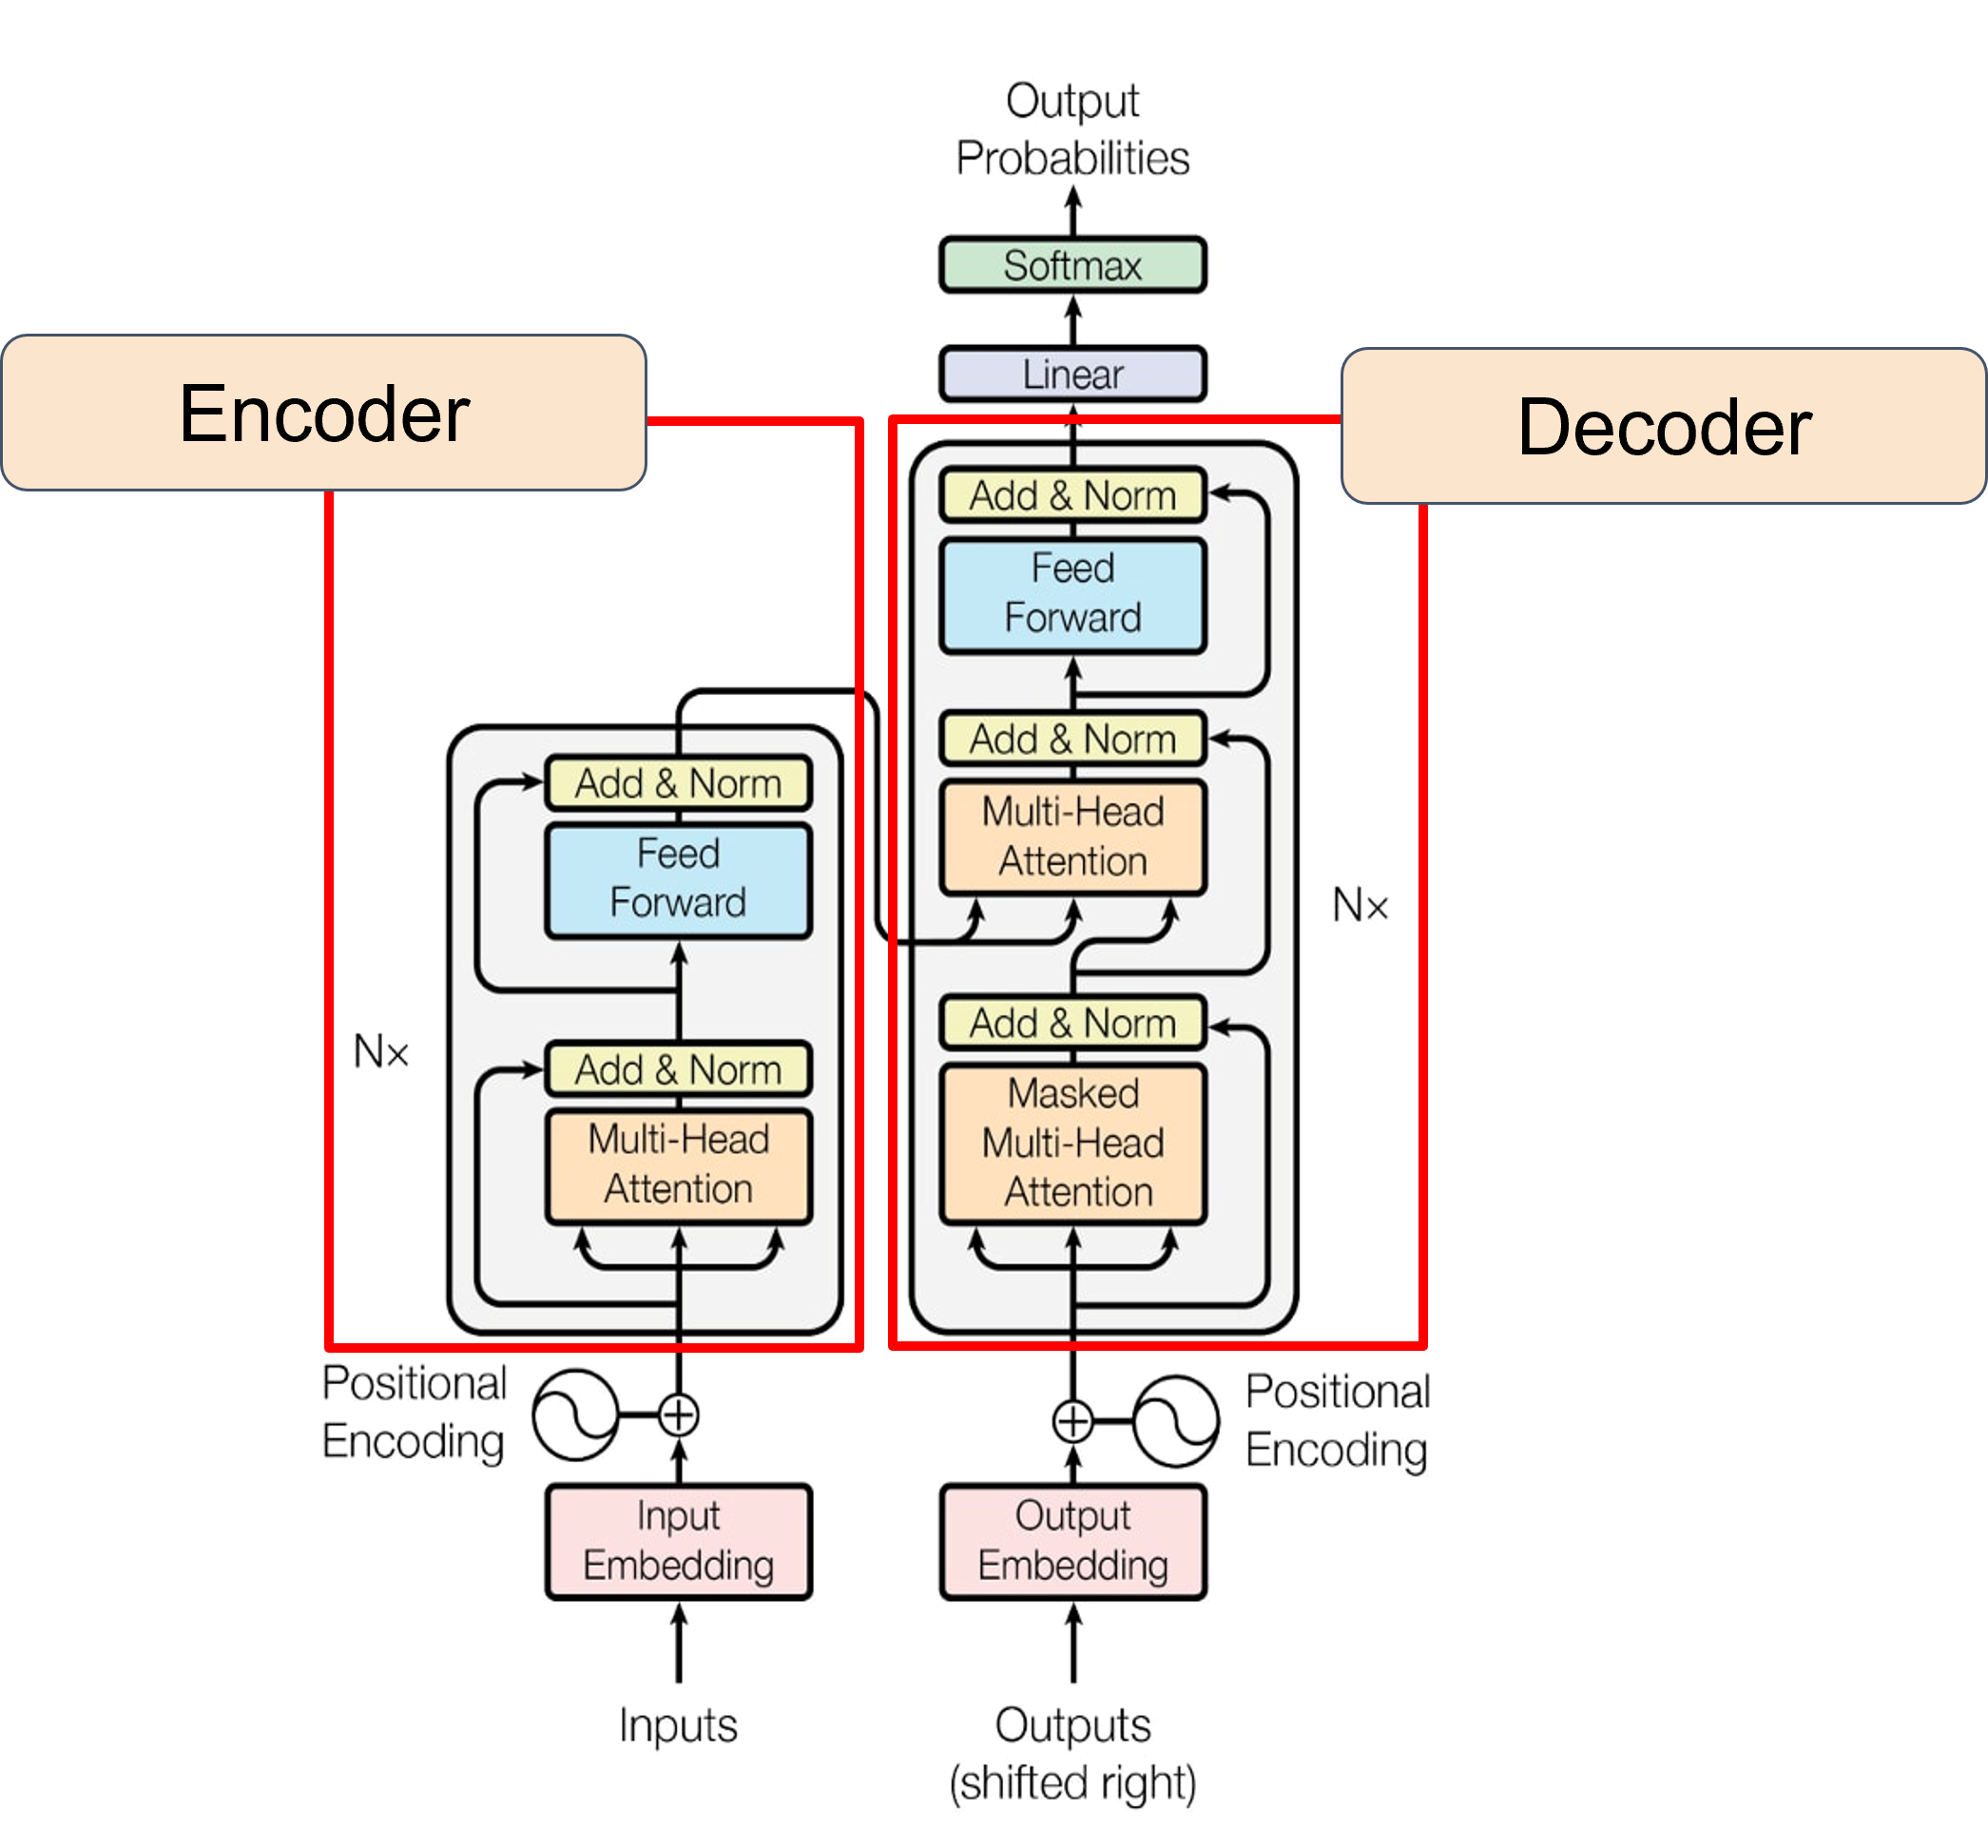
\includegraphics[width=1\linewidth]{Transformer全体像.png}
        \end{figure}
        \column{0.45\textwidth}
        \small
        \begin{itemize}
            \item 左図は, Transformerを構成する最小単位である”ブロック”と呼ばれるもの.
            \item 縦にN層積み重ねてつくる.
            \item 左側：Encoderブロック
            \item 右側：Decoderブロック
        \end{itemize}
    \end{columns}
    \vspace{0.7em}
    \tiny
    \href{https://arxiv.org/abs/1706.03762}{Vaswani, A. et al., Attention Is All You Need, Proceedings of the 31st International Conference on Neural Information Processing Systems, pp.6000 - 6010, 2017.}
\end{frame}

\begin{frame}{モデル構造}
    \framesubtitle{Transformer}
    \vspace{-0.5em}
    \begin{columns}[c]
        \column{0.5\textwidth}
        \begin{figure}[bthp]
        \centering
        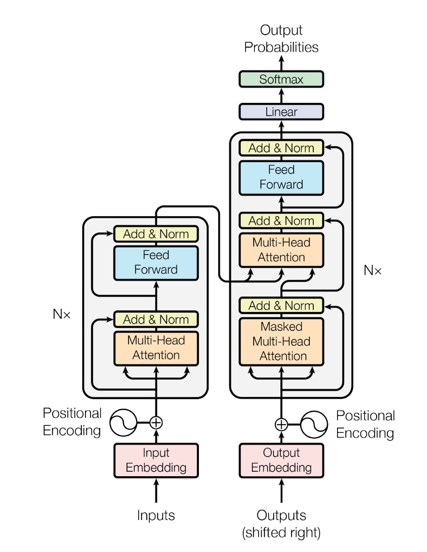
\includegraphics[width=1\linewidth]{Transformer.png}
        \end{figure}
        \column{0.45\textwidth}
        \small
        \begin{itemize}
            \item Embedding
            \item Multi-Head Attention
            \item Feed Forward
            \item Others
        \end{itemize}
        \vspace{0.7em}
        \tiny
        \href{https://arxiv.org/abs/1706.03762}{Vaswani, A. et al., Attention Is All You Need, Proceedings of the 31st International Conference on Neural Information Processing Systems, pp.6000 - 6010, 2017.}
    \end{columns}
\end{frame}

\begin{frame}{モデル構造 - Embedding}
    \framesubtitle{Transformer}
    \vspace{-0.5em}
    \begin{columns}[c]
        \column{0.5\textwidth}
        \begin{figure}[bthp]
        \centering
        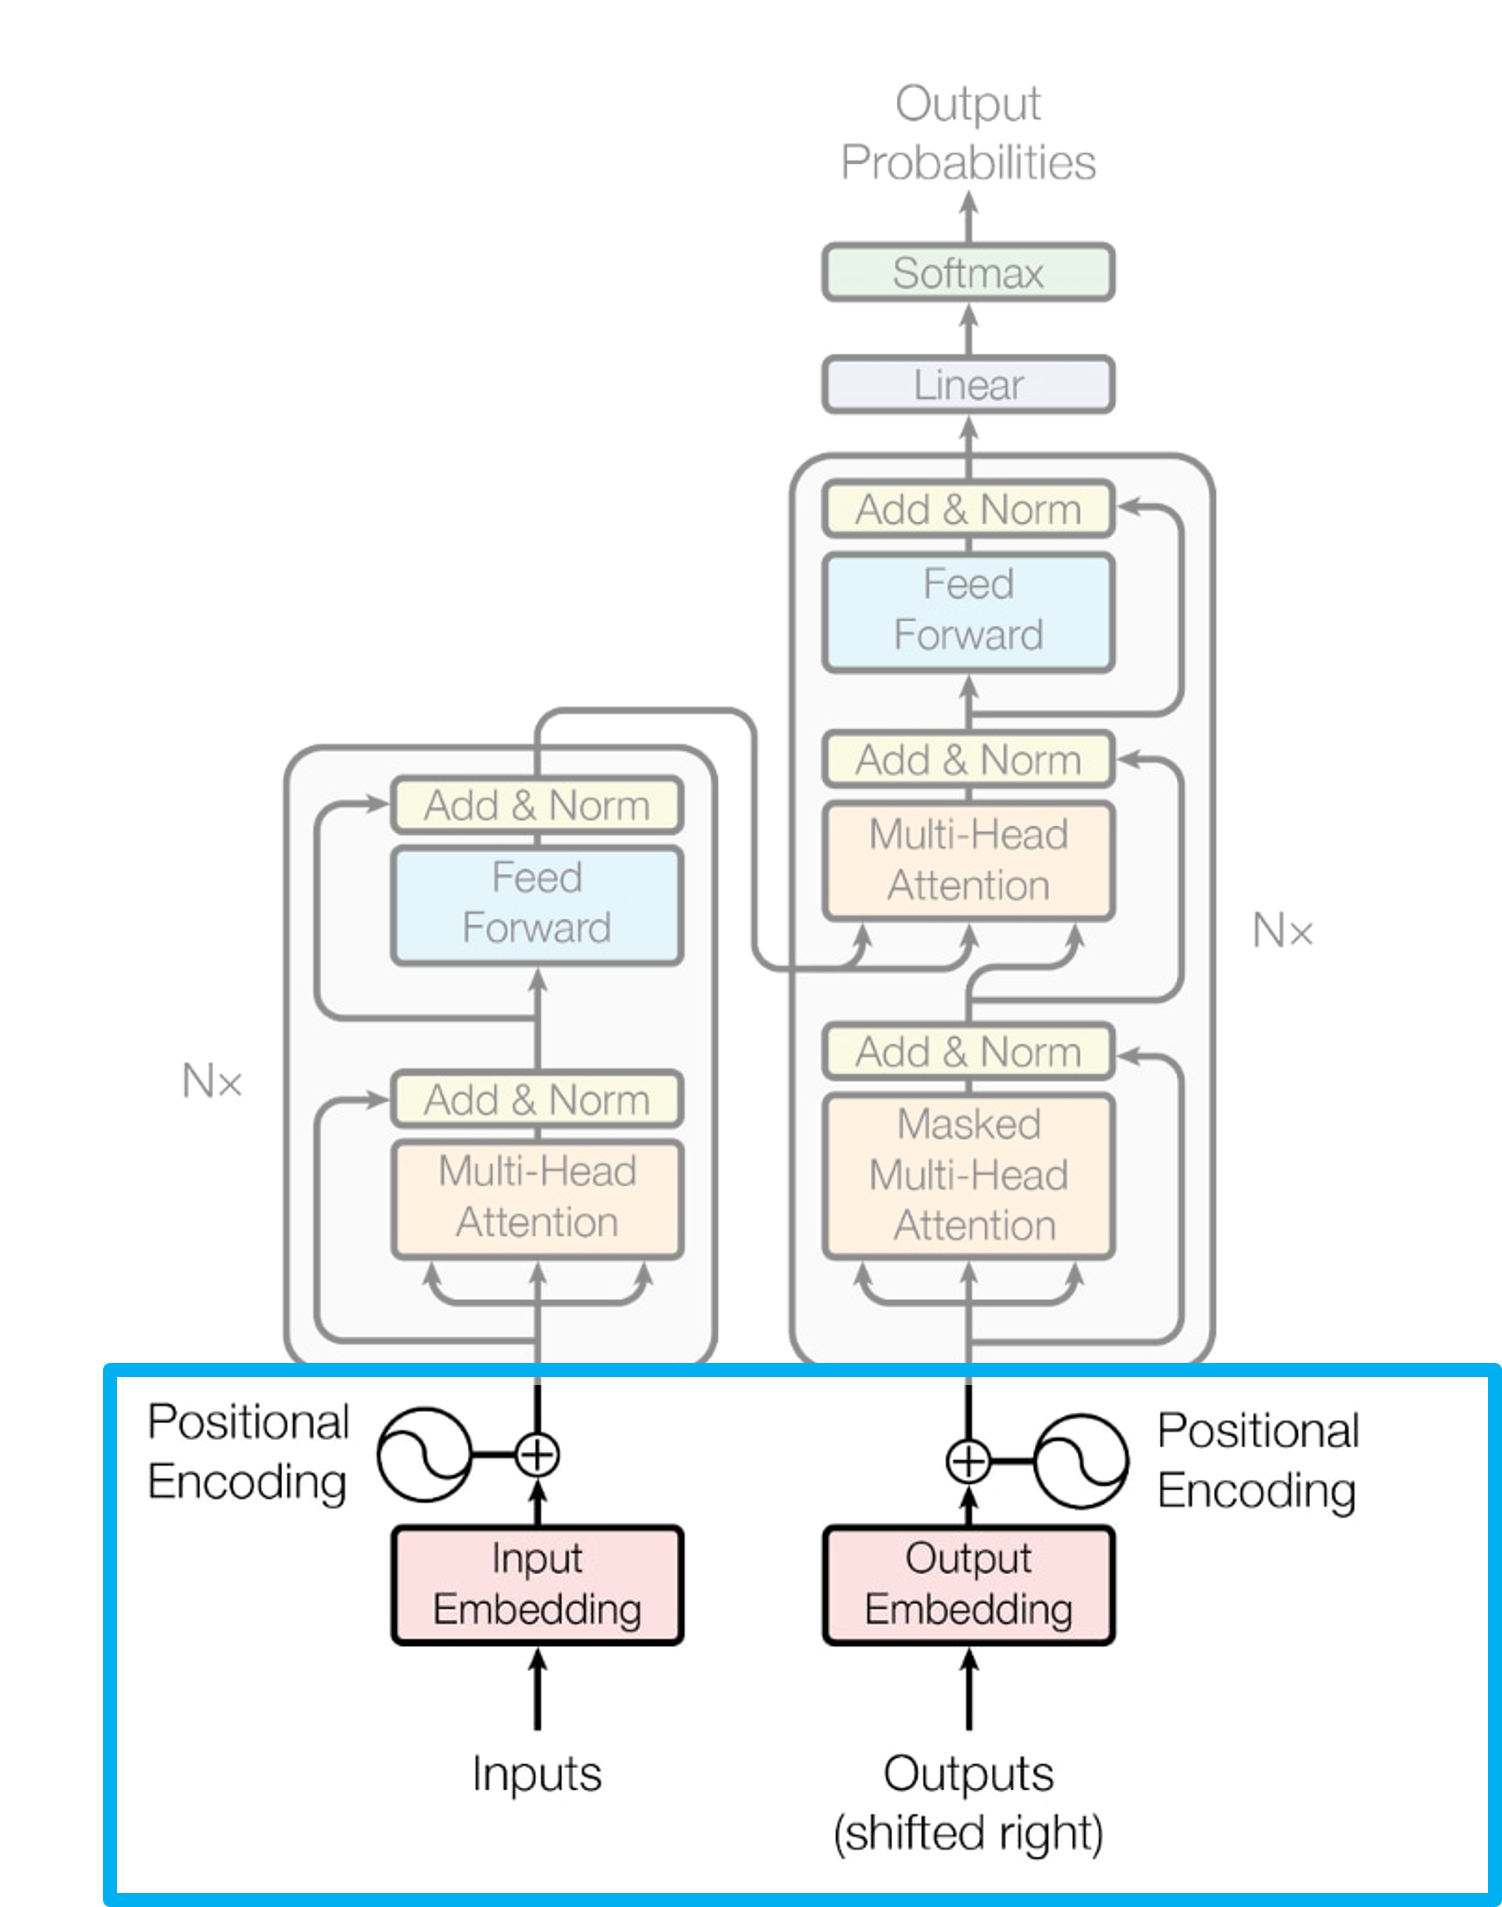
\includegraphics[width=1\linewidth]{Transformer_Embedding.png}
        \end{figure}
        \column{0.45\textwidth}
        \small
        \begin{itemize}
            \item \textcolor{cyan}{Embedding}
            \item Multi-Head Attention
            \item Feed Forward
            \item Others
        \end{itemize}
        \vspace{0.7em}
        \tiny
        \href{https://arxiv.org/abs/1706.03762}{Vaswani, A. et al., Attention Is All You Need, Proceedings of the 31st International Conference on Neural Information Processing Systems, pp.6000 - 6010, 2017.}
    \end{columns}
\end{frame}

\begin{frame}{Word Embedding (WE)}
    \begin{columns}[c]
        \column{0.5\textwidth}
        \begin{figure}[bthp]
            \centering
            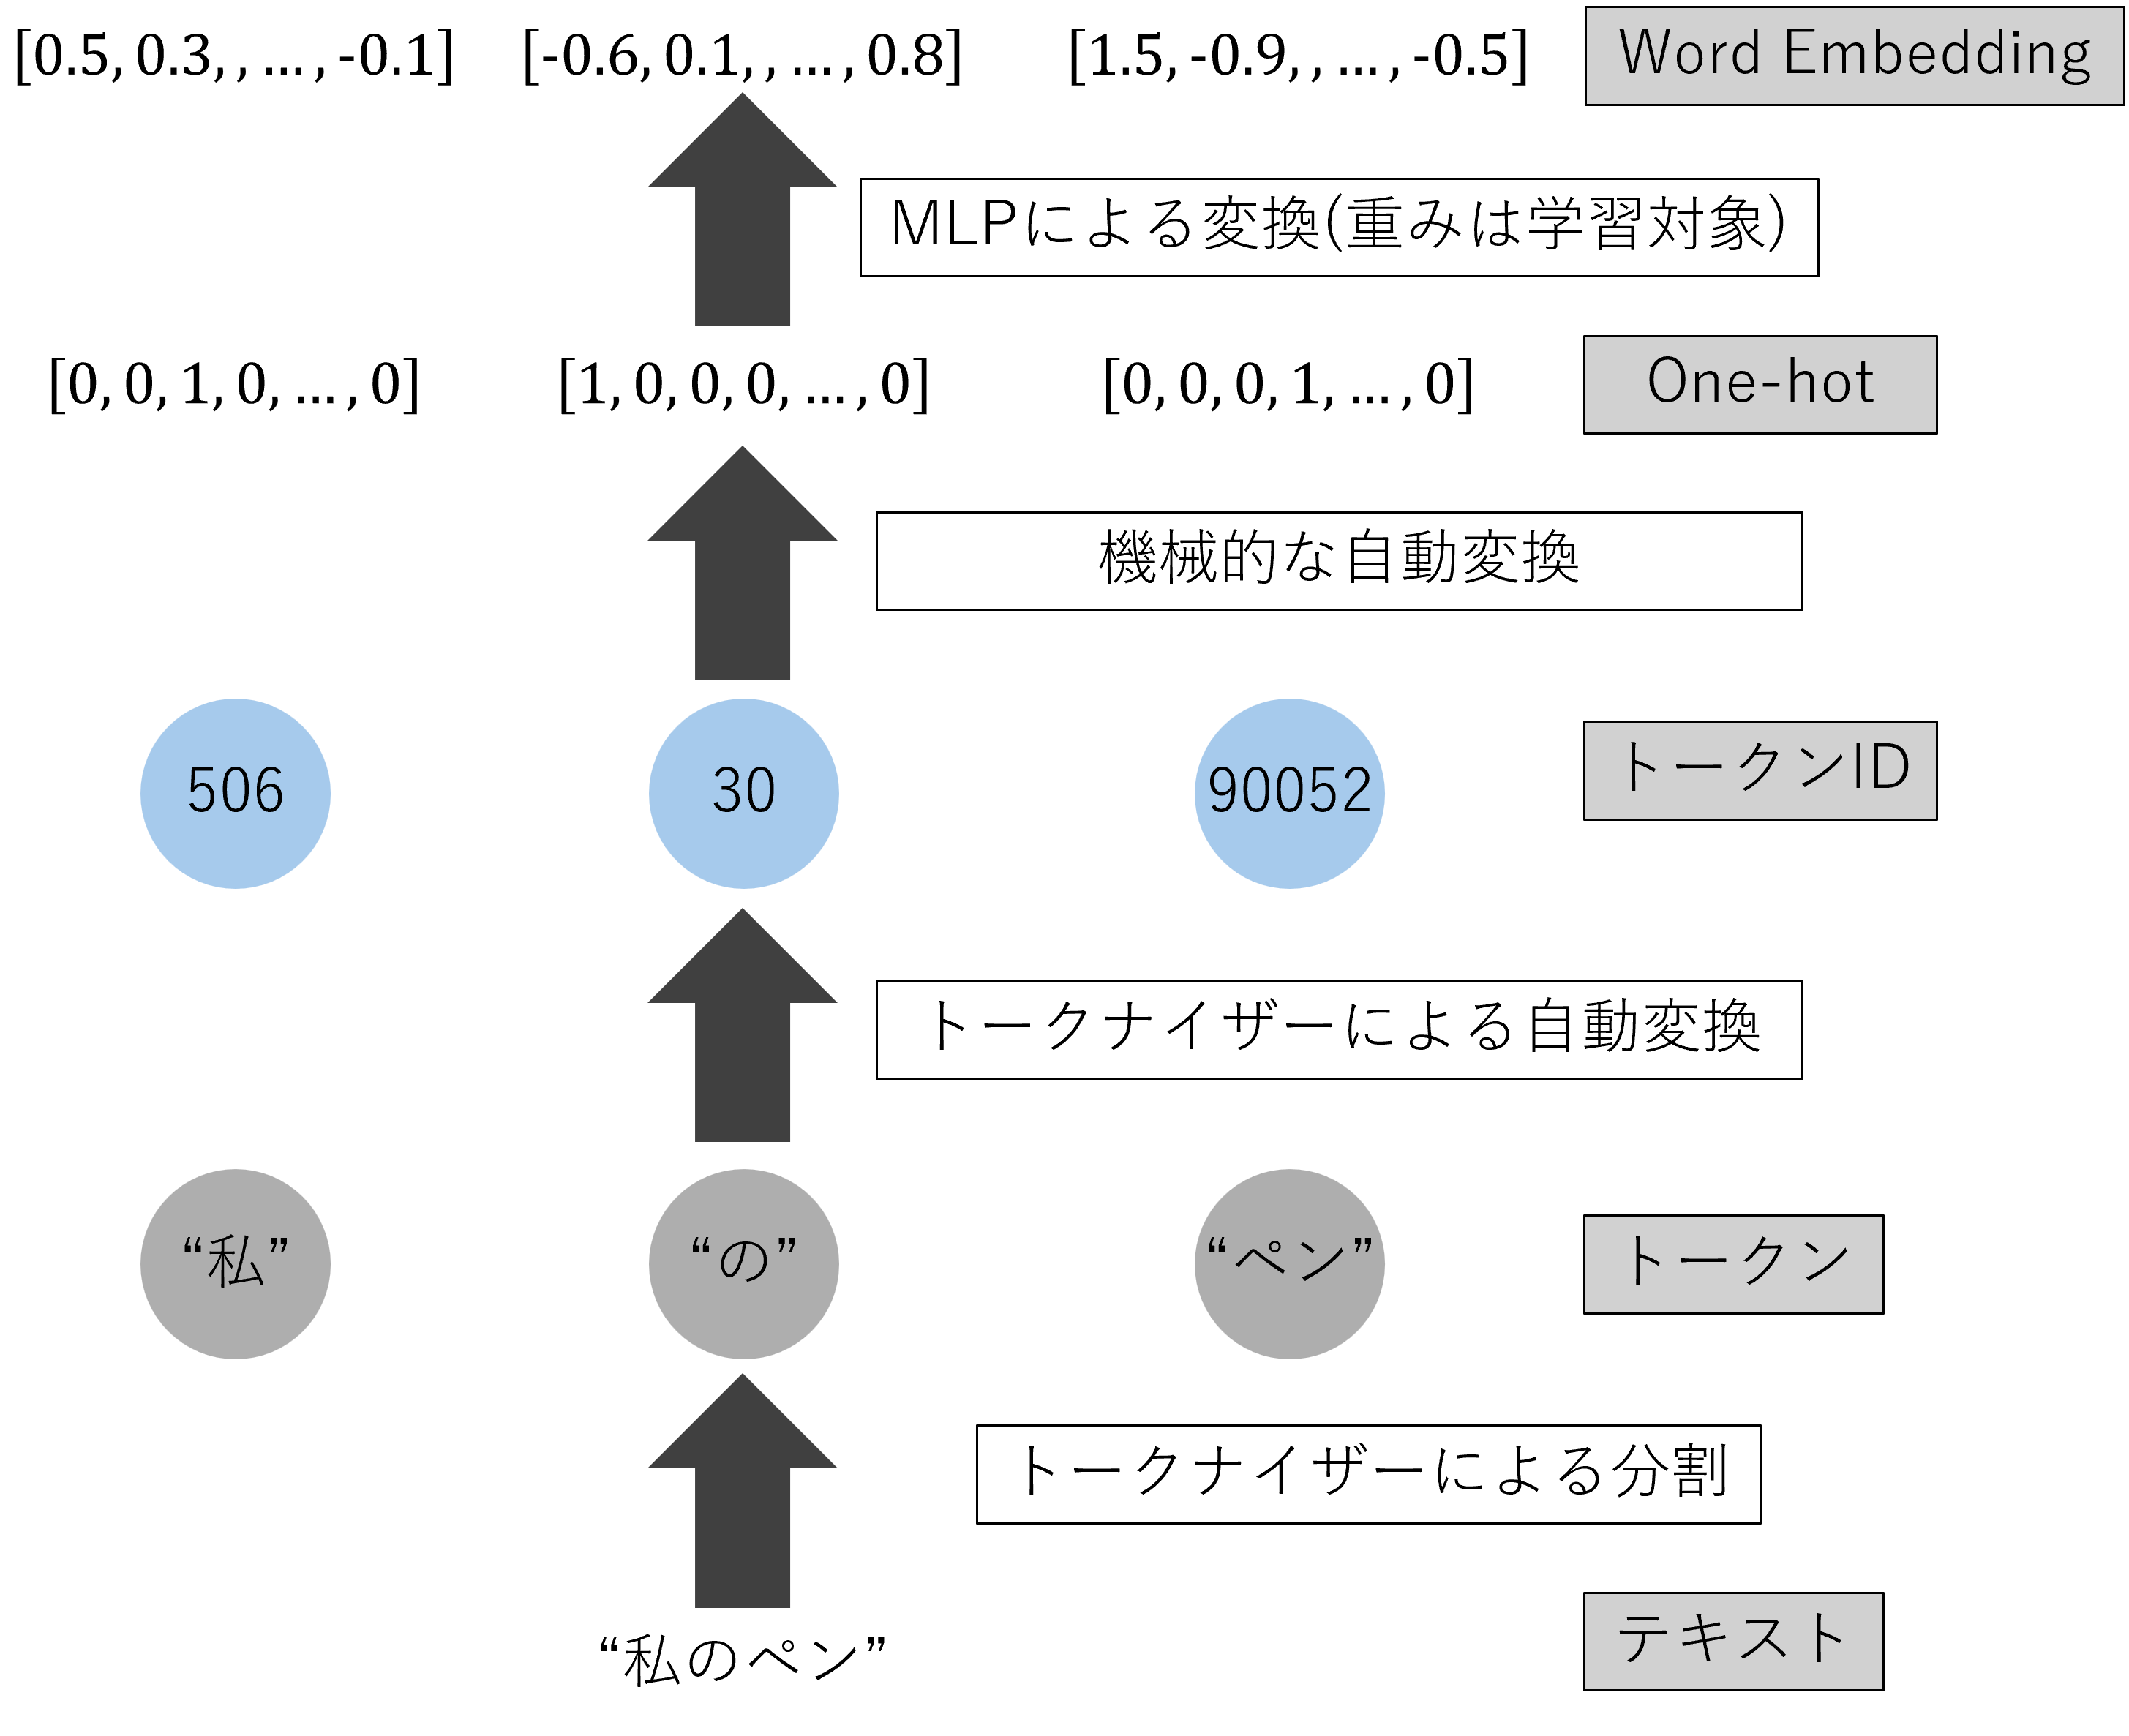
\includegraphics[width=1\linewidth]{Embeddingの流れ.png}
        \end{figure}
        \column{0.4\textwidth}
        \tiny
        総トークン数をVとして、V次元のOne-hotベクトルを埋め込みに変換する行列Eを定義
        \begin{align*}
            E \in \mathbb{R}^{V \times d_{\text{model}}}
        \end{align*}
        t=[0,0..,1,..,0,0]を,第k成分のみ1で、他は全て0のOne-hotベクトルとする
        \begin{align*}
            tE = d
        \end{align*}
        \bm{d}はEのk行目と一致する横ベクトル
    \end{columns}
    \vspace{1.5em}
    \tiny
    \href{https://arxiv.org/abs/1706.03762}{Vaswani, A. et al., Attention Is All You Need, Proceedings of the 31st International Conference on Neural Information Processing Systems, pp.6000 - 6010, 2017.}
\end{frame}

\begin{frame}{Positional Encoding(PE)}
    \begin{figure}[bthp]
    \centering
    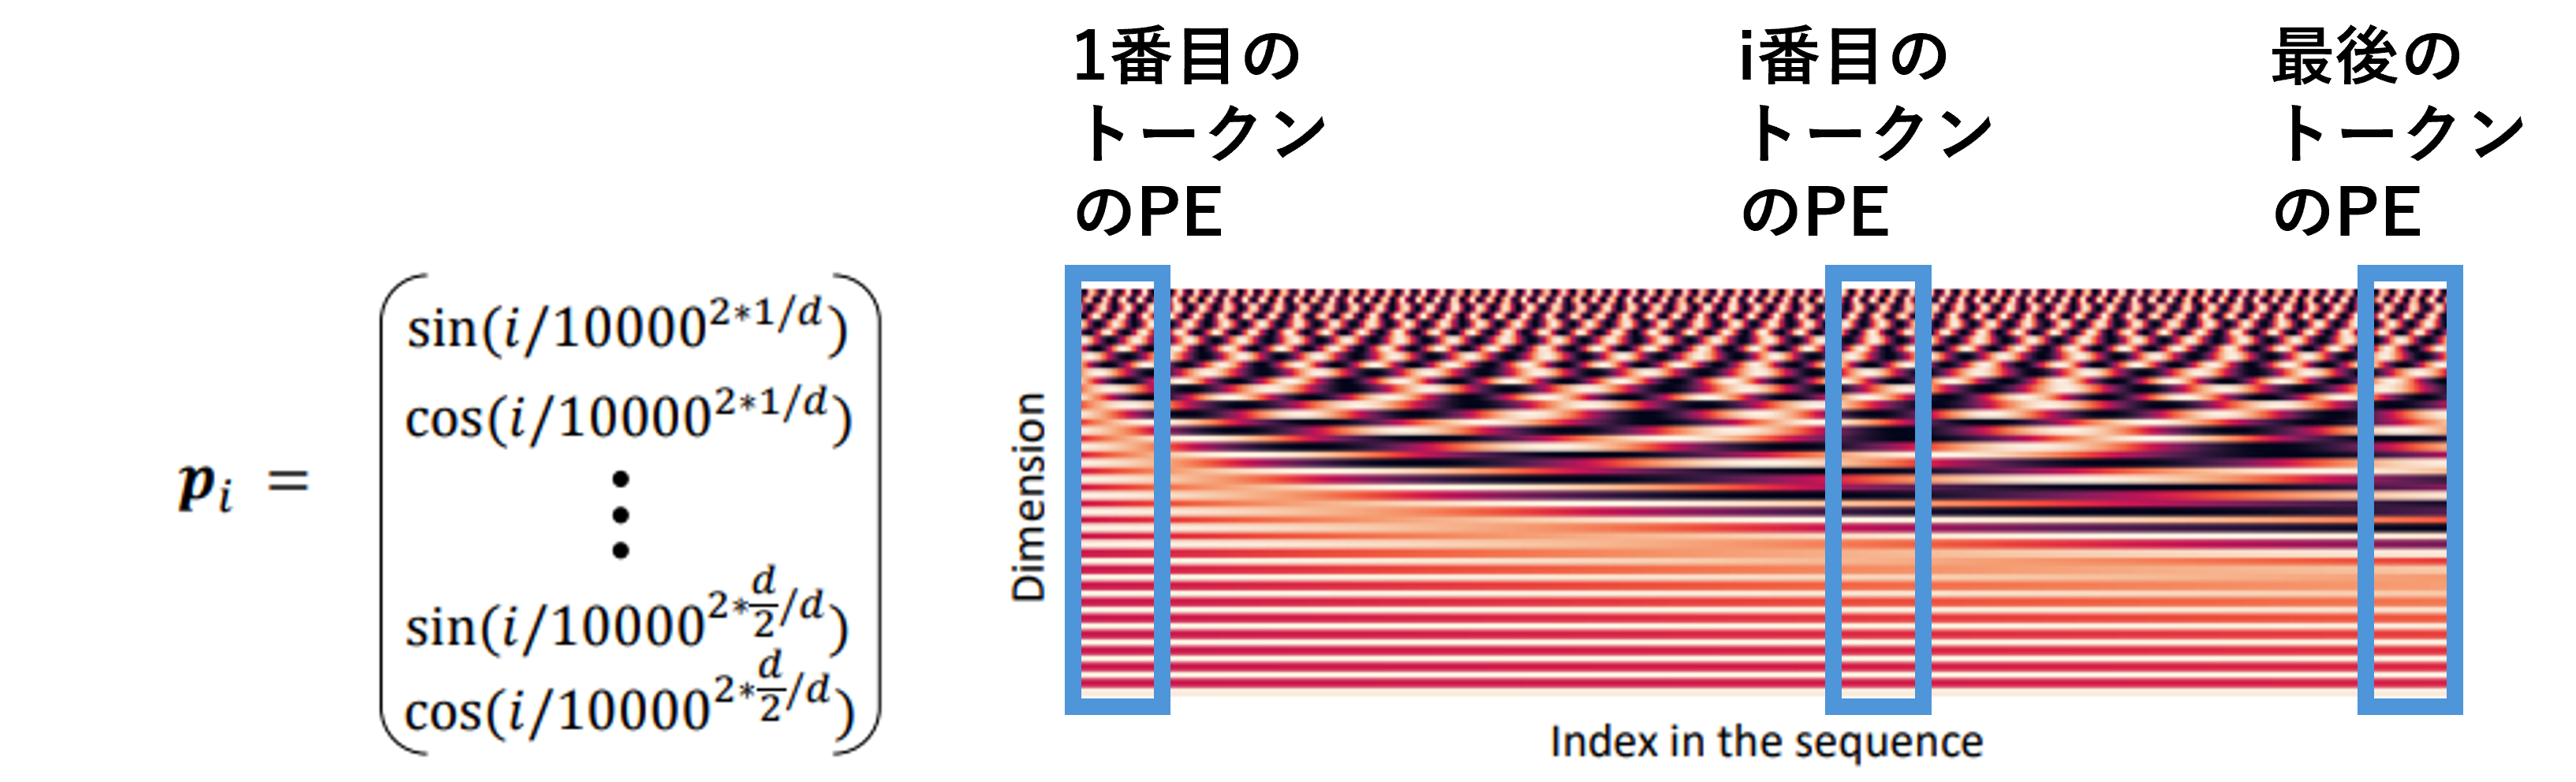
\includegraphics[width=1\linewidth]{Positional Encoding_image.png}
    \end{figure}
    \begin{columns}[c]
        \column{0.45\textwidth}
        \tiny
        \begin{itemize}
            \item $p_i$ : i番目のトークンのPE
            \item $d$ : 特徴量$d_{model}$の次元数
        \end{itemize}
        \column{0.45\textwidth}
        \tiny
        Transformerブロックは単語の位置情報を把握できないため, \textcolor{red}{Word Embeddingに位置情報(PE)を加算.}
    \end{columns}
    \vspace{2em}
    \tiny
    \href{https://arxiv.org/abs/1706.03762}{Vaswani, A. et al., Attention Is All You Need, Proceedings of the 31st International Conference on Neural Information Processing Systems, pp.6000 - 6010, 2017.}
    
    \href{https://web.stanford.edu/class/archive/cs/cs224n/cs224n.1234/slides/cs224n-2023-lecture08-transformers.pdf}{John Hewitt, Natural Language Processing with Deep Learning CS224N/Ling284}
\end{frame}

\begin{frame}{モデル構造 - Multi-head Attention}
    \framesubtitle{Transformer}
    \vspace{-0.5em}
    \begin{columns}[c]
        \column{0.5\textwidth}
        \begin{figure}[bthp]
        \centering
        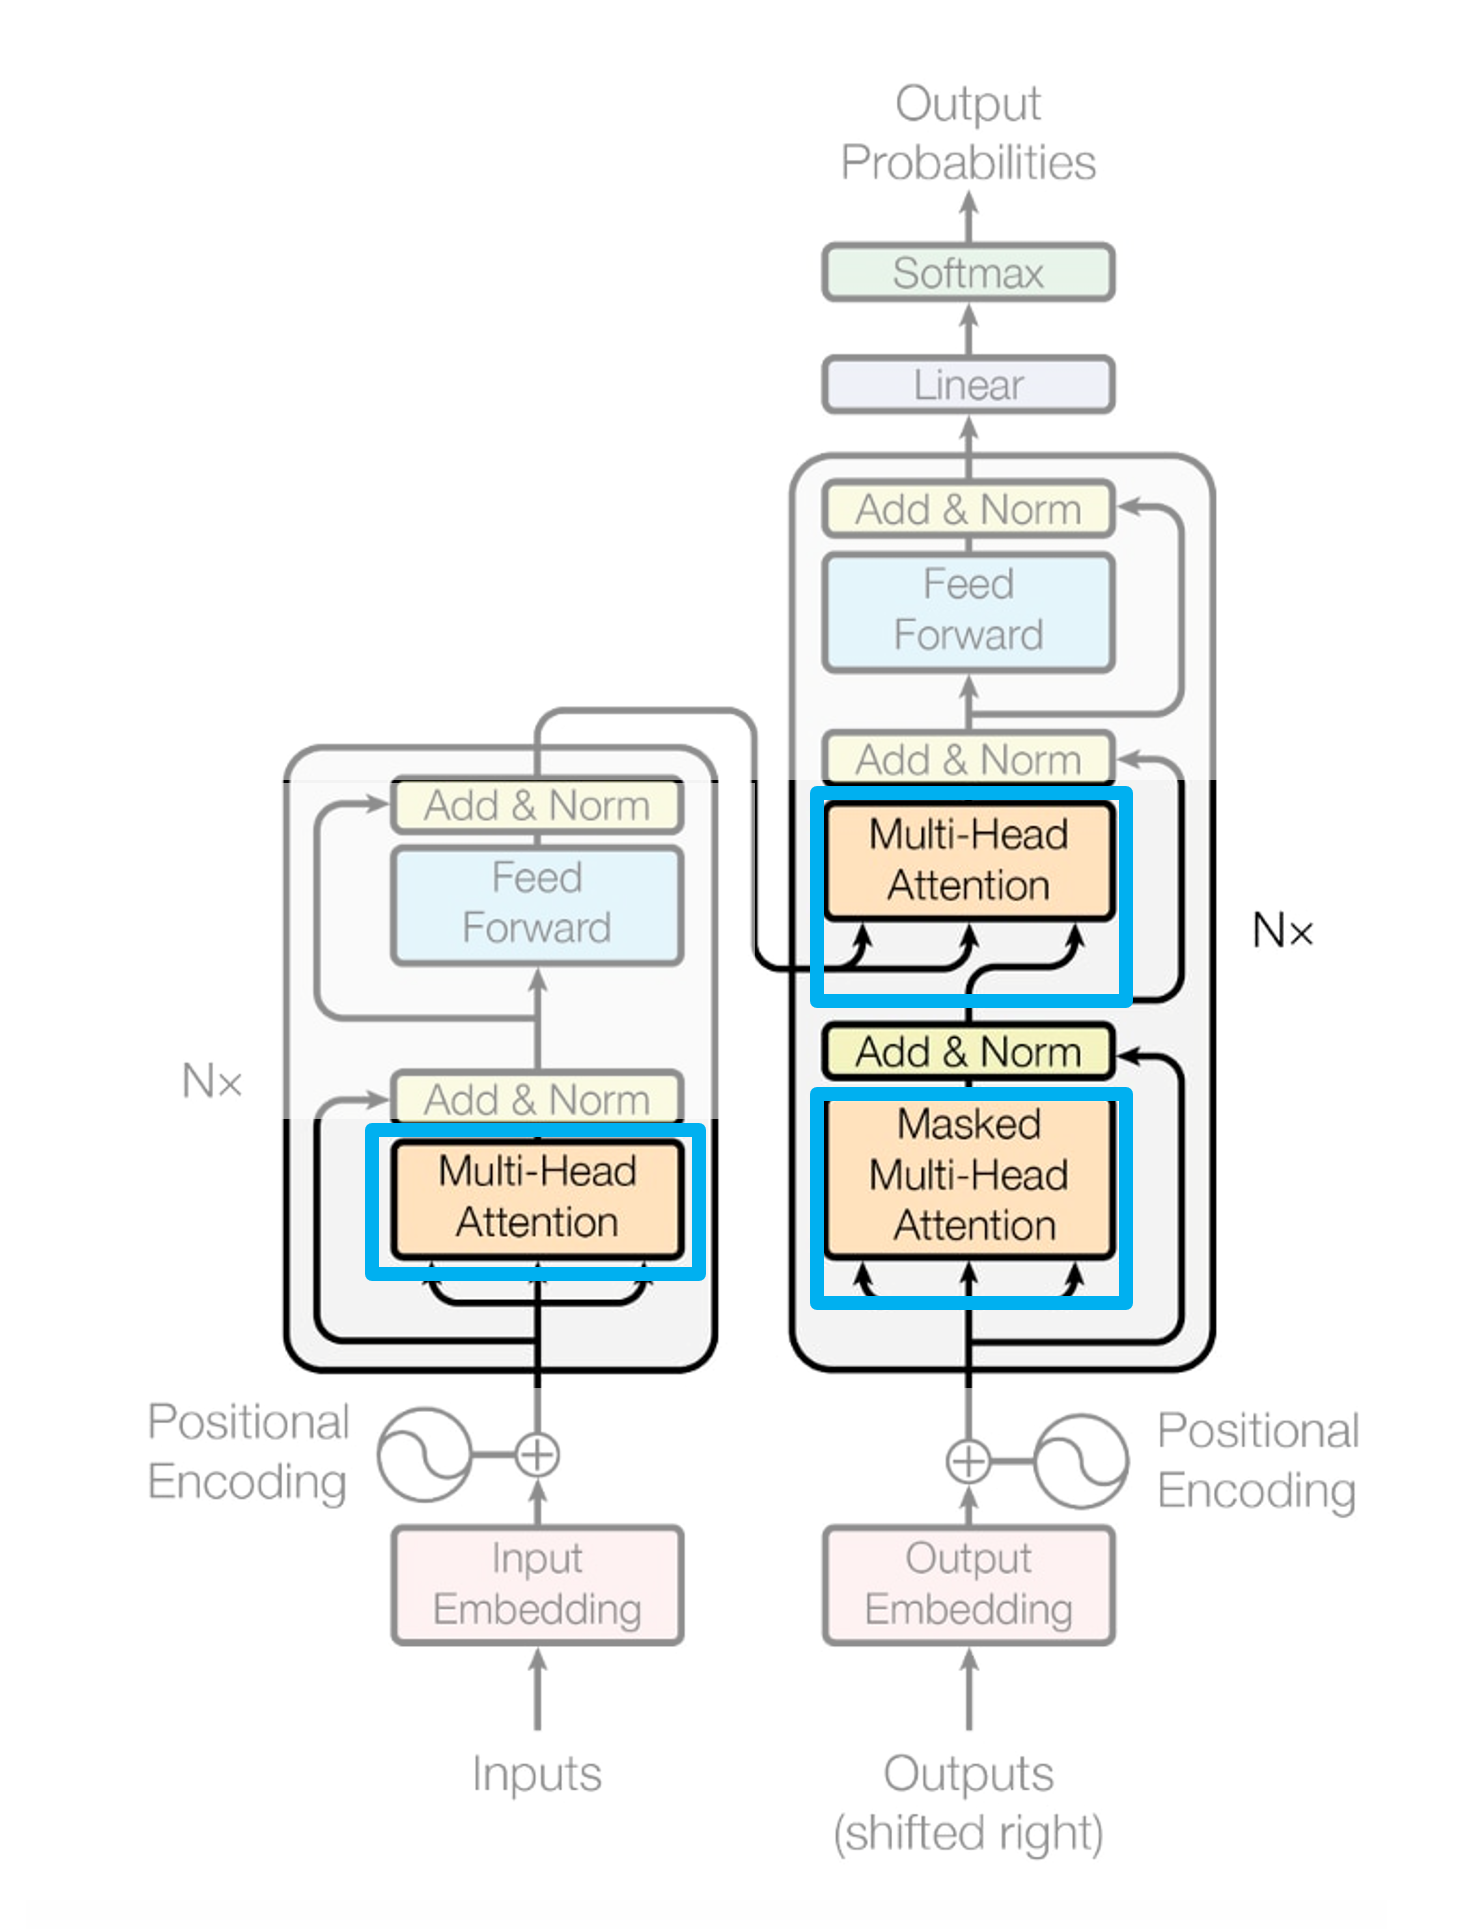
\includegraphics[width=1\linewidth]{Transformer_MultiheadAttention.png}
        \end{figure}
        \column{0.45\textwidth}
        \small
        \begin{itemize}
            \item Embedding
            \item \textcolor{cyan}{Multi-Head Attention}
            \item Feed Forward
            \item Others
        \end{itemize}
        \vspace{0.7em}
        \tiny
        \href{https://arxiv.org/abs/1706.03762}{Vaswani, A. et al., Attention Is All You Need, Proceedings of the 31st International Conference on Neural Information Processing Systems, pp.6000 - 6010, 2017.}
    \end{columns}
\end{frame}

\begin{frame}{Scaled Dot-Product Attention}
    \begin{columns}[T]
        \vspace{-1em}
        \column{0.3\textwidth}
        \begin{figure}[bthp]
        \centering
        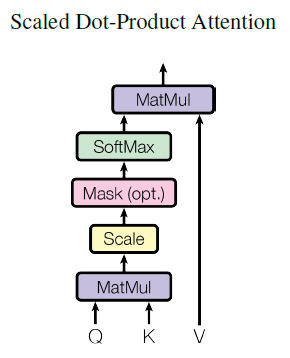
\includegraphics[width=0.9\linewidth]{Scaled Dot Product Attention.png}
        \end{figure}
        \vspace{-1em}
        \begin{table}[]
            \tiny
            \begin{tabular}{lll}
                \hline
                \textbf{変数} & \textbf{名称} & \textbf{イメージ・定義} \\ \hline
                $Q\in \mathbb{R}^{n \times d_{k}}$ & Query &  「何に注目したいか」 \\
                $K\in \mathbb{R}^{n \times d_{k}}$ & Key & 「どのような情報を持っているか」 \\
                $V\in \mathbb{R}^{n \times d_{v}}$ & Value & 実際に抽出される「情報」 \\
                $n$ & シーケンス長 & 入力トークン数 \\
                $d_k$ & 次元数 & $Q, K$ の次元数 \\
                $d_v$ & 次元数 & $V$ の次元数 \\
                $\text{softmax}$ & 関数 & 正規化する処理 \\ \hline
            \end{tabular}
        \end{table}
        \column{0.5\textwidth}
        \tiny
        \[
        \text{Attention}(Q, K, V) = \text{softmax}\left(\frac{QK^\top}{\sqrt{d_k}}\right)V
        \]
        \vspace{0.5em}
        {\tiny \textbf{処理フロー}}
        \begin{itemize}
            \item \textbf{1. MatMul}: $Q$と$K$の内積により単語間の相関（スコア）を算出
            \item \textbf{2. Scale}: $\sqrt{d_k}$で除算。$d_k$増大による勾配消失を防止
            \item \textbf{3. Softmax}: スコアを合計1の確率（重み）に正規化
            \item \textbf{4. MatMul}: 重みに基づき$V$を足し合わせ、文脈を集約
        \end{itemize}
    \end{columns}
    \vspace{0.5em}
    \tiny
    \href{https://arxiv.org/abs/1706.03762}{Vaswani, A. et al., Attention Is All You Need, Proceedings of the 31st International Conference on Neural Information Processing Systems, pp.6000 - 6010, 2017.}
\end{frame}

\begin{frame}{Scaled Dot-Product Attention 1}
    \begin{figure}[bthp]
        \centering
        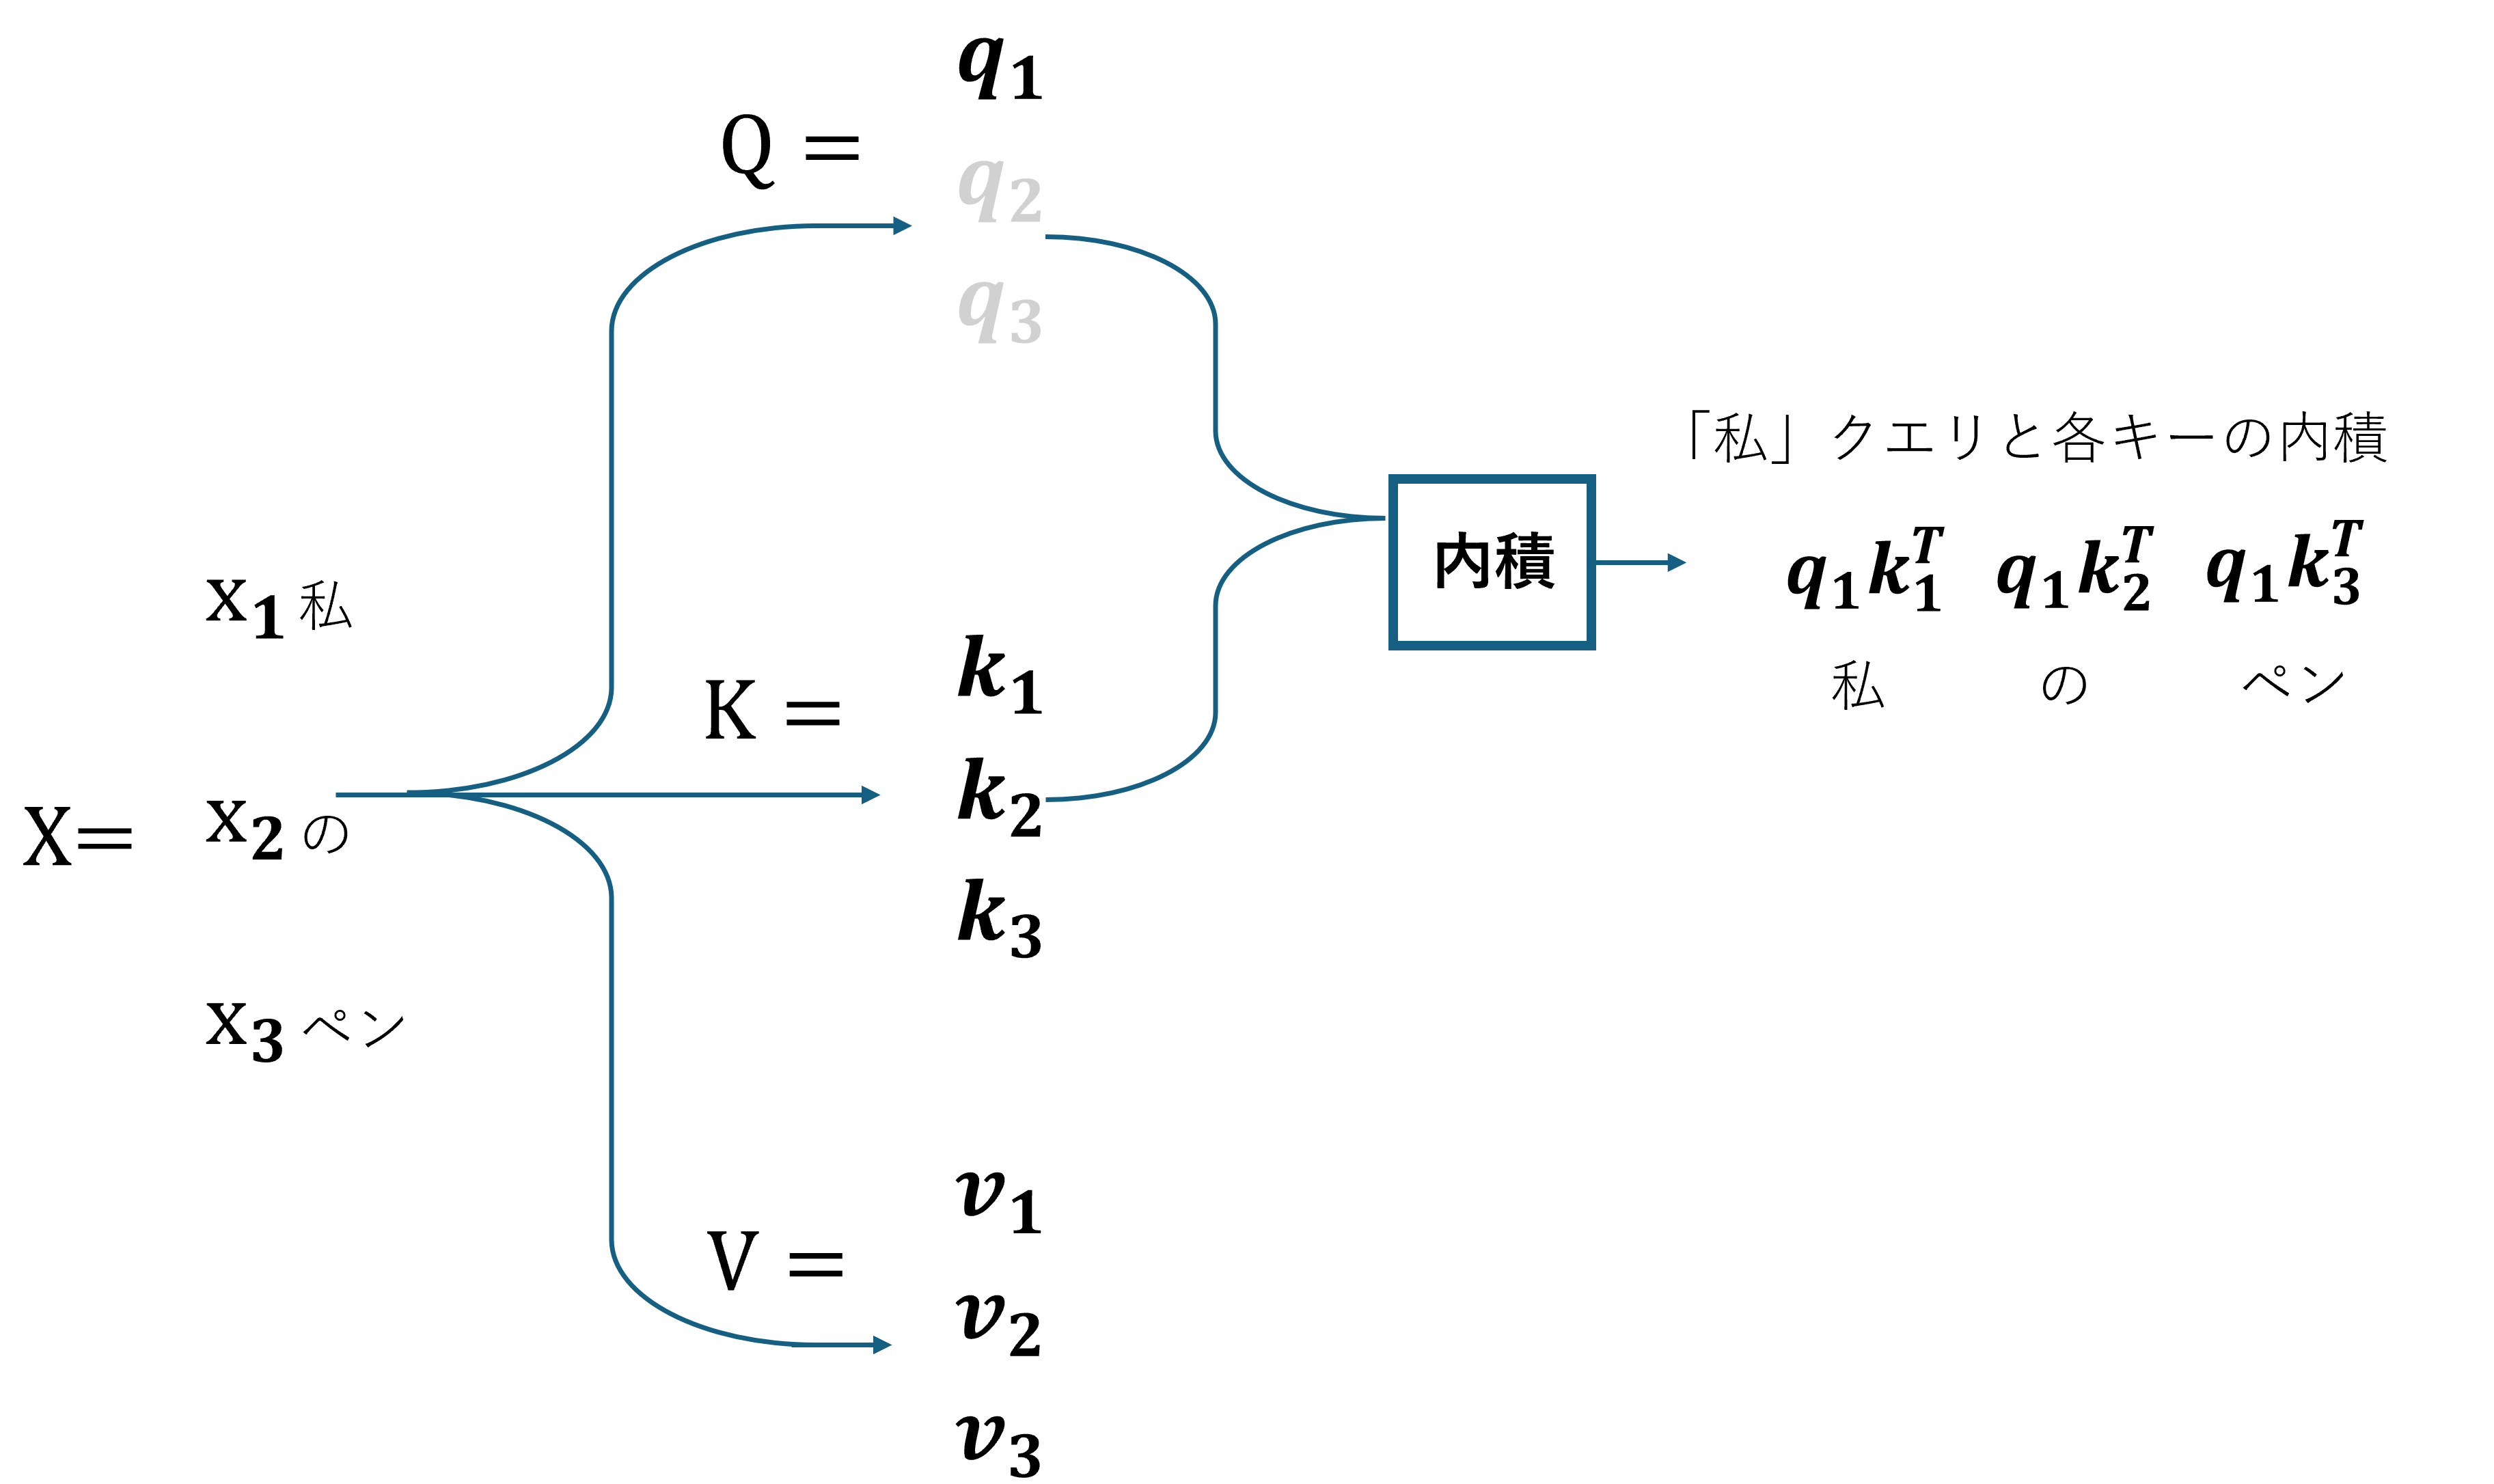
\includegraphics[width=0.8\linewidth]{Scaled Dot 1.png}
    \end{figure}
    \footnotesize
    Query(注目したい単語)と各Key(文中の各単語)がどれだけ関連しているか(類似度)を算出
    
    \vspace{1.5em}
    \tiny
    \href{https://arxiv.org/abs/1706.03762}{Vaswani, A. et al., Attention Is All You Need, Proceedings of the 31st International Conference on Neural Information Processing Systems, pp.6000 - 6010, 2017.}
\end{frame}

\begin{frame}{Scaled Dot-Product Attention 2}
    \begin{figure}[bthp]
        \centering
        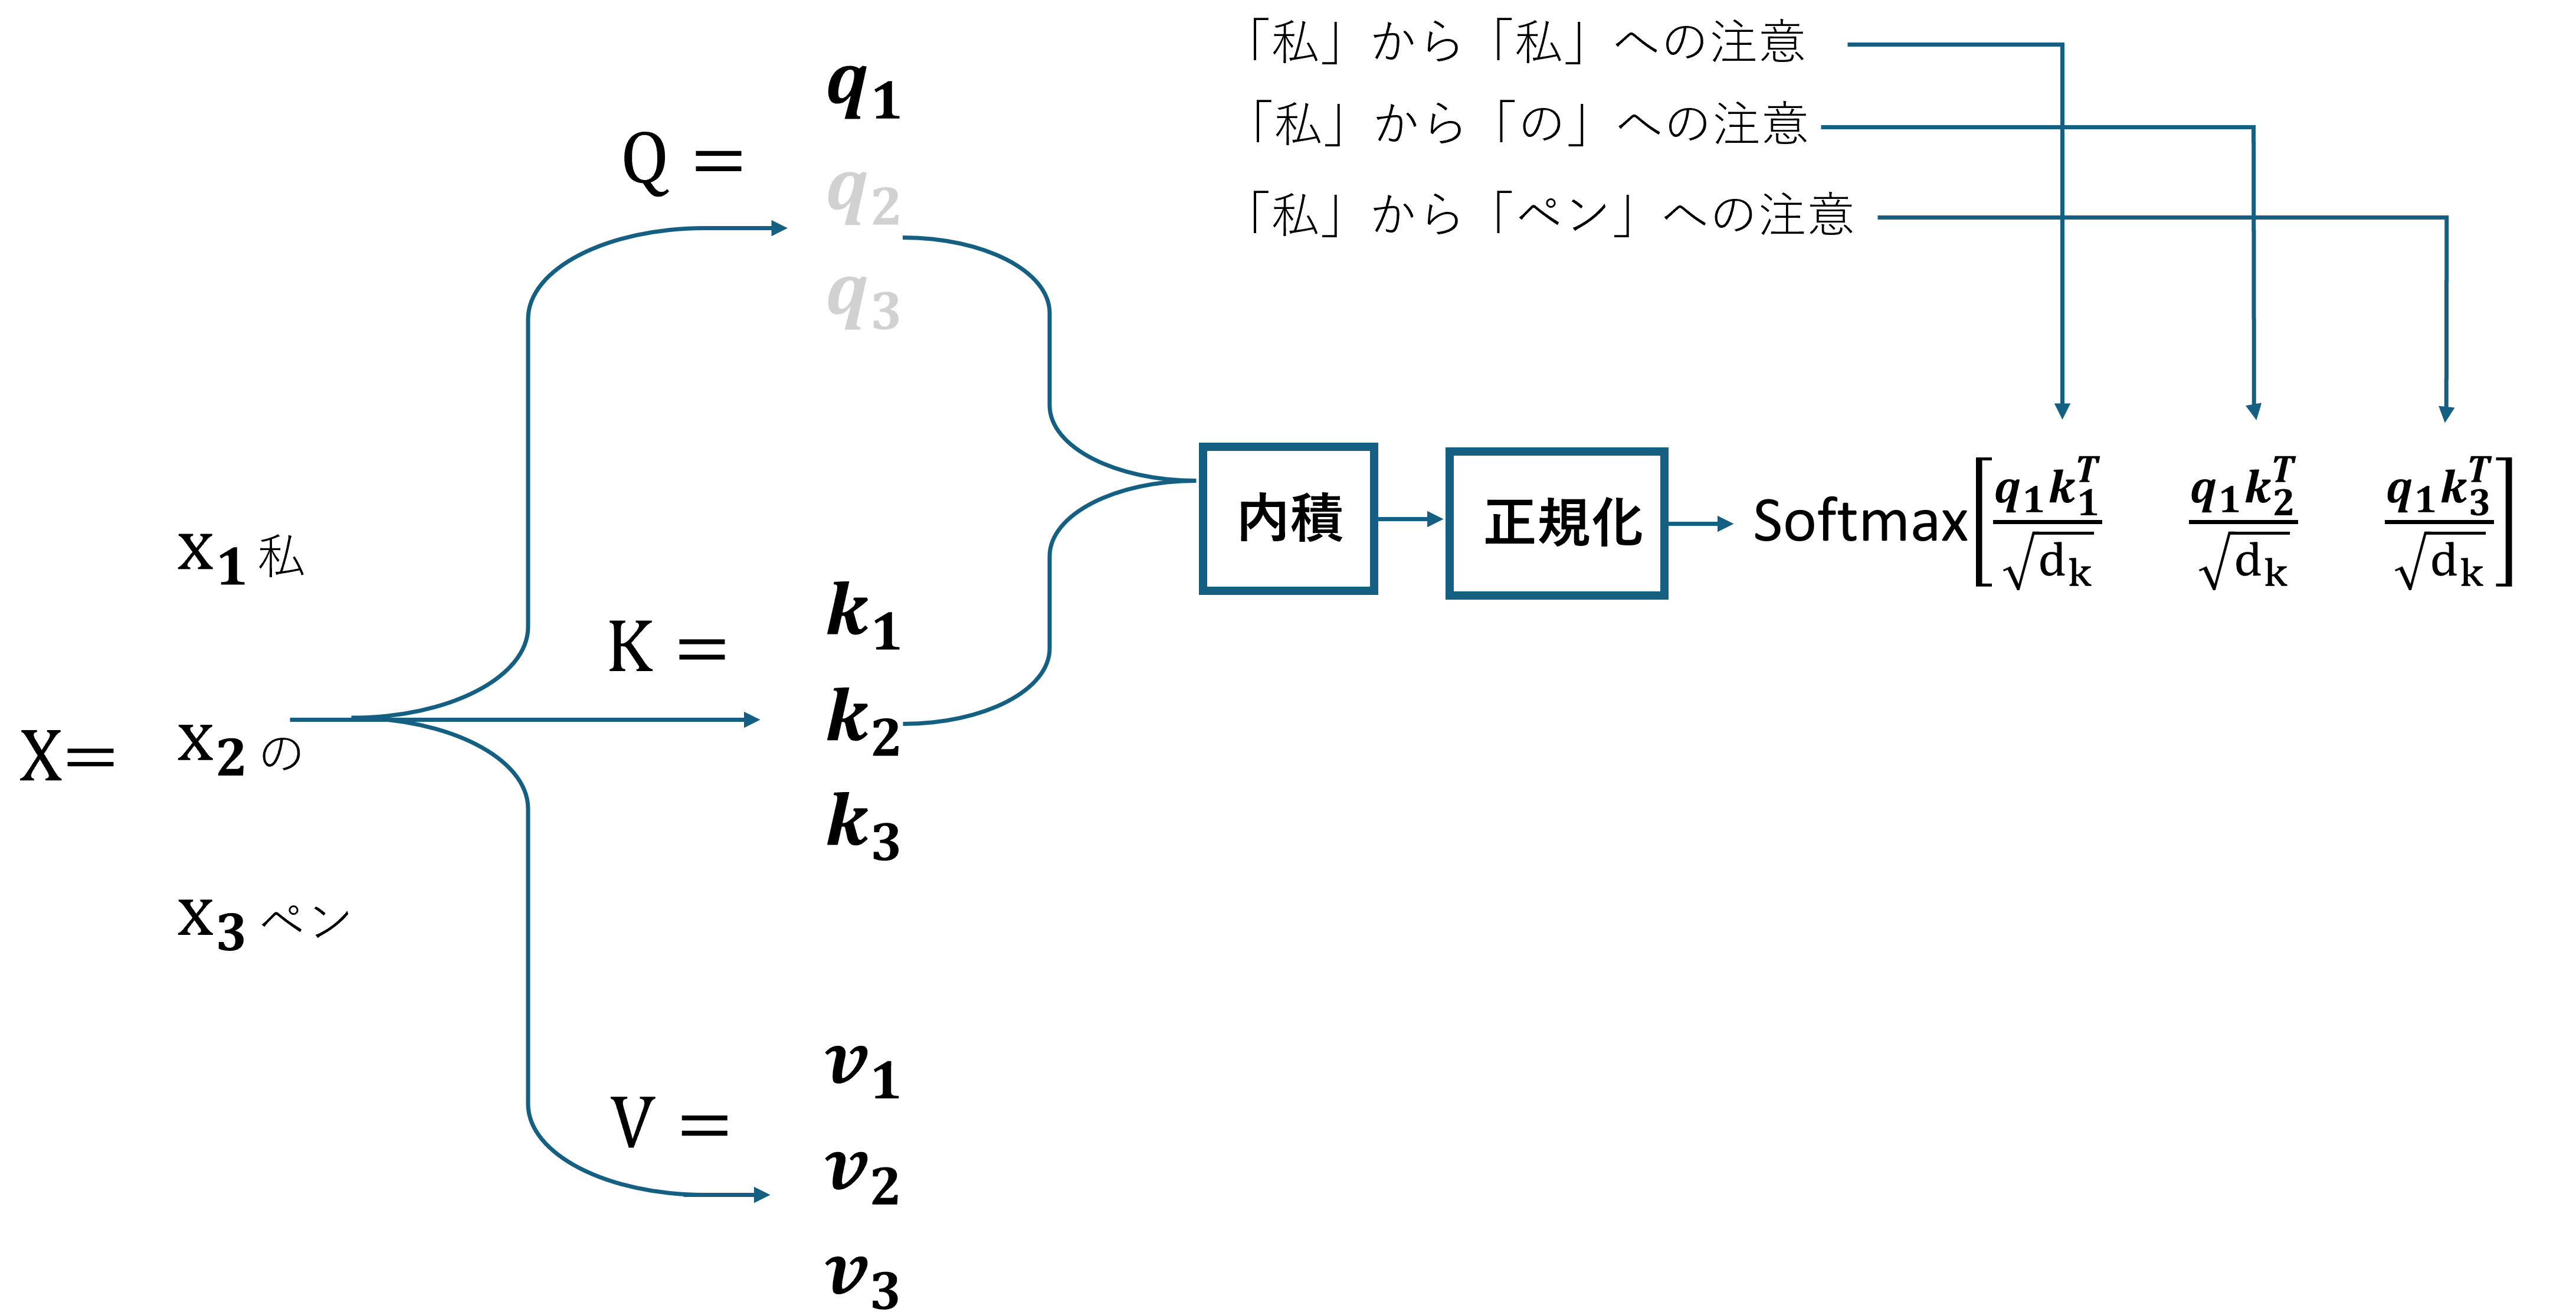
\includegraphics[width=0.8\linewidth]{Scaled Dot 2.png}
    \end{figure}
    \footnotesize
    Queryと各Keyの内積を正規化したものを「対象の単語が周りの各単語をどれほど注視しているか」の指標とみなす(=注意重み)

    \vspace{1.5em}
    \tiny
    \href{https://arxiv.org/abs/1706.03762}{Vaswani, A. et al., Attention Is All You Need, Proceedings of the 31st International Conference on Neural Information Processing Systems, pp.6000 - 6010, 2017.}
\end{frame}

\begin{frame}{Scaled Dot-Product Attention 3}
    \begin{figure}[bthp]
        \centering
        \includegraphics[width=0.8\linewidth]{Scaled Dot 3.png}
    \end{figure}
    \footnotesize
    注意重みで重み付けされたValueの和を計算することで「私」のベクトルに周辺の単語情報が付加される

    \vspace{1.5em}
    \tiny
    \href{https://arxiv.org/abs/1706.03762}{Vaswani, A. et al., Attention Is All You Need, Proceedings of the 31st International Conference on Neural Information Processing Systems, pp.6000 - 6010, 2017.}
\end{frame}

\begin{frame}{Scaled Dot-Product Attention 4}
    \begin{figure}[bthp]
        \centering
        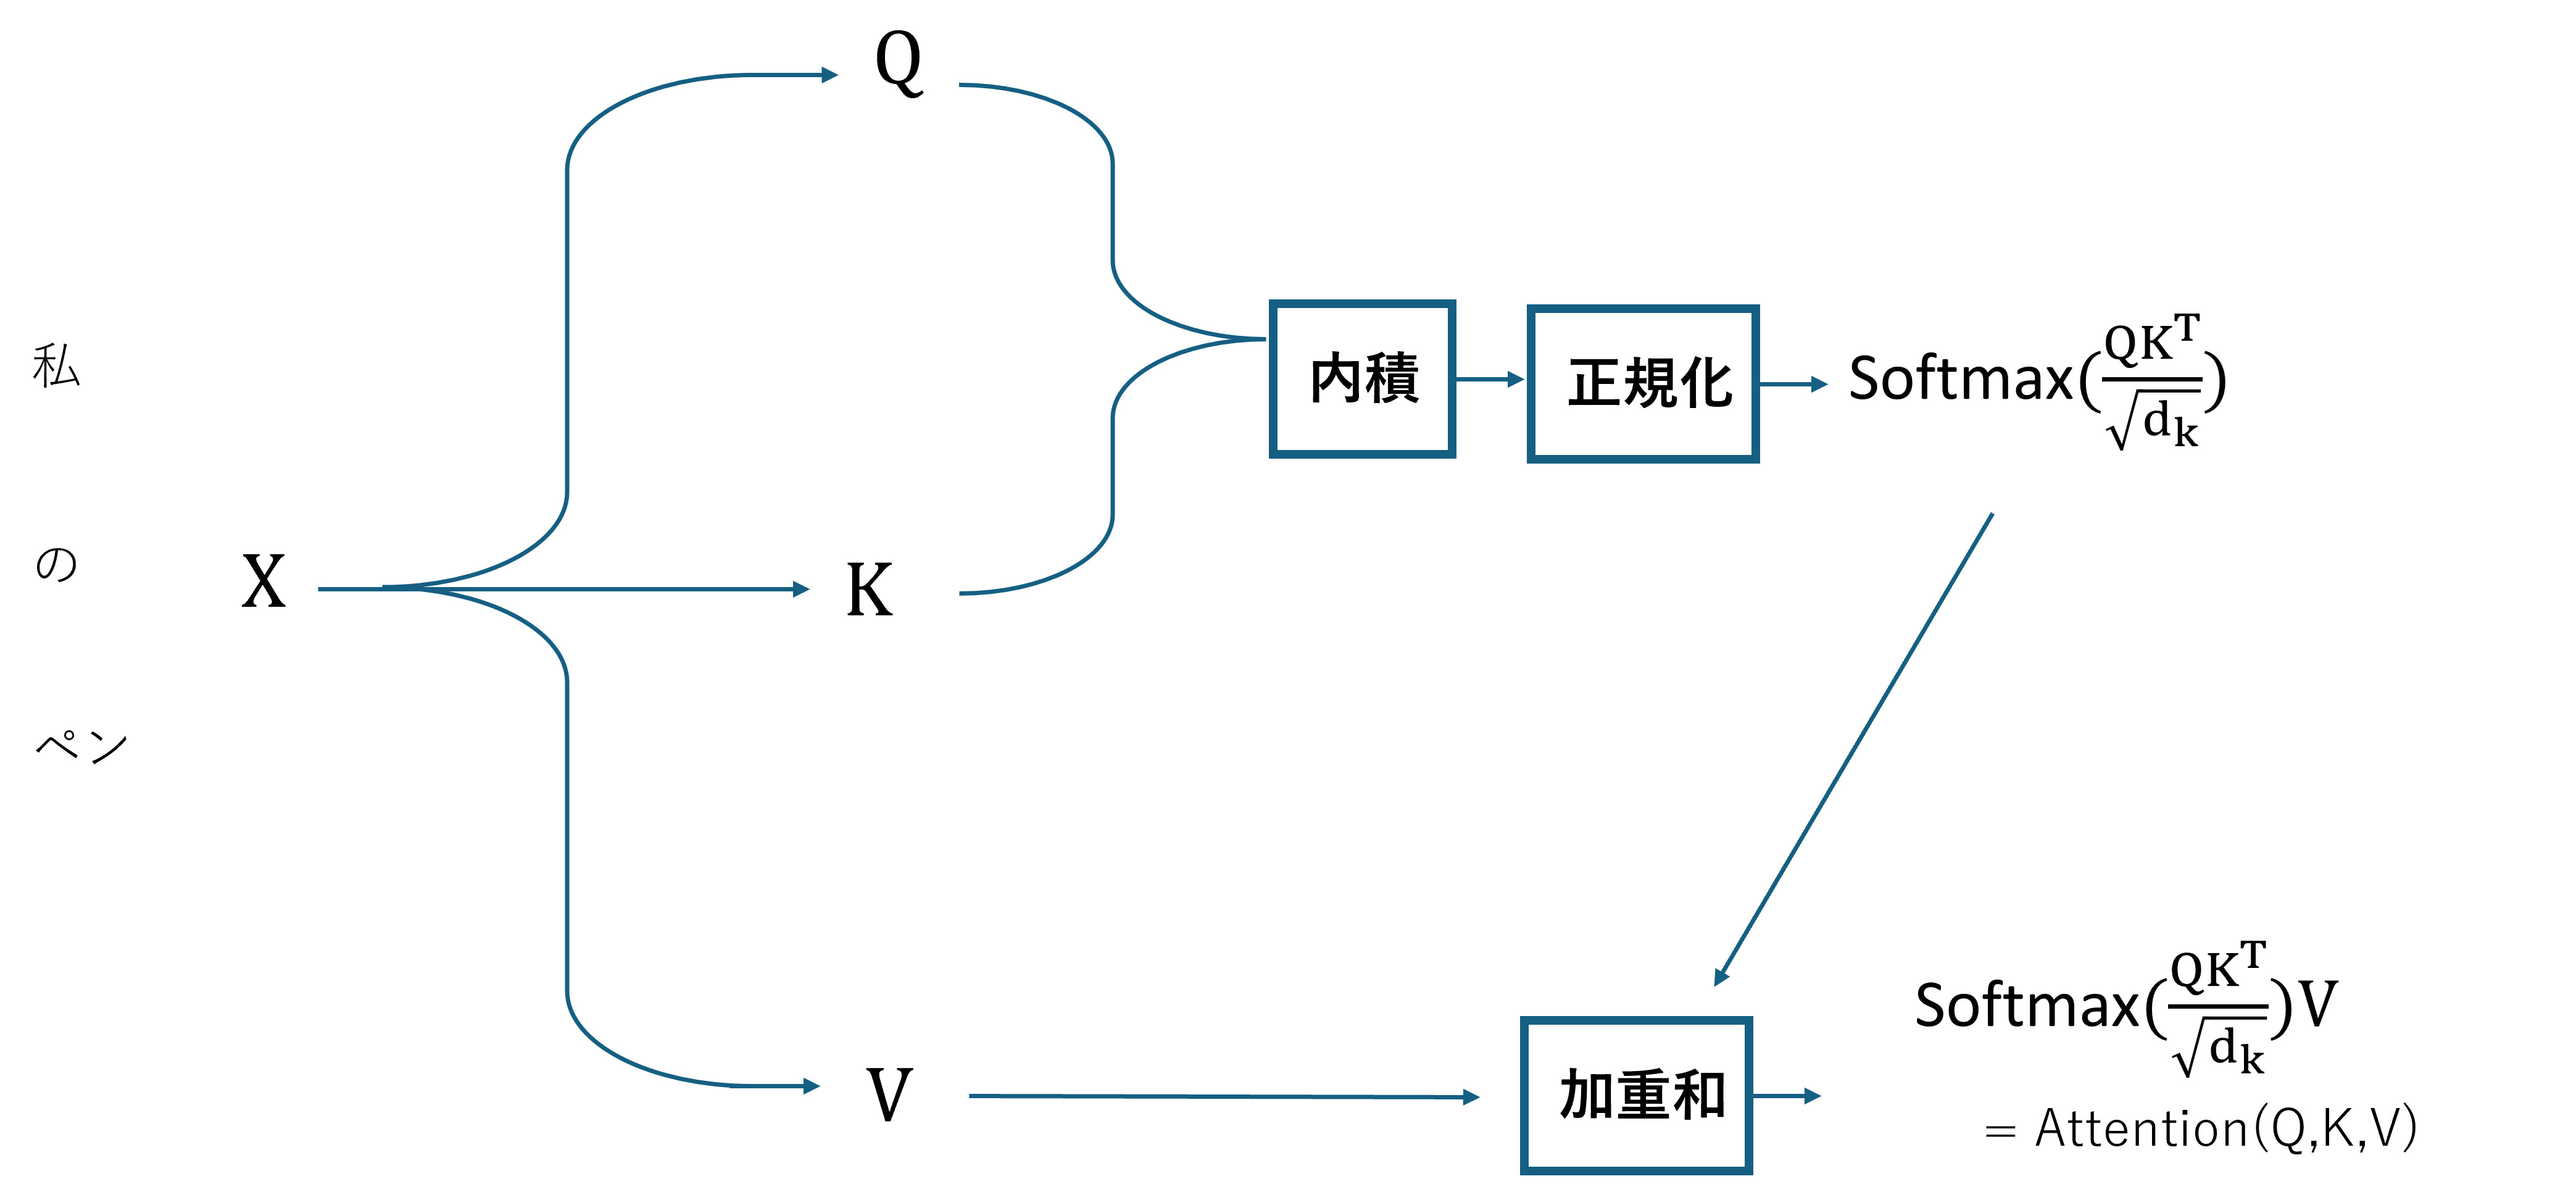
\includegraphics[width=0.8\linewidth]{Scaled Dot 4.png}
    \end{figure}
    \footnotesize
    $x_1$、$x_2$、$x_3$の更新は独立しているため並列化可能
    
    \rightarrow $x_1$を行列Xの1列目の要素のようにみなすとX全体の更新をAttention(Q,K,V)で行える

    \vspace{1em}
    \tiny
    \href{https://arxiv.org/abs/1706.03762}{Vaswani, A. et al., Attention Is All You Need, Proceedings of the 31st International Conference on Neural Information Processing Systems, pp.6000 - 6010, 2017.}
\end{frame}

\begin{frame}{Multi-Head Attention}
    \begin{columns}[c]
        \column{0.3\textwidth}
        \begin{figure}[bthp]
        \centering
        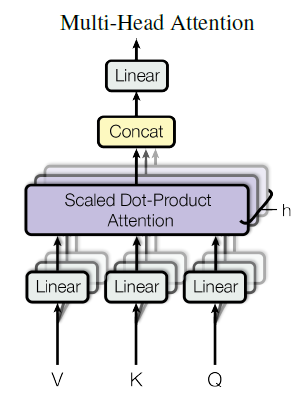
\includegraphics[width=1\linewidth]{Multi Head Attention.png}
        \end{figure}
        \column{0.7\textwidth}
        \begin{figure}[bthp]
        \centering
        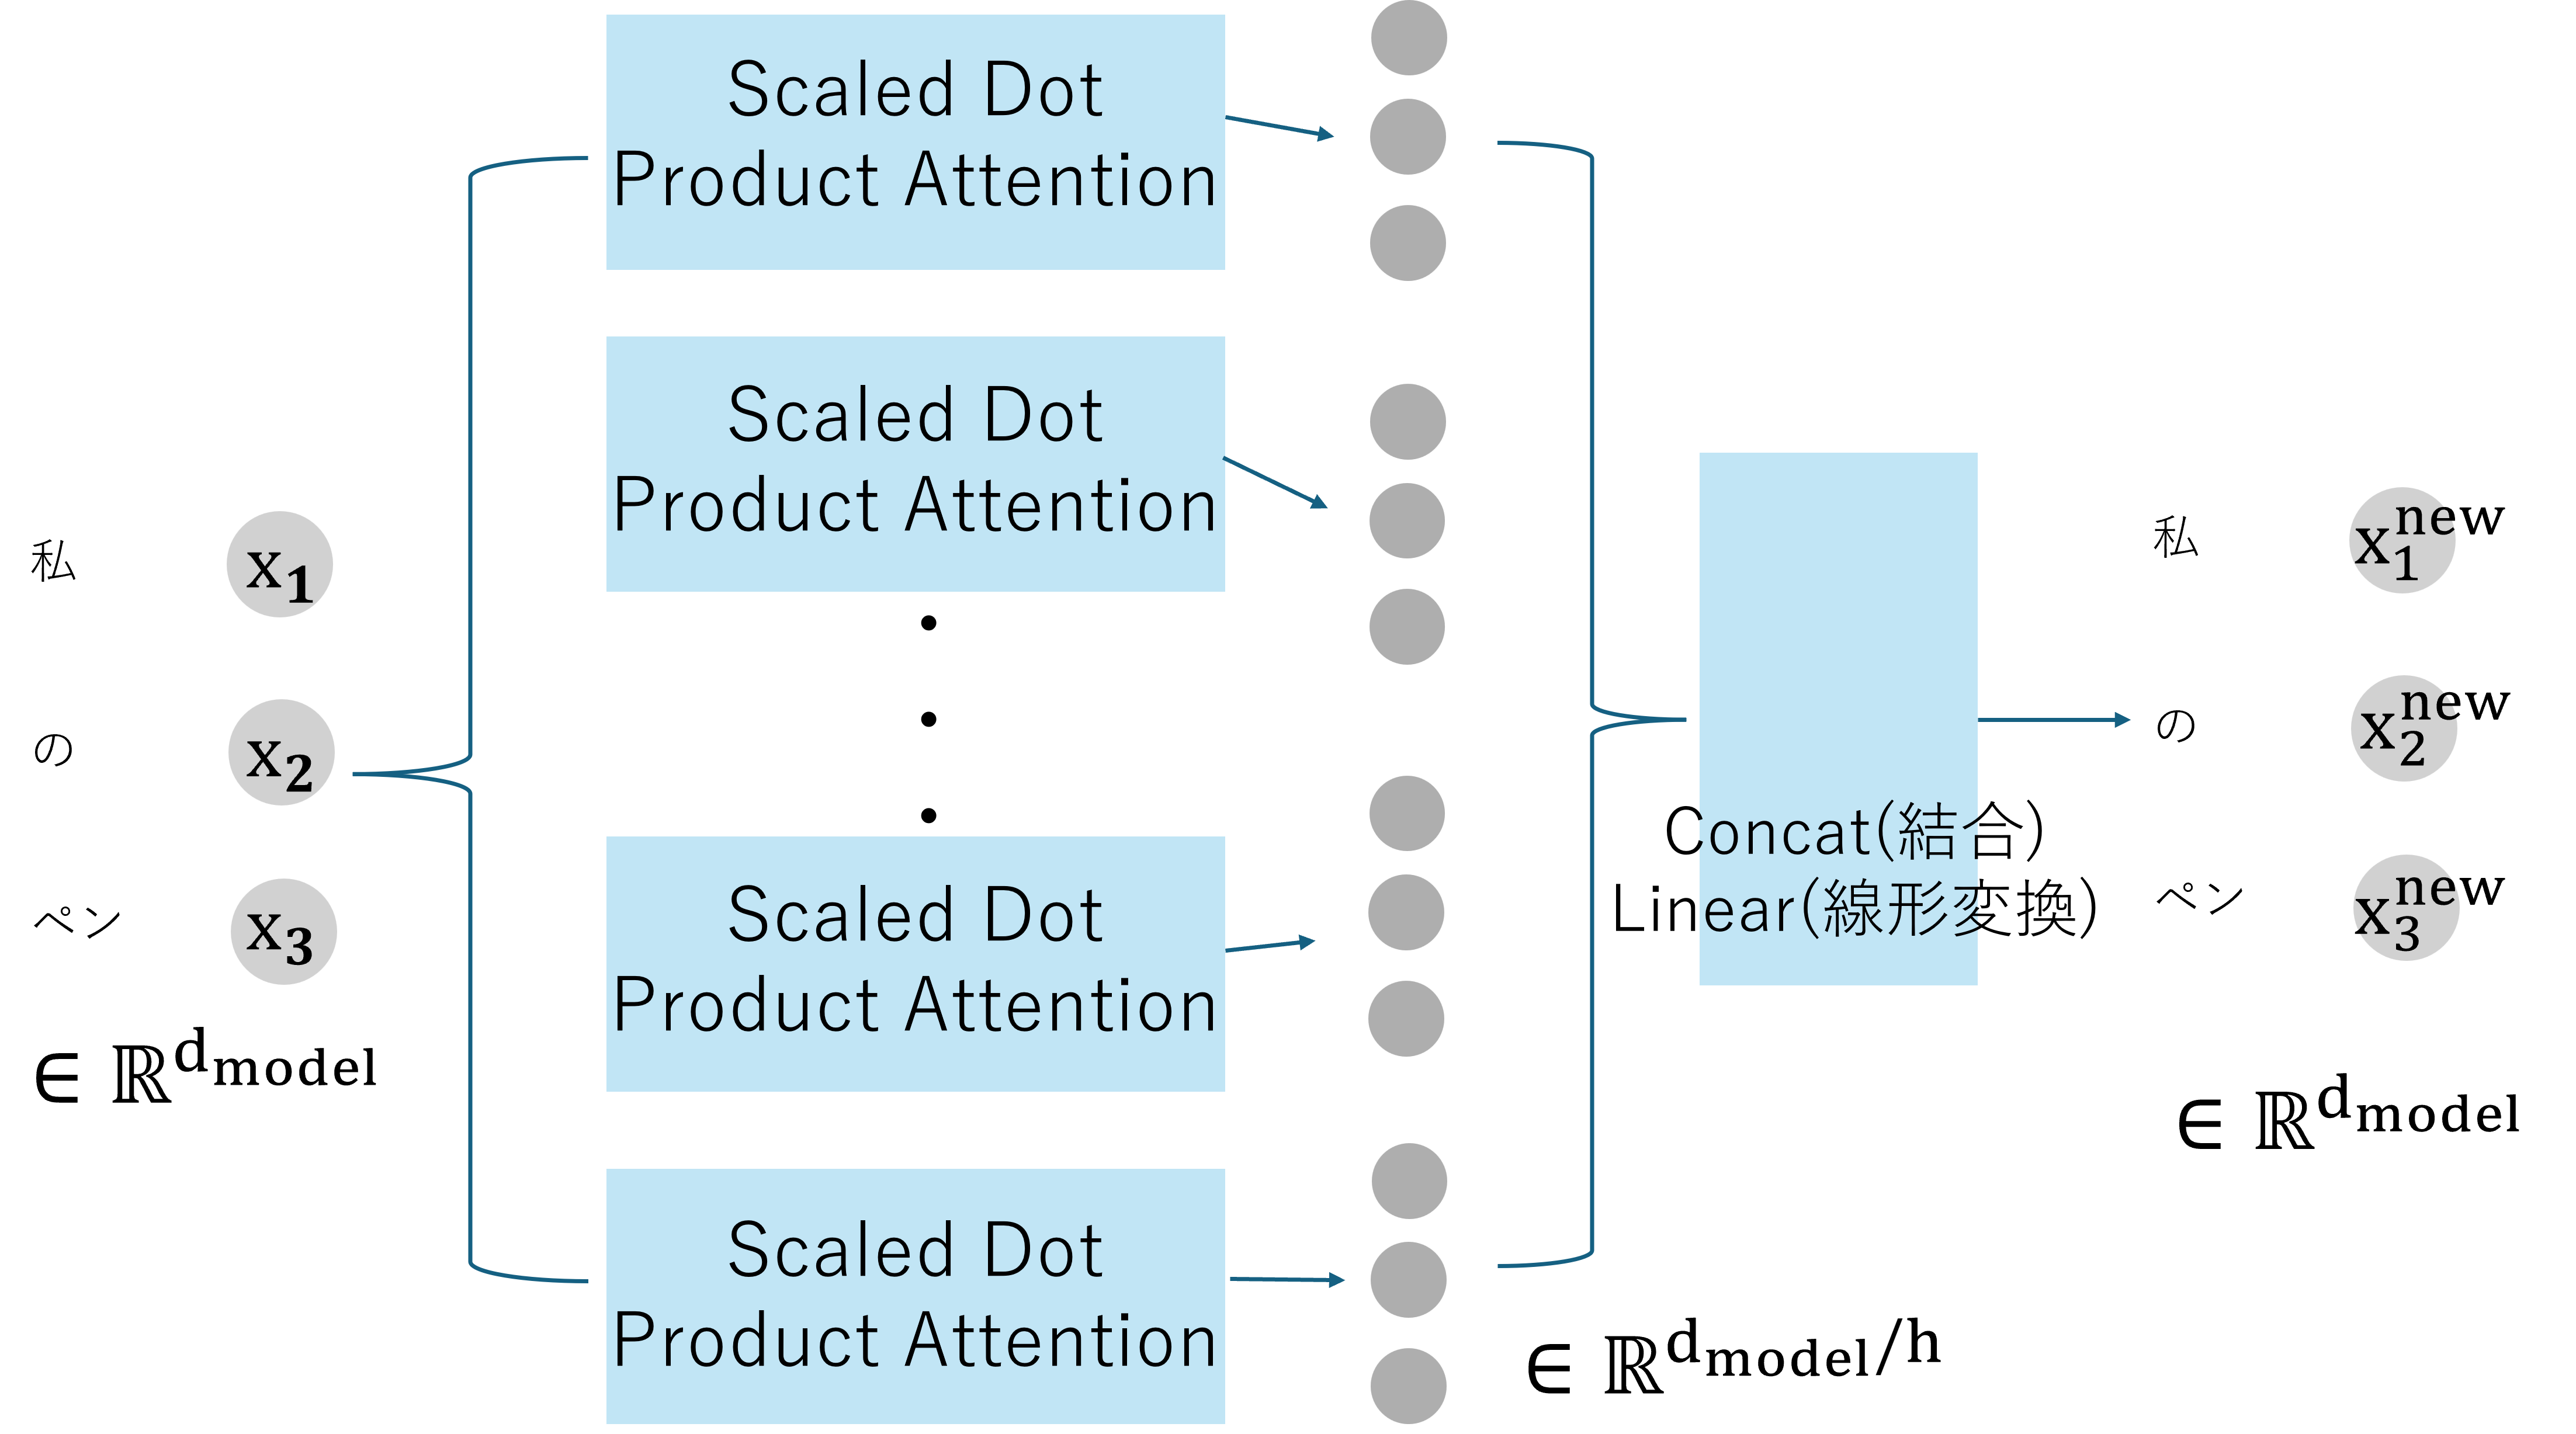
\includegraphics[width=0.9\linewidth]{Multi Head 1.png}
        \end{figure}
        \centering
        \scriptsize
        $\text{Multi Head}(Q,K,V)=\text{Concat}(\text{head}_{1},,,\text{head}_{h})W^{o}$
        $\text{head}_{i}=\text{Attentio}(QW^{Q}_{i},KW^{K}_{i},VW^{V}_{i})$
        
        \vspace{0.5em}
        \tiny
        %\small
        \begin{tabular}{lll}
            \hline
            \textbf{変数} & \textbf{名称} \\ \hline
            $W^{Q}, W^{K}\in \mathbb{R}^{d_{model} \times d_{k}}$ & Q, Kの投影用の重み  \\
            $W^{V}\in \mathbb{R}^{d_{model} \times d_{v}}$ & Vの投影用の重み \\
            $W^{O}\in \mathbb{R}^{hd_v \times d_{model}}$ & 出力統合用の重み \\
            $d_{k}, d_{v}$ & 各ヘッドの次元数 \\
            $d_{model}$ & 埋め込みベクトルの次元数 \\
            $h $ & ヘッド数 \\ \hline

        \end{tabular}
    \end{columns}
    \vspace{0.1em}
    \tiny
    \href{https://arxiv.org/abs/1706.03762}{Vaswani, A. et al., Attention Is All You Need, Proceedings of the 31st International Conference on Neural Information Processing Systems, pp.6000 - 6010, 2017.}
\end{frame}

\begin{frame}{Multi-Head Attention}
    \begin{figure}[bthp]
        \centering
        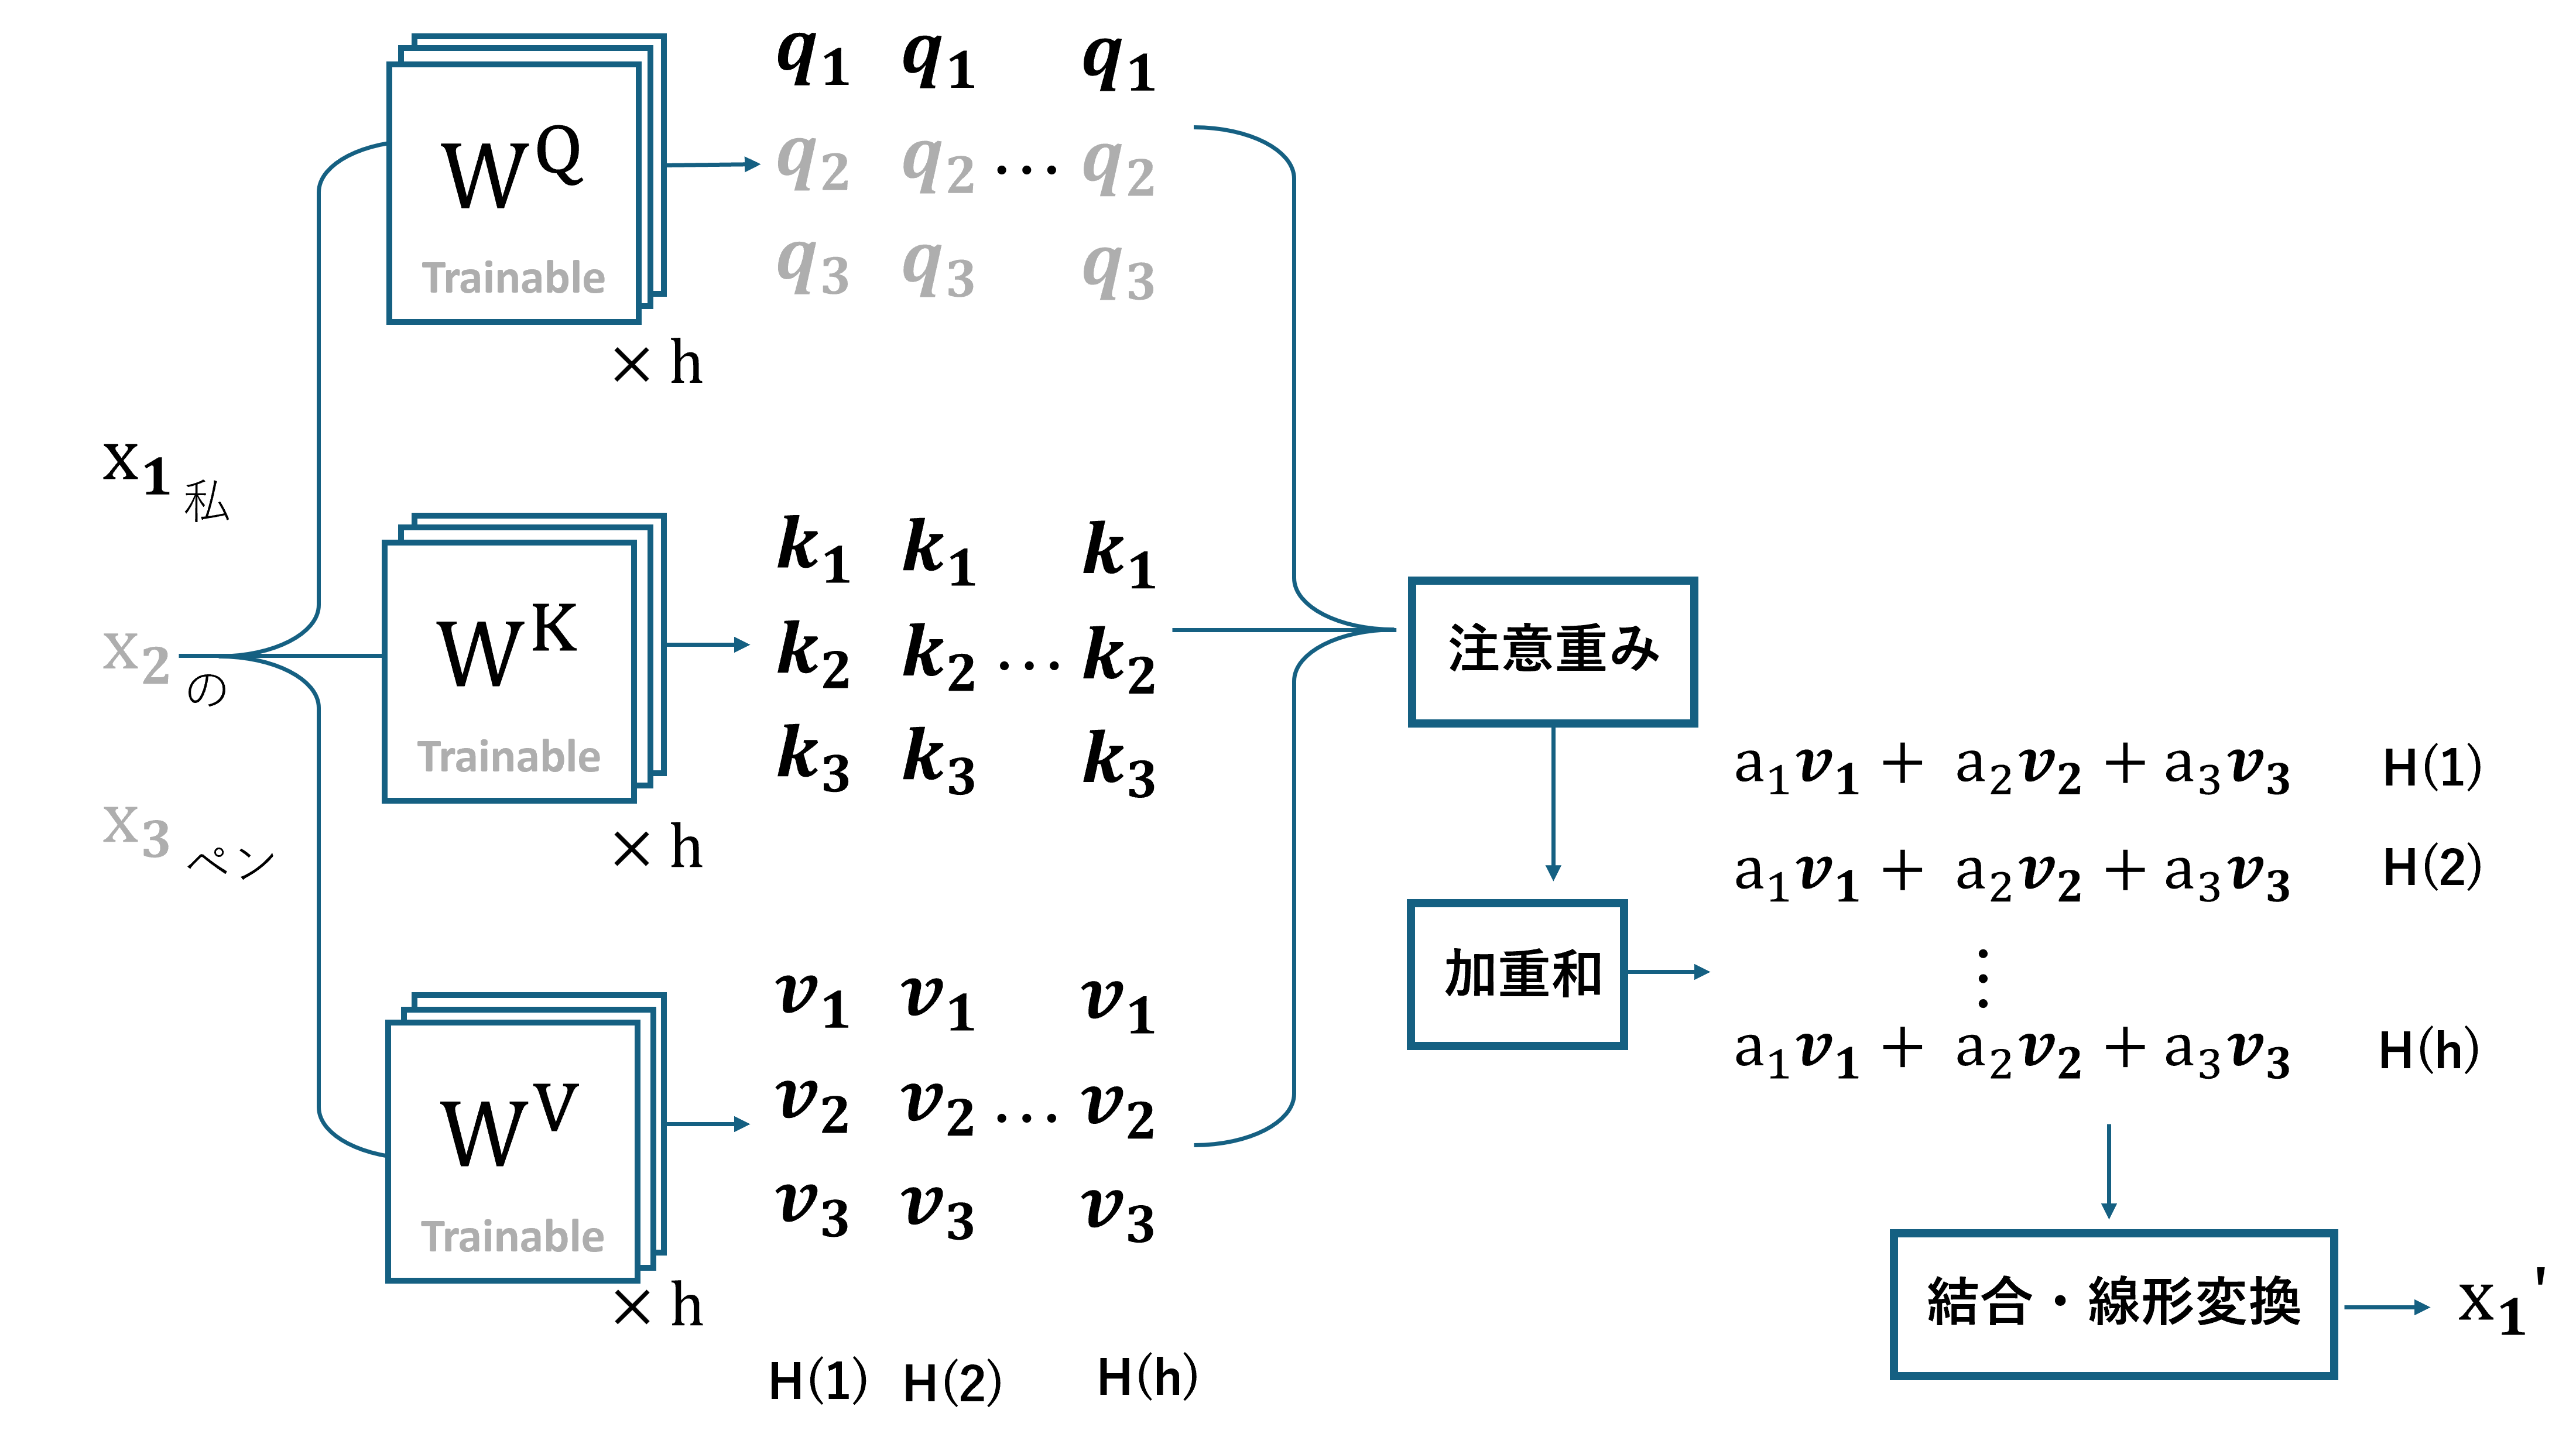
\includegraphics[width=0.8\linewidth]{Multihead Attentionイメージ.png}
    \end{figure}

    \vspace{1em}
    \tiny
    \href{https://arxiv.org/abs/1706.03762}{Vaswani, A. et al., Attention Is All You Need, Proceedings of the 31st International Conference on Neural Information Processing Systems, pp.6000 - 6010, 2017.}
\end{frame}

\begin{frame}{Masked Multi-Head Attention}
    \begin{columns}[c]
        \column{0.4\textwidth}
        \begin{figure}[bthp]
            \centering
            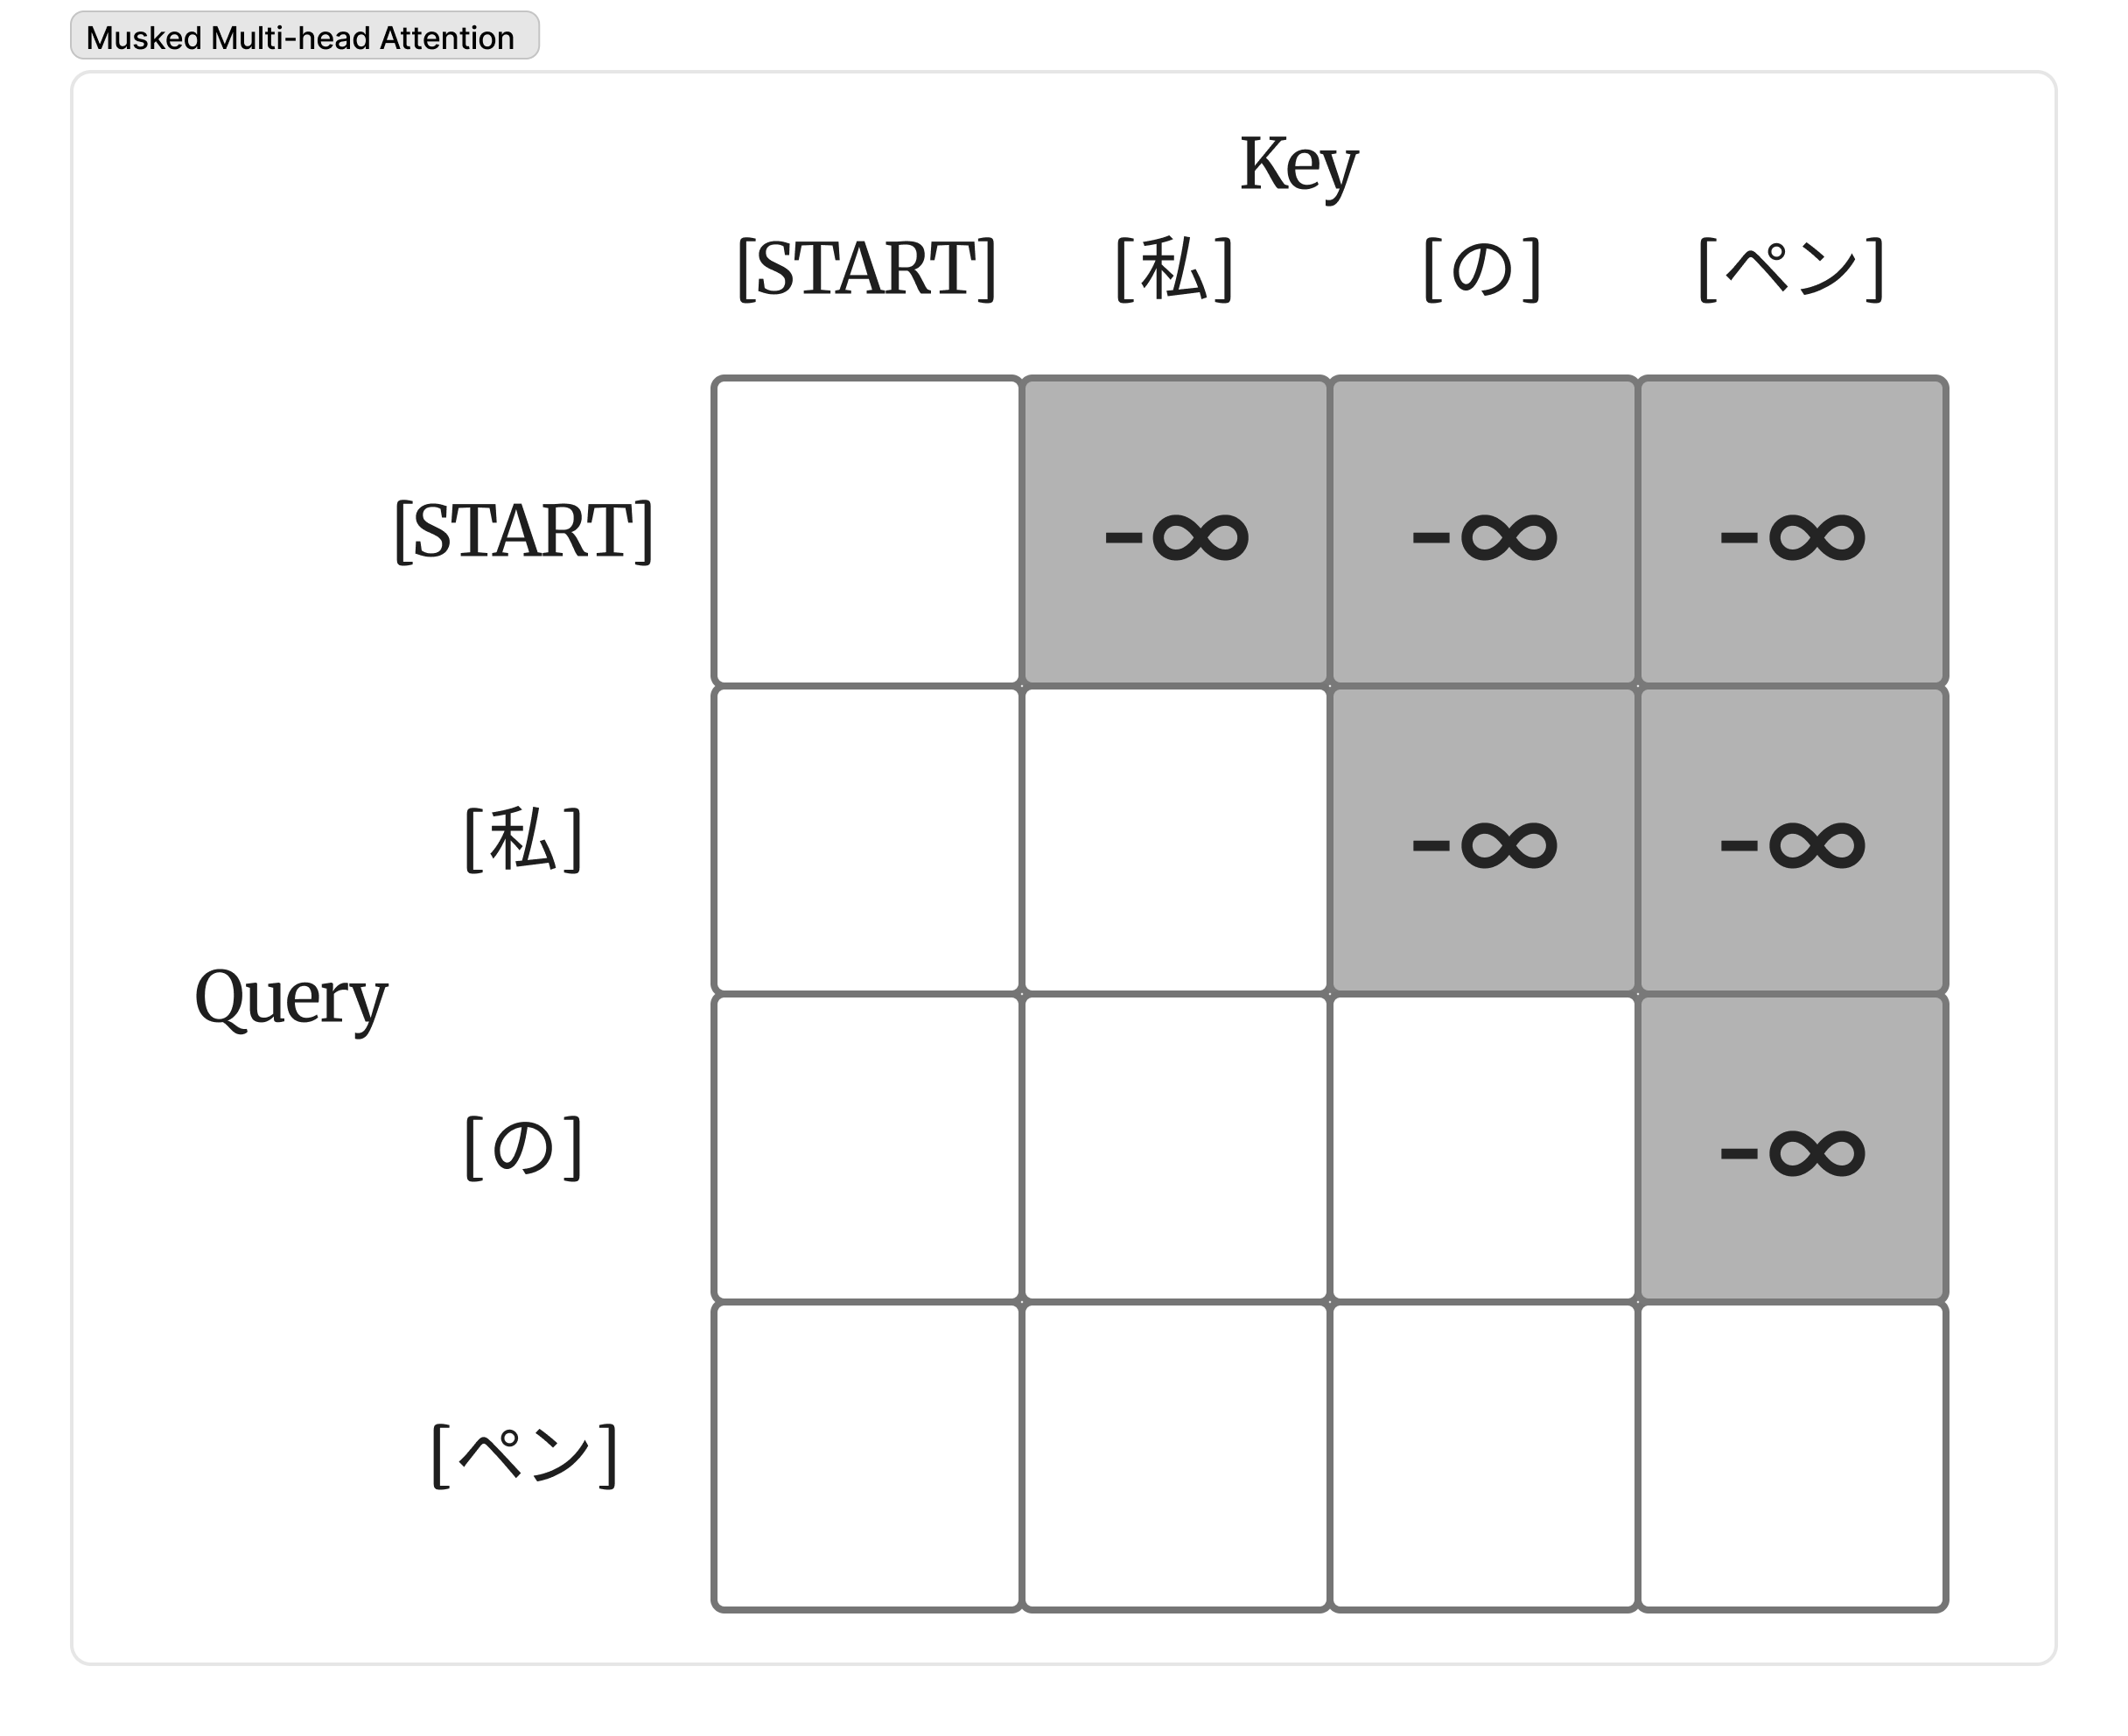
\includegraphics[width=1\linewidth]{Masked Multi-head attention.png}
        \end{figure}
        \tiny
        \begin{equation*}
            e_{ij} = 
            \begin{cases} 
                \displaystyle \frac{q_i^\top k_j}{\sqrt{d_k}} & (j \le i) \\[10pt]
                -\infty & (j > i) 
            \end{cases}
        \end{equation*}
        \column{0.55\textwidth}
        \scriptsize
        グレーのマスは自身(Query側のトークン)から見ると, 未来のトークンなので, Maskをかけてアテンションを張れないようにする. 
        Softmax直前に, 該当要素へ大きな負(-1.0e+10)の値を足す.

        \vspace{0.5em}
        \tiny
        クエリ $q_i$ に対する Attention
        \begin{equation*}
            \text{Attention}(q_i, K, V) = \sum_{j=1}^{n} \underbrace{\left( \frac{\exp\left(\frac{q_i k_j^\top}{\sqrt{d_k}}\right)}{\sum_{l=1}^{n} \exp\left(\frac{q_i k_l^\top}{\sqrt{d_k}}\right)} \right)}_{\text{Softmax による重み}} v_j
        \end{equation*}
        \tiny
        \begin{tabular}{lll}
                \hline
                \textbf{変数} & \textbf{名称} & \textbf{イメージ・定義} \\ \hline
                $Q\in \mathbb{R}^{n \times d_{k}}$ & Query &  「何に注目したいか」 \\
                $K\in \mathbb{R}^{n \times d_{k}}$ & Key & 「どのような情報を持っているか」 \\
                $V\in \mathbb{R}^{n \times d_{v}}$ & Value & 実際に抽出される「情報」 \\
                $n$ & シーケンス長 & 入力トークン数 \\
                $d_k$ & 次元数 & $Q, K$ の次元数 \\
                $d_v$ & 次元数 & $V$ の次元数 \\
                $\text{softmax}$ & 関数 & 正規化する処理 \\ \hline
            \end{tabular}
    \end{columns}
    \vspace{0.5em}
    \tiny
    \href{https://arxiv.org/abs/1706.03762}{Vaswani, A. et al., Attention Is All You Need, Proceedings of the 31st International Conference on Neural Information Processing Systems, pp.6000 - 6010, 2017.}
\end{frame}

\begin{frame}{Cross Attention}
    \begin{columns}[c]
        \column{0.4\textwidth}
        \begin{figure}[bthp]
            \centering
            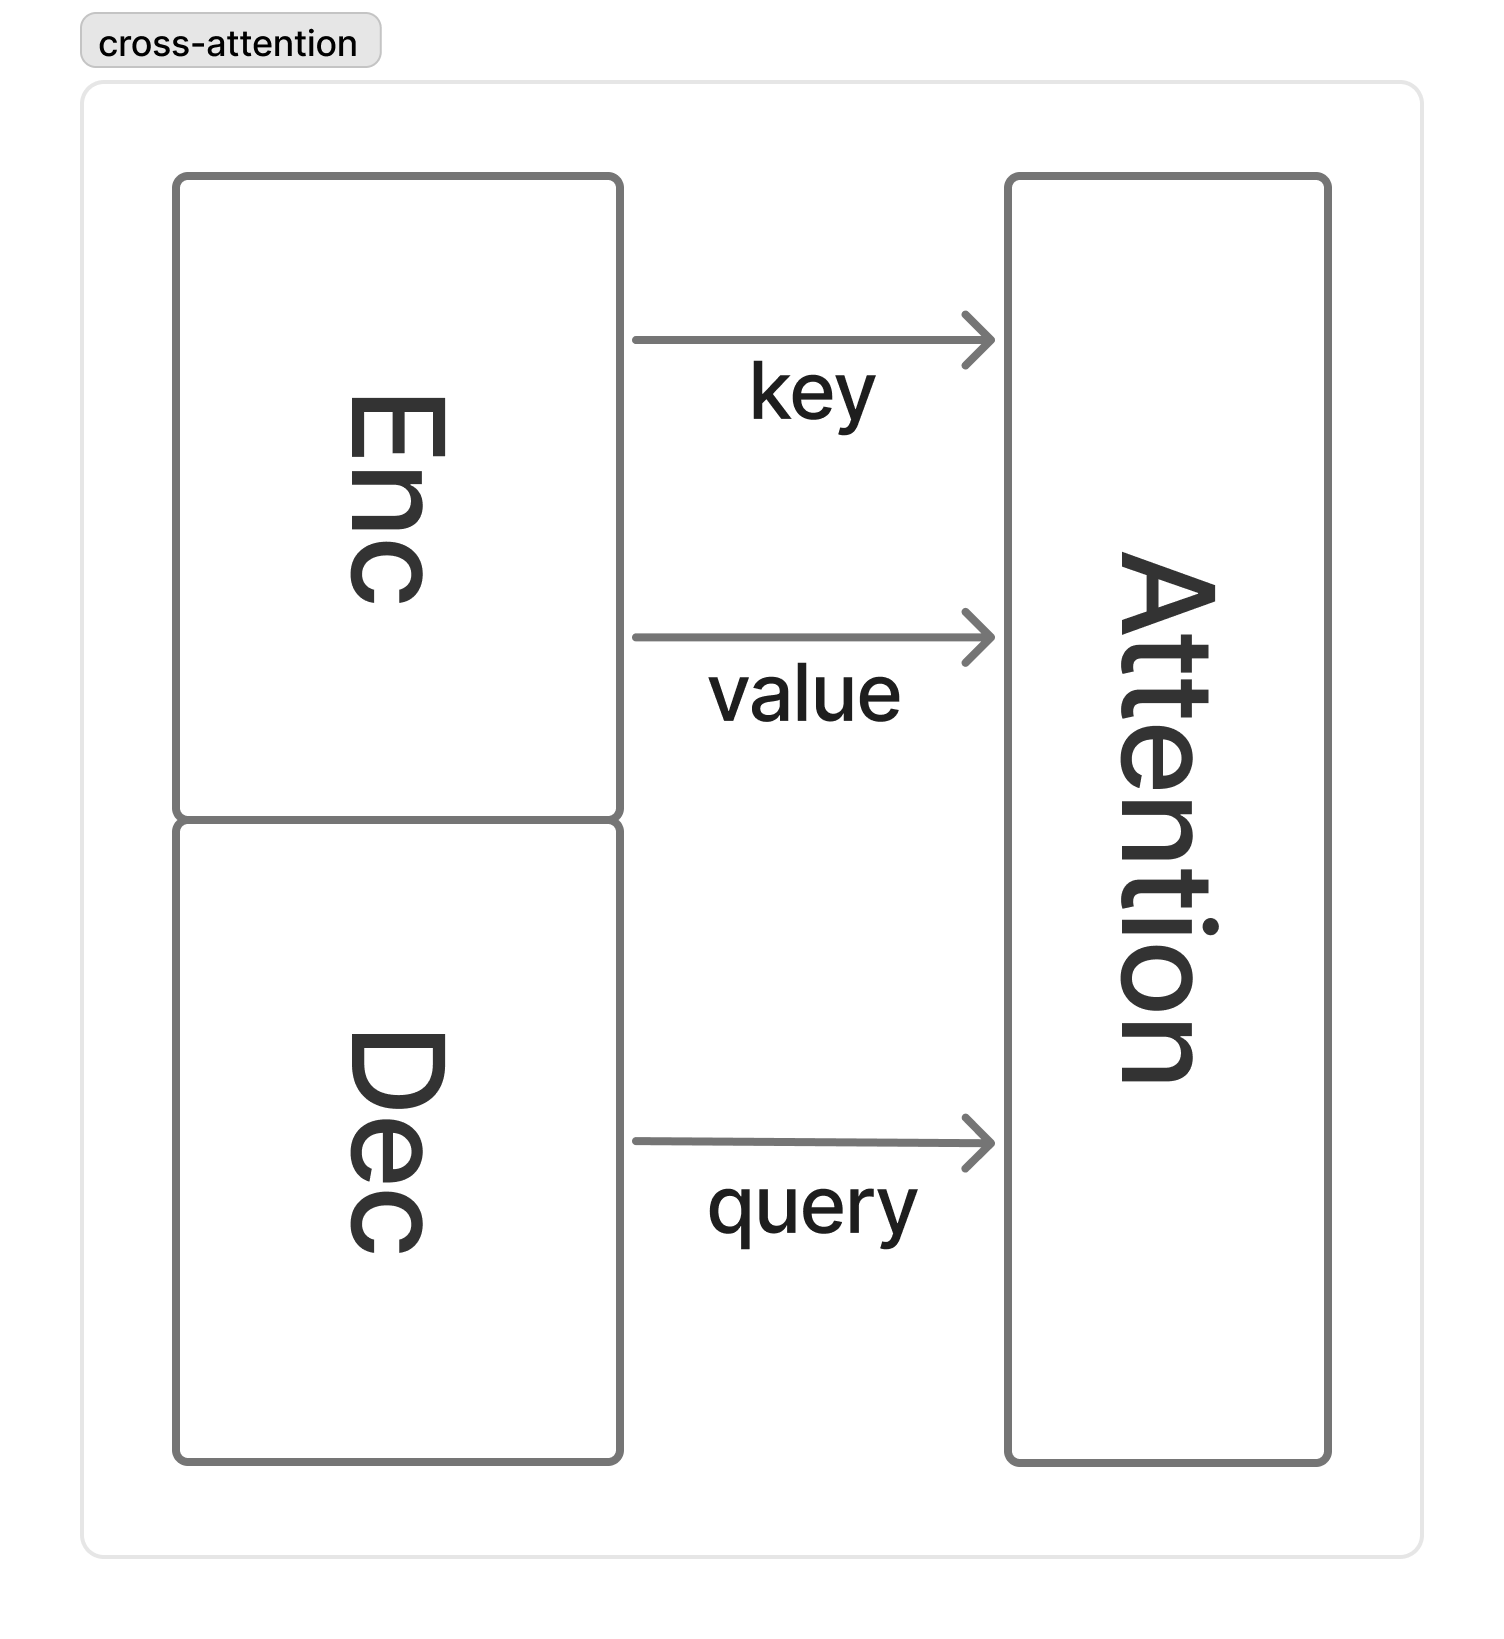
\includegraphics[width=1\linewidth]{cross attention.png}
        \end{figure}
        \column{0.55\textwidth}
        \scriptsize
        Attention計算時にkeyとvalueをencderのベクトル列から取得し, queryをdecoderのベクトル列から取得することで, 2つの系列の情報を統合する
    \end{columns}
    \vspace{0.5em}
    \tiny
    \href{https://arxiv.org/abs/1706.03762}{Vaswani, A. et al., Attention Is All You Need, Proceedings of the 31st International Conference on Neural Information Processing Systems, pp.6000 - 6010, 2017.}
\end{frame}

\begin{frame}{モデル構造 - Feed Forward}
    \framesubtitle{Transformer}
    \vspace{-0.5em}
    \begin{columns}[c]
        \column{0.5\textwidth}
        \begin{figure}[bthp]
        \centering
        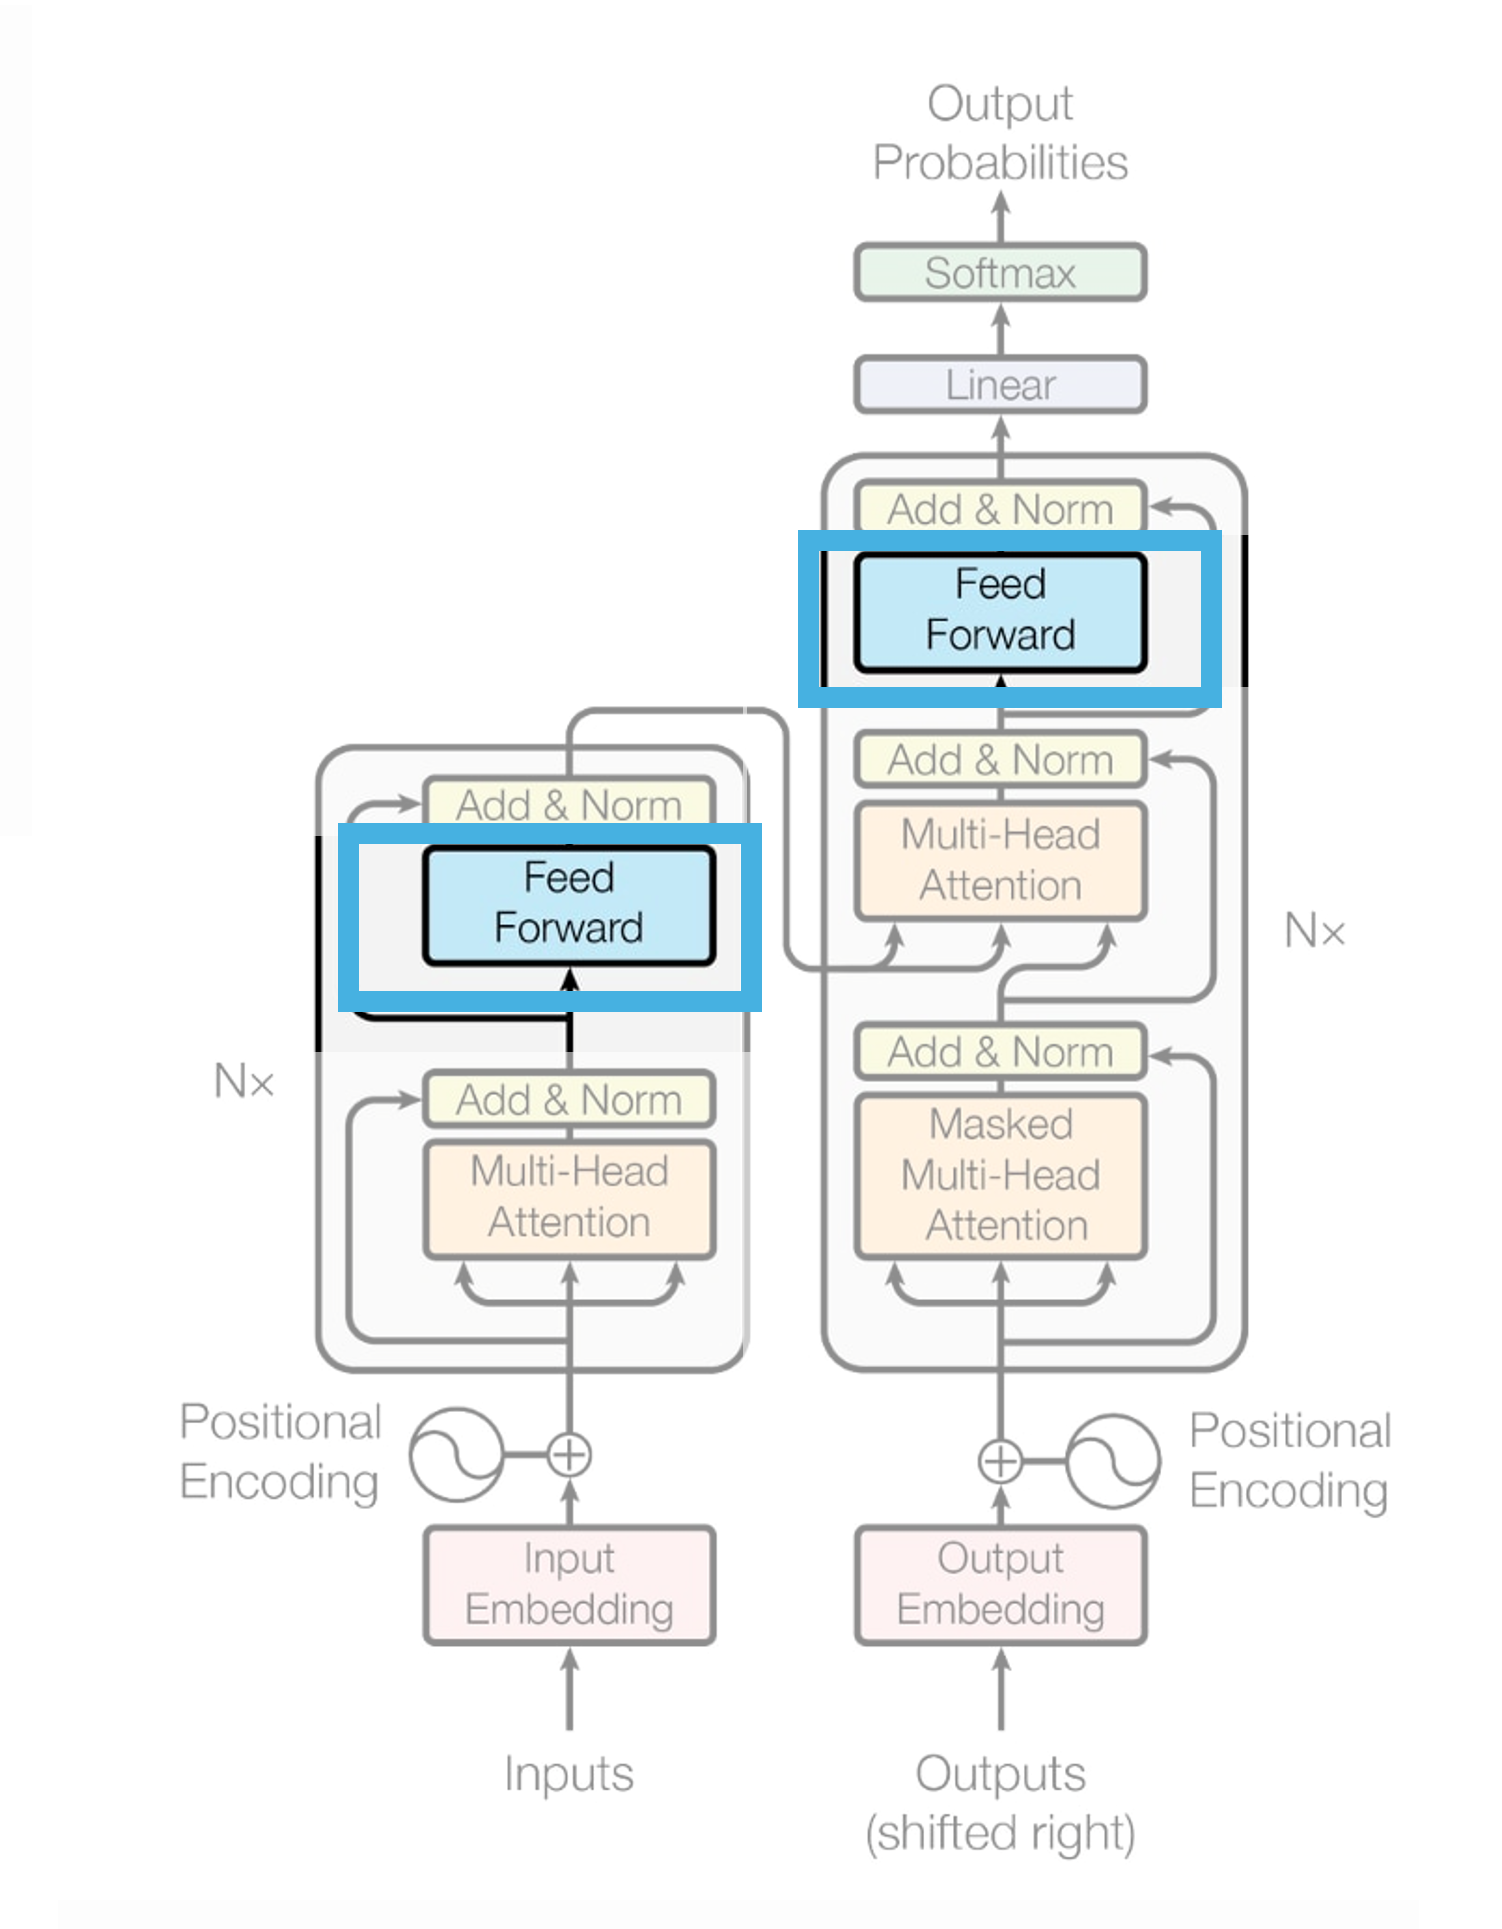
\includegraphics[width=1\linewidth]{Transformer_feedforward.png}
        \end{figure}
        \column{0.45\textwidth}
        \small
        \begin{itemize}
            \item Embedding
            \item Multi-Head Attention
            \item \textcolor{cyan}{FeedForward}
            \item Others
        \end{itemize}
        \vspace{0.7em}
        \tiny
        \href{https://arxiv.org/abs/1706.03762}{Vaswani, A. et al., Attention Is All You Need, Proceedings of the 31st International Conference on Neural Information Processing Systems, pp.6000 - 6010, 2017.}
    \end{columns}
\end{frame}

\begin{frame}{Feed Forward Network(FFN)}
    \begin{columns}[c]
        \column{0.45\textwidth}
        \begin{figure}[bthp]
        \centering
        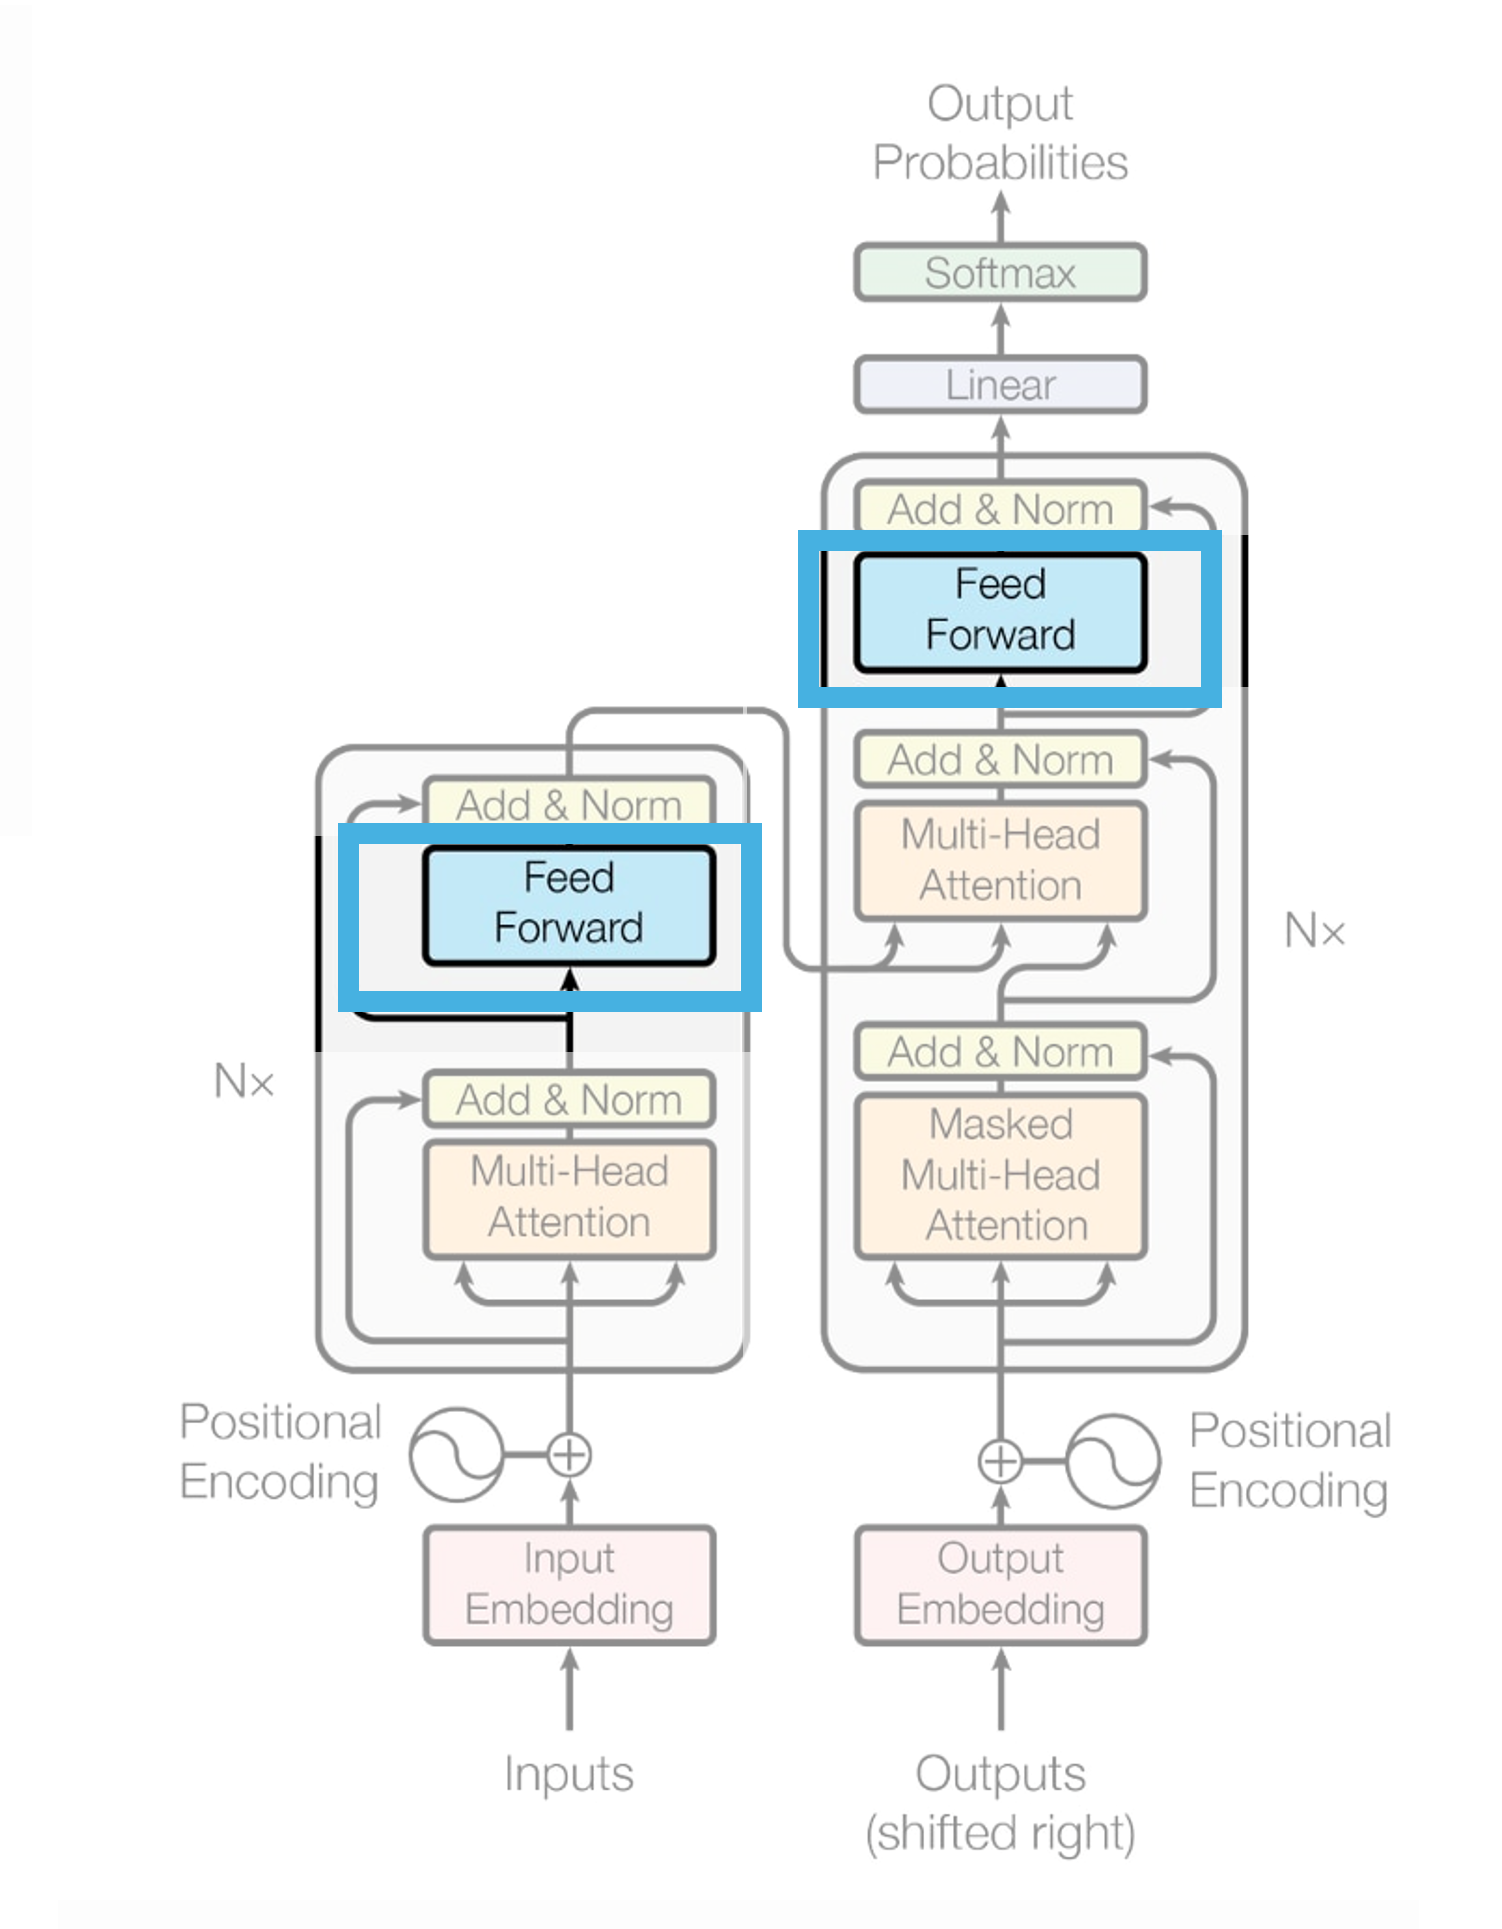
\includegraphics[width=1\linewidth]{Transformer_feedforward.png}
        \end{figure}

        \column{0.5\textwidth}
        \begin{figure}[bthp]
        \centering
        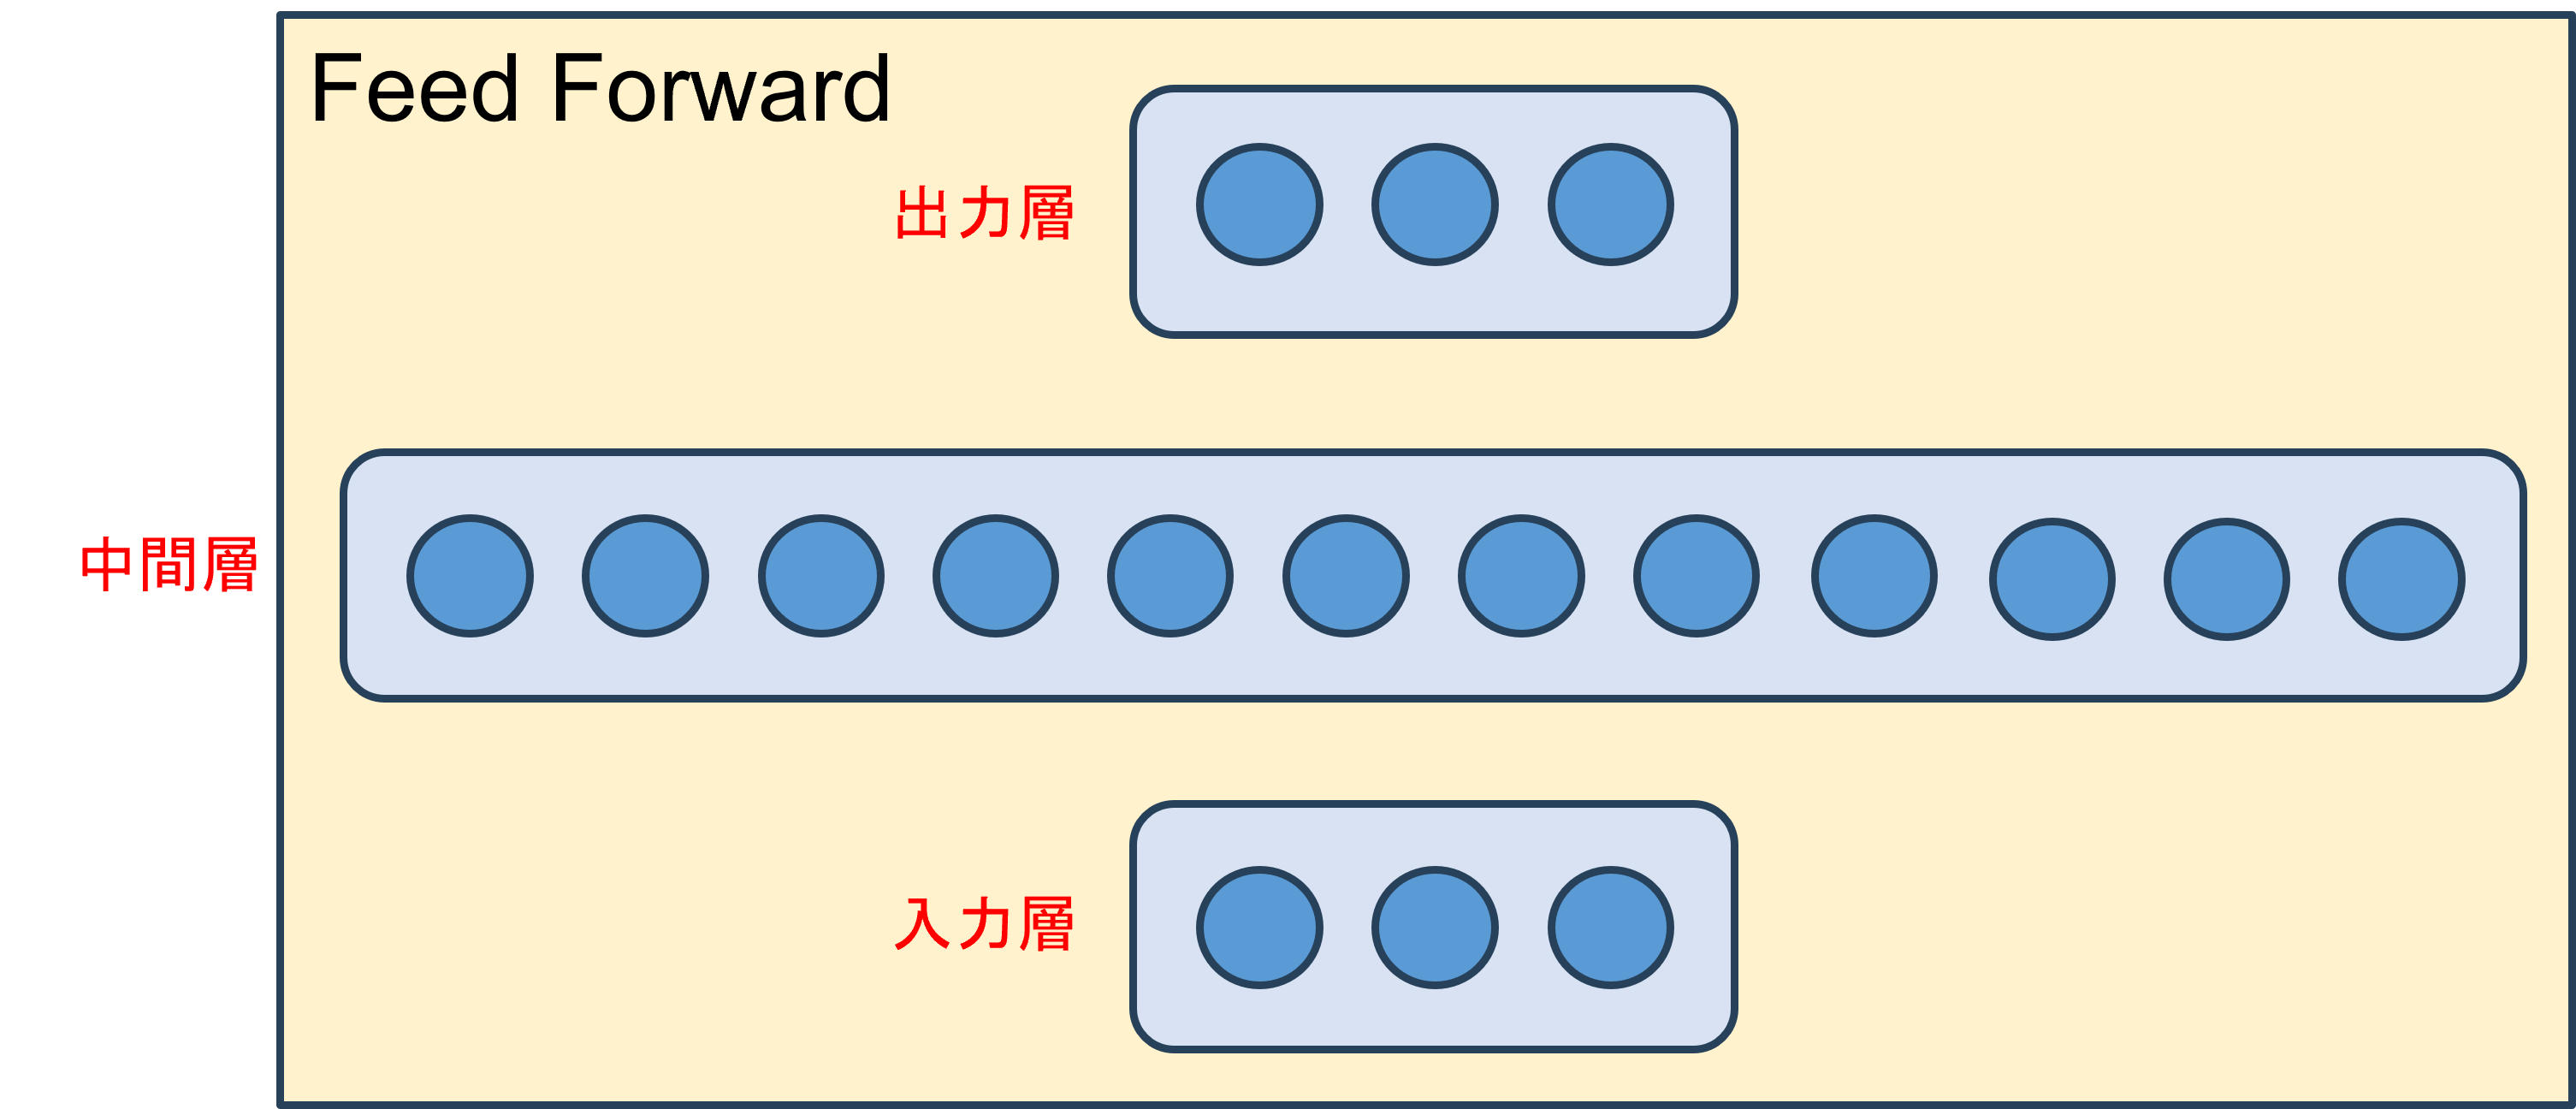
\includegraphics[width=1\linewidth]{FFN_image.png}
        \end{figure}
        \footnotesize
        \begin{align*}
                \text{FFN}(x) = \max(0, xW_1 + b_1)W_2 + b_2
        \end{align*}
        \tiny
        %\small
        \begin{tabular}{ll}
            \hline
            \textbf{変数} & \textbf{名称} \\ \hline
            $W_{1}\in \mathbb{R}^{d_{model} \times d_{ff}}$ & 学習パラメータ  \\
            $W_{2}\in \mathbb{R}^{d_{ff} \times d_{model}}$ & 学習パラメータ \\
            $b_{1}\in \mathbb{R}^{d \times d}$ & 学習パラメータ  \\
            $b_{2}\in \mathbb{R}^{d \times d}$ & 学習パラメータ \\
            $max(0, ..)$ & ReLU関数 \\
            $d_{model}$ & 埋め込みベクトルの次元数 \\
            $d_{ff}$ & FFNの中間層の次元数($d_{model}の4倍$) \\\hline
        \end{tabular}
    \end{columns}
    \vspace{0.5em}
    \tiny
    \href{https://arxiv.org/abs/1706.03762}{Vaswani, A. et al., Attention Is All You Need, Proceedings of the 31st International Conference on Neural Information Processing Systems, pp.6000 - 6010, 2017.}
\end{frame}

\begin{frame}{モデル構造 - Others}
    \framesubtitle{Transformer}
    \vspace{-0.5em}
    \begin{columns}[c]
        \column{0.5\textwidth}
        \begin{figure}[bthp]
        \centering
        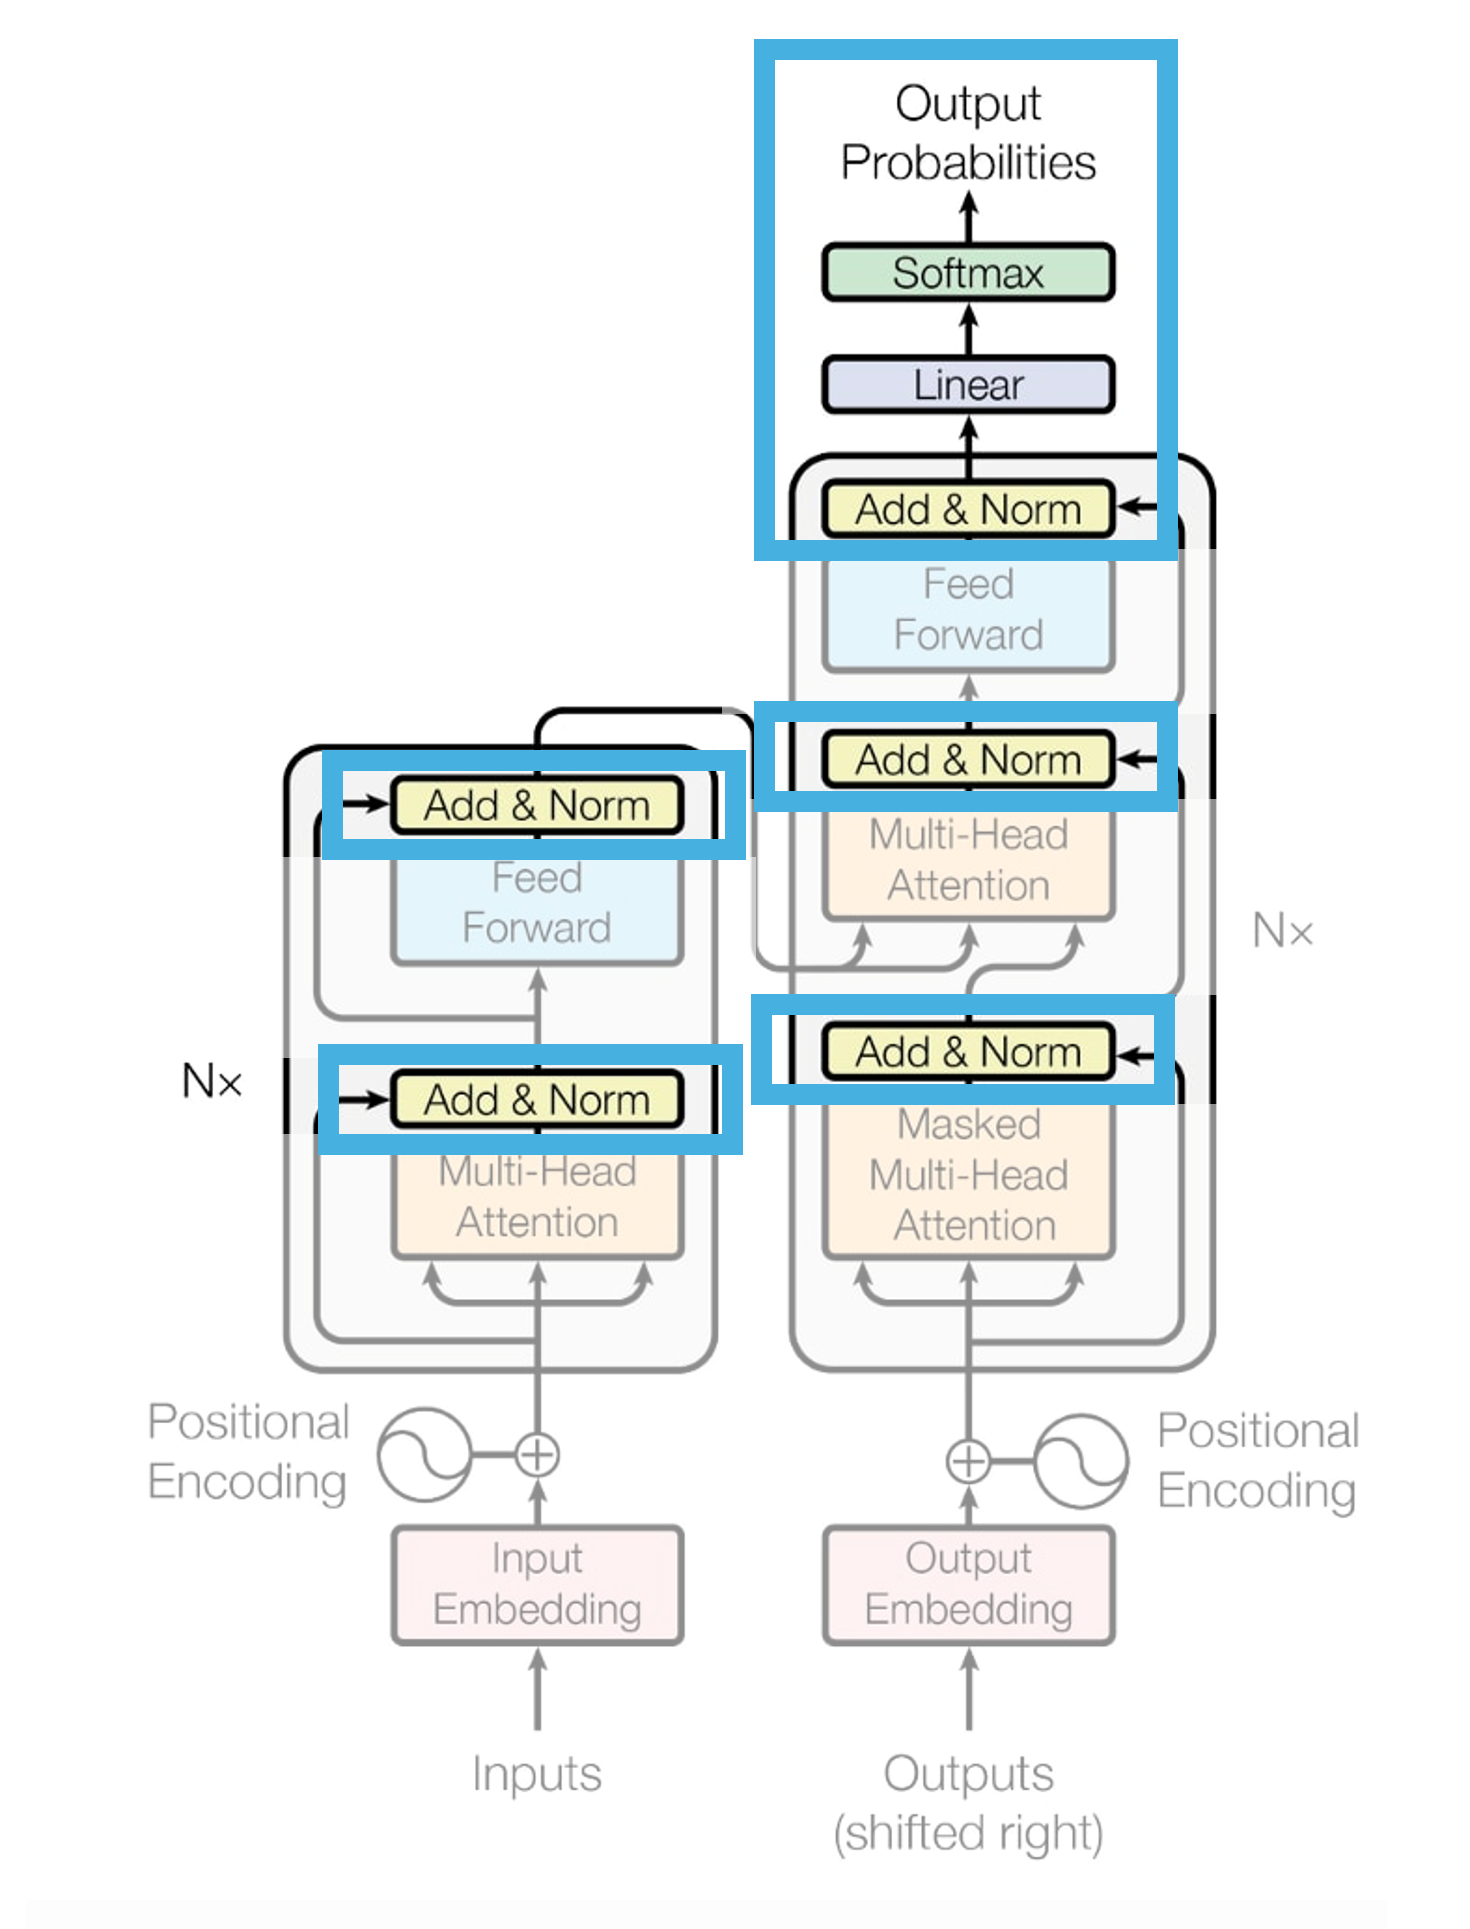
\includegraphics[width=1\linewidth]{Transformer_others.png}
        \end{figure}
        \column{0.45\textwidth}
        \small
        \begin{itemize}
            \item Embedding
            \item Multi-Head Attention
            \item Feed Forward
            \item \textcolor{cyan}{Others}
        \end{itemize}
        \vspace{0.7em}
        \tiny
        \href{https://arxiv.org/abs/1706.03762}{Vaswani, A. et al., Attention Is All You Need, Proceedings of the 31st International Conference on Neural Information Processing Systems, pp.6000 - 6010, 2017.}
    \end{columns}
\end{frame}

\begin{frame}{Add \& Norm}
    \vspace{-0.5em}
    \begin{columns}[c]
        \column{0.5\textwidth}
        \begin{figure}[bthp]
        \centering
        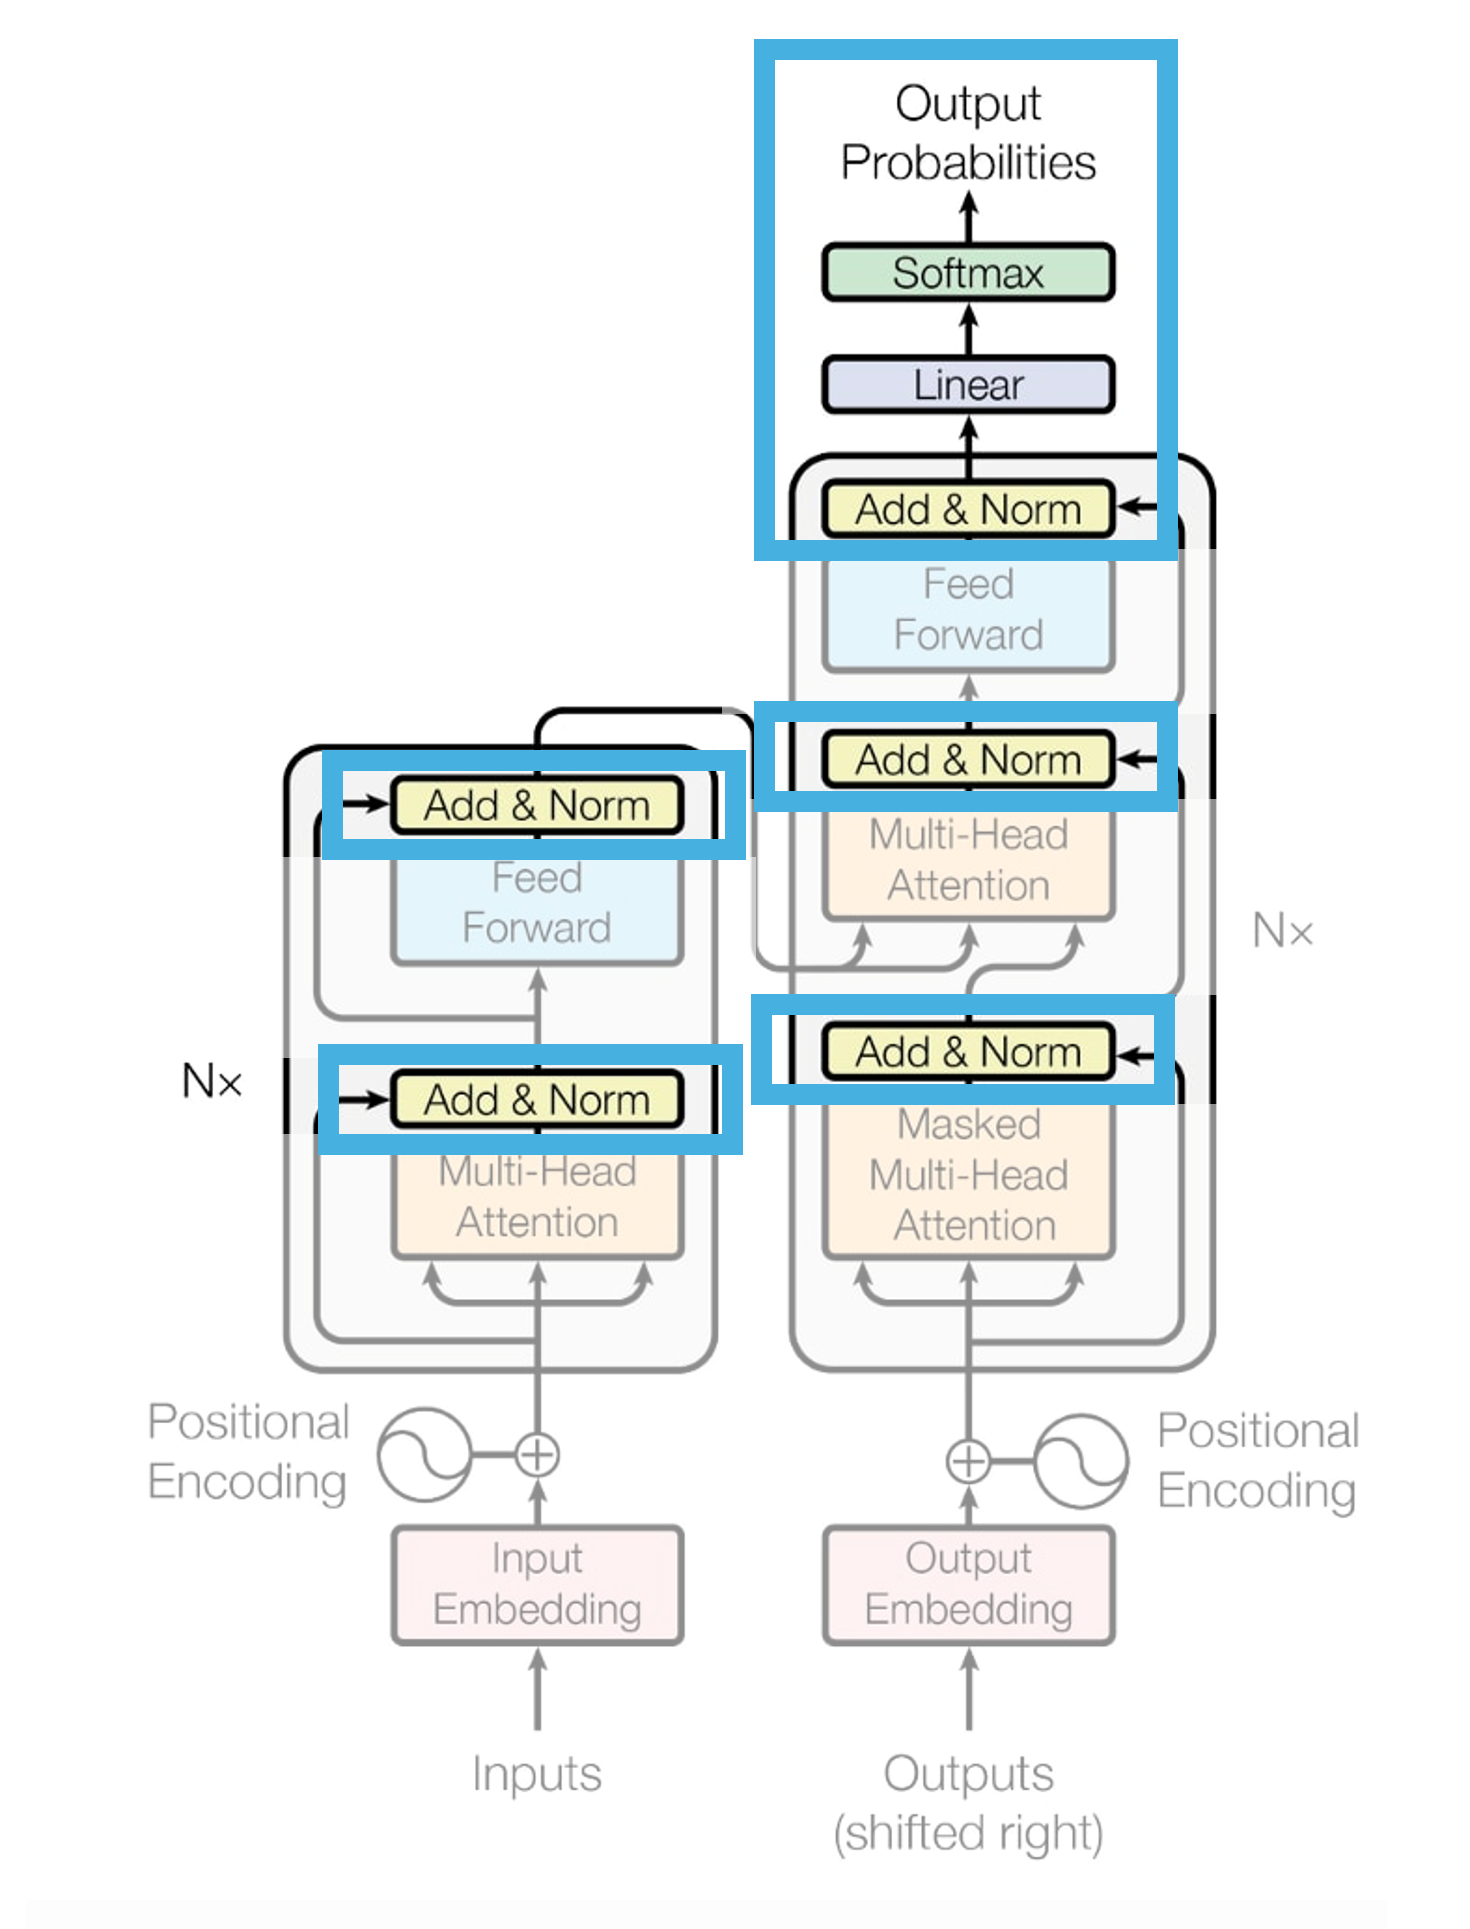
\includegraphics[width=1\linewidth]{Transformer_others.png}
        \end{figure}
        \column{0.45\textwidth}
        \scriptsize
        \begin{itemize}
            \item Add：残差接続(residual connection)
            \begin{itemize}
                \item 深い層の学習をする時のテク
                \item Feedforwardの前後で残差接続
                \item Attentionの前後で残差接続
            \end{itemize}
            \item Norm：層正規化(Layer Normalization)
            \begin{itemize}
                \item 学習を効率化するテク
                \item 隠れ層の次元軸で平均と分散をとり正規化
            \end{itemize}
        \end{itemize}
        %\vspace{0.7em}
        \tiny
        \href{https://arxiv.org/abs/1706.03762}{Vaswani, A. et al., Attention Is All You Need, Proceedings of the 31st International Conference on Neural Information Processing Systems, pp.6000 - 6010, 2017.}
    \end{columns}
\end{frame}

\begin{frame}{Add \& Norm}
    \vspace{-0.5em}
    \begin{columns}[c]
        \column{0.5\textwidth}
        \begin{figure}[bthp]
        \centering
        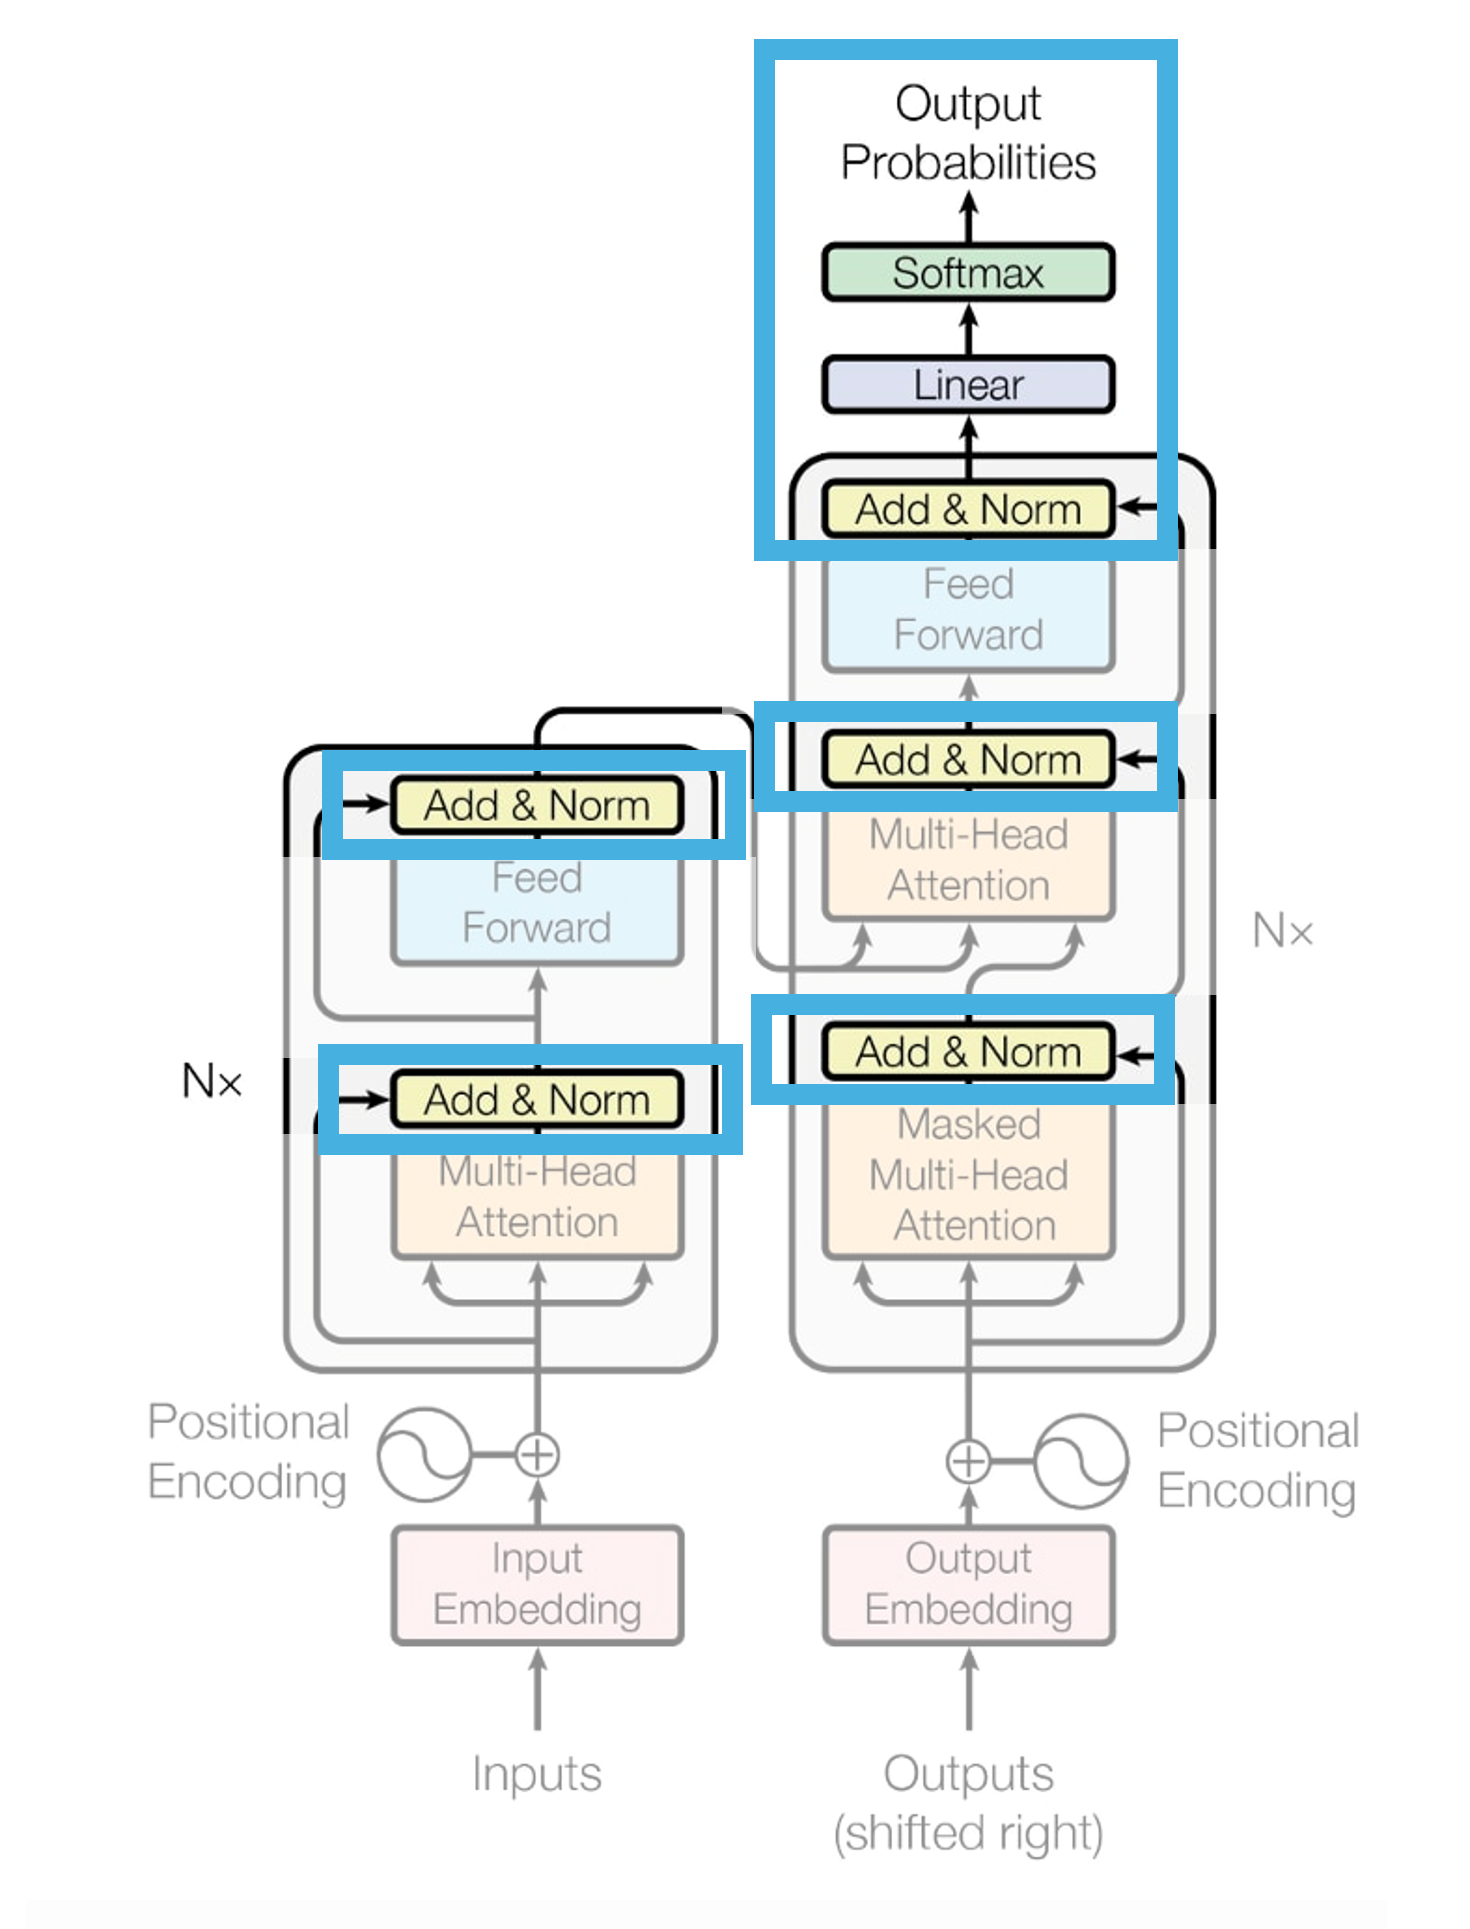
\includegraphics[width=1\linewidth]{Transformer_others.png}
        \end{figure}
        \column{0.45\textwidth}
        \scriptsize
        各サブレイヤの出力を以下の処理を行う
            \begin{align*}
                \text{Output} = \text{LayerNorm}(x + \text{Sublayer}(x))
            \end{align*}
            \begin{itemize}
                \item \textbf{Add (Residual)}: 前の層の出力$\text{Sublayer}(x)$へ入力 $x$ を直接足す
                
                \rightarrow 勾配消失を防ぎ、深い層でも学習が安定
                \item \textbf{LayerNorm}: 特徴ベクトルの平均を0、分散を1に正規化
                
                \rightarrow 学習が高速化・安定化
            \end{itemize}
        \vspace{0.7em}
        \tiny
        \href{https://arxiv.org/abs/1706.03762}{Vaswani, A. et al., Attention Is All You Need, Proceedings of the 31st International Conference on Neural Information Processing Systems, pp.6000 - 6010, 2017.}
    \end{columns}
\end{frame}

\section{Attentionの応用}
\begin{frame}{Multi-head Attentionの派生}
    \begin{figure}[bthp]
    \centering
    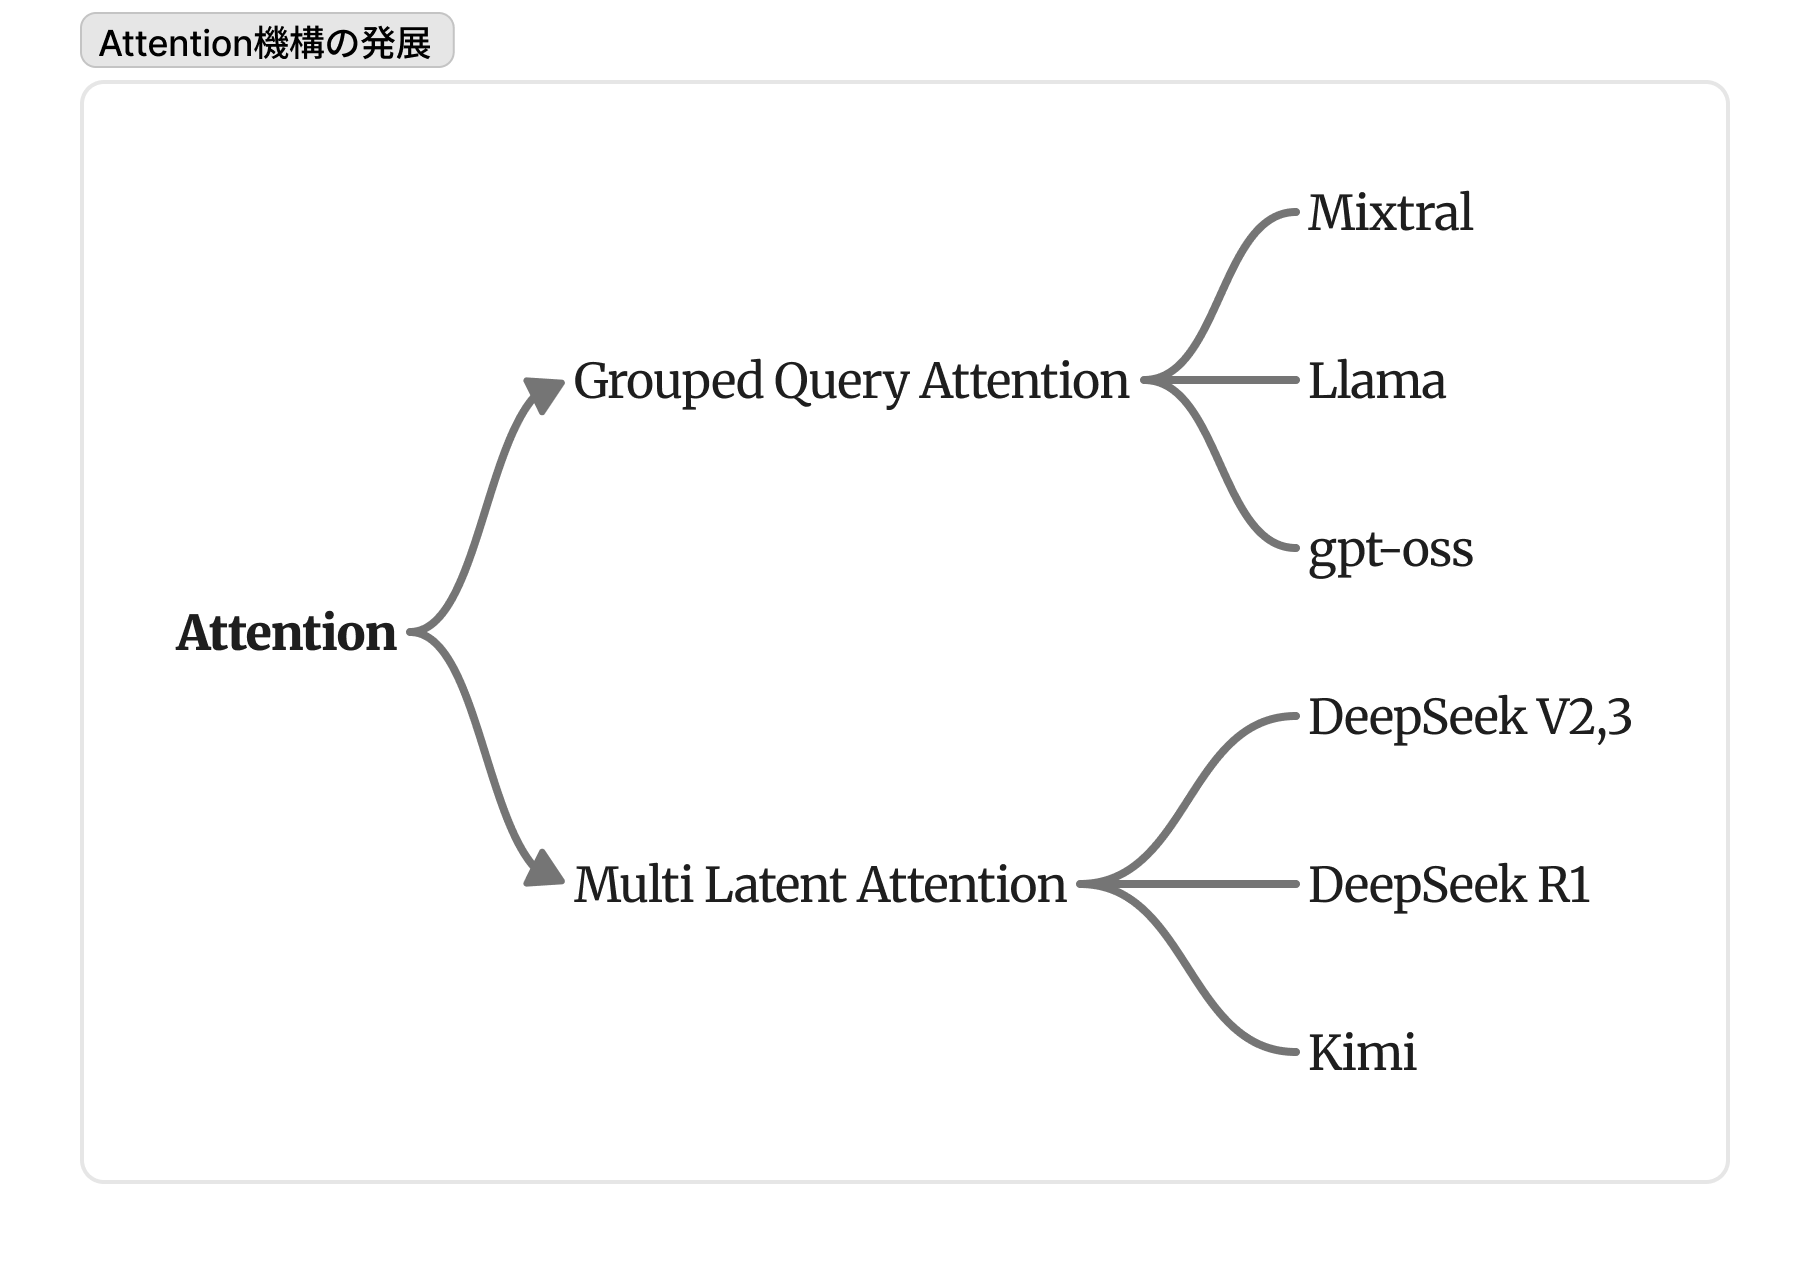
\includegraphics[width=0.8\linewidth]{Attention機構の発展.png}
    \end{figure}
    \footnotesize
    MultiheadAttentionの派生系が近年のLLMで使用される
    
    目的：性能を維持したまま計算を効率化
    
    \tiny
    \href{https://arxiv.org/abs/2305.13245}{Ainslie, J. et al., GQA: Training Generalized Multi-Query Transformer Models from Multi-Head Checkpoints, arXiv preprint arXiv:2305.13245, 2023.}
    
    \href{https://arxiv.org/abs/2405.04434}{DeepSeek-AI. et al., DeepSeek-V2: A Strong, Economical, and Efficient Mixture-of-Experts Language Model, arXiv preprint arXiv:2405.04434, 2024.}
\end{frame}

\begin{frame}{Grouped Query Attention}
    \begin{figure}[bthp]
    \centering
    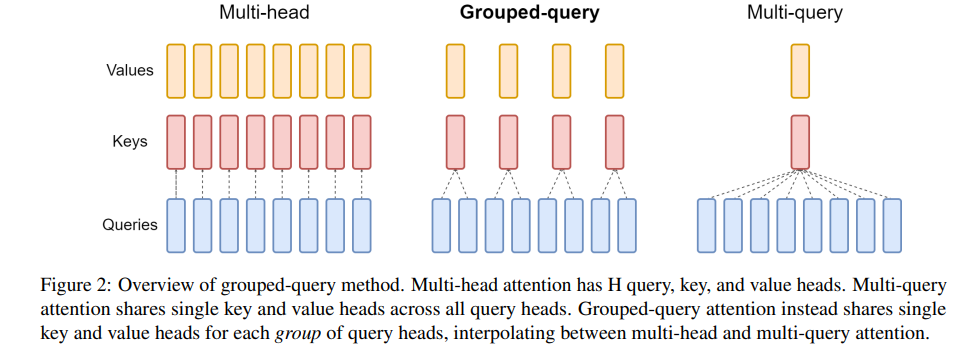
\includegraphics[width=0.7\linewidth]{MQA - GQA.png}
    \end{figure}
    \begin{columns}[c]
        \column{0.45\textwidth}
        \begin{figure}[bthp]
        \centering
        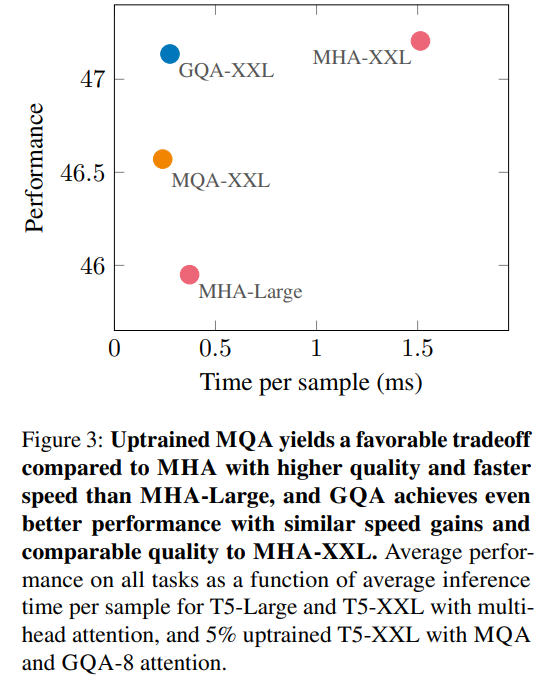
\includegraphics[width=0.8\linewidth]{GQA-MQA performance.png}
        \end{figure}

        \column{0.5\textwidth}
        \tiny
        MQA：単一のK, Vをヘッド間で共有することで推論を高速化$\rightarrow$性能低下の問題発生
        
        \vspace{1em}
        GQA：MQAとMHAの中間に位置する。MQAに近い速度とMHAに近い性能の両立が確認された
        
        \vspace{4em}
        \tiny
        \href{https://arxiv.org/abs/2305.13245}{Ainslie, J. et al., GQA: Training Generalized Multi-Query Transformer Models from Multi-Head Checkpoints, arXiv preprint arXiv:2305.13245, 2023.}
    \end{columns}
\end{frame}

\begin{frame}{Grouped Query Attention}
    \begin{figure}[bthp]
        \centering
        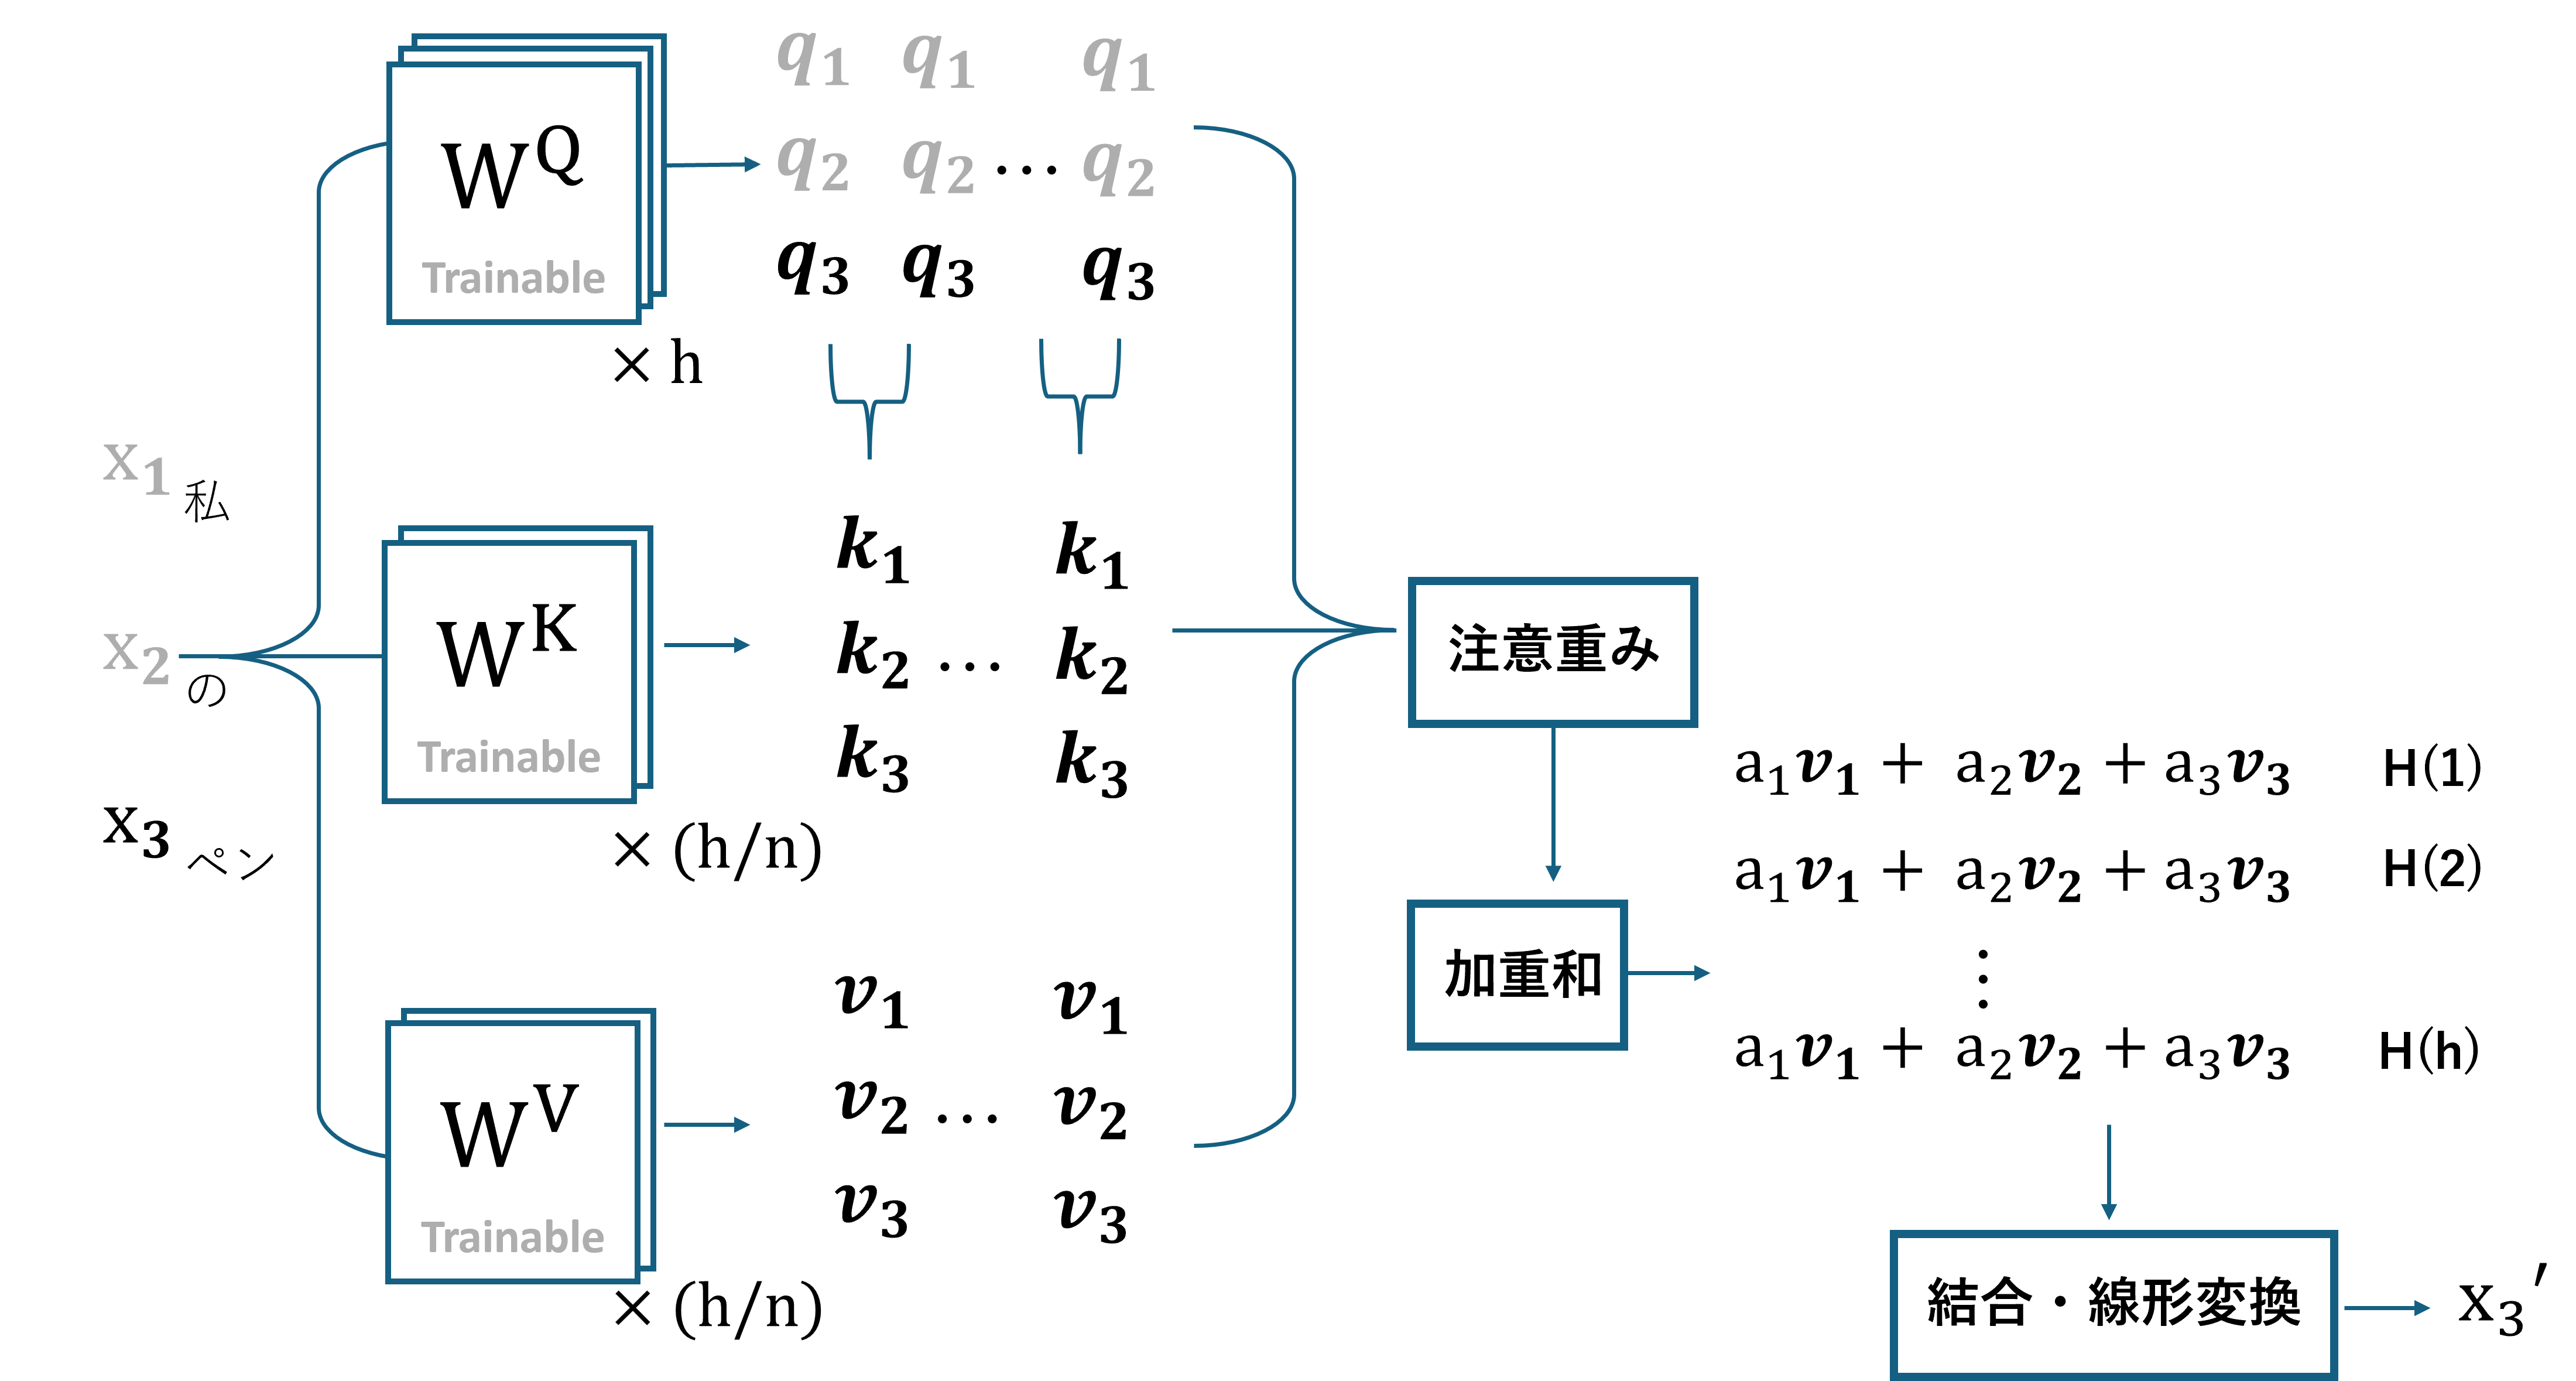
\includegraphics[width=0.8\linewidth]{Grouped Query Attention.png}
    \end{figure}

    \vspace{1em}
    \tiny
    \href{https://arxiv.org/abs/2305.13245}{Ainslie, J. et al., GQA: Training Generalized Multi-Query Transformer Models from Multi-Head Checkpoints, arXiv preprint arXiv:2305.13245, 2023.}
\end{frame}

\begin{frame}{Multi-head Latent Attention}
    \begin{figure}[bthp]
    \centering
    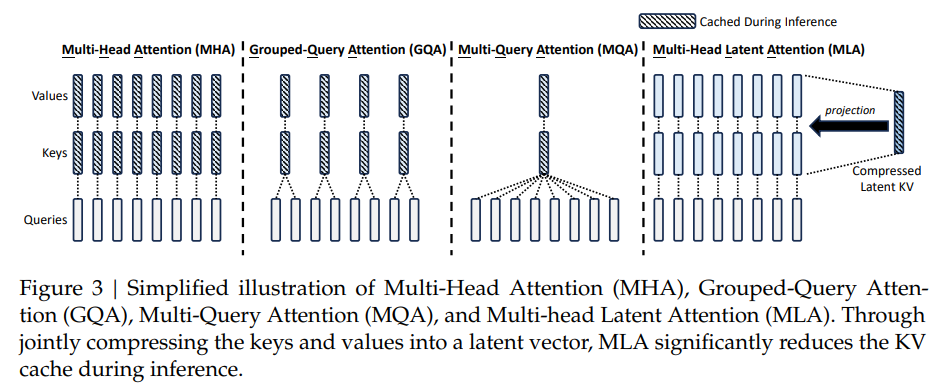
\includegraphics[width=0.8\linewidth]{Multi-head Latent Attention.png}
    \end{figure}
    
    \tiny
    \href{https://arxiv.org/abs/2405.04434}{DeepSeek-AI. et al., DeepSeek-V2: A Strong, Economical, and Efficient Mixture-of-Experts Language Model, arXiv preprint arXiv:2405.04434, 2024.}
\end{frame}

\begin{frame}{Multi-head Latent Attention}
    \begin{figure}[bthp]
    \centering
    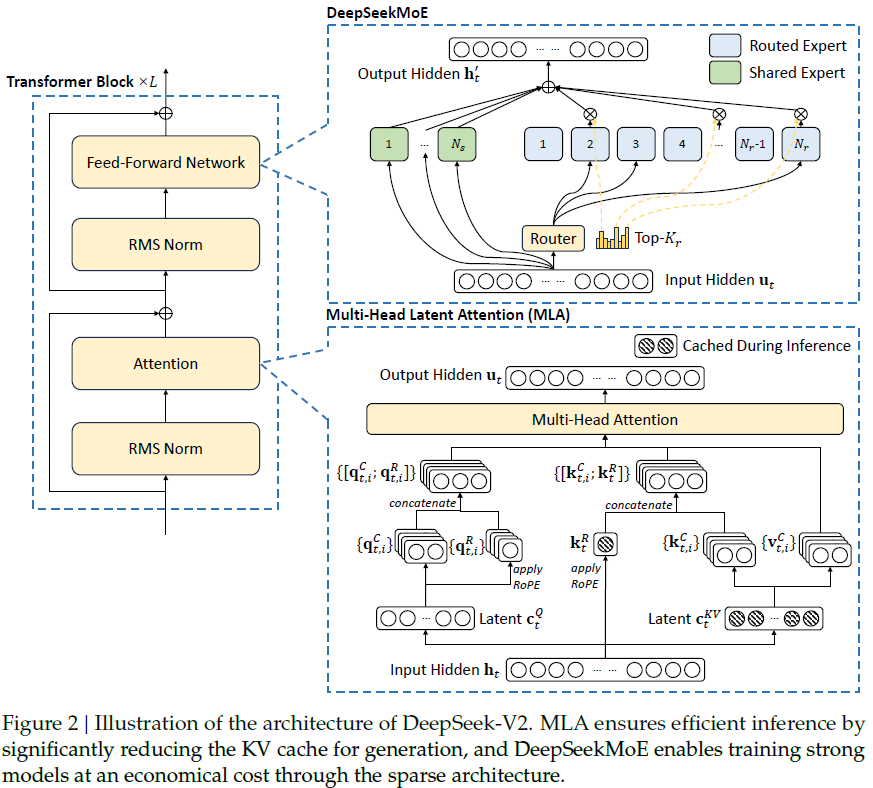
\includegraphics[width=0.8\linewidth]{Multi-head Latent Attention fig2.png}
    \end{figure}
    
    \tiny
    \href{https://arxiv.org/abs/2405.04434}{DeepSeek-AI. et al., DeepSeek-V2: A Strong, Economical, and Efficient Mixture-of-Experts Language Model, arXiv preprint arXiv:2405.04434, 2024.}
\end{frame}

\begin{frame}{Multi-head Latent Attention}
    \begin{figure}[bthp]
        \centering
        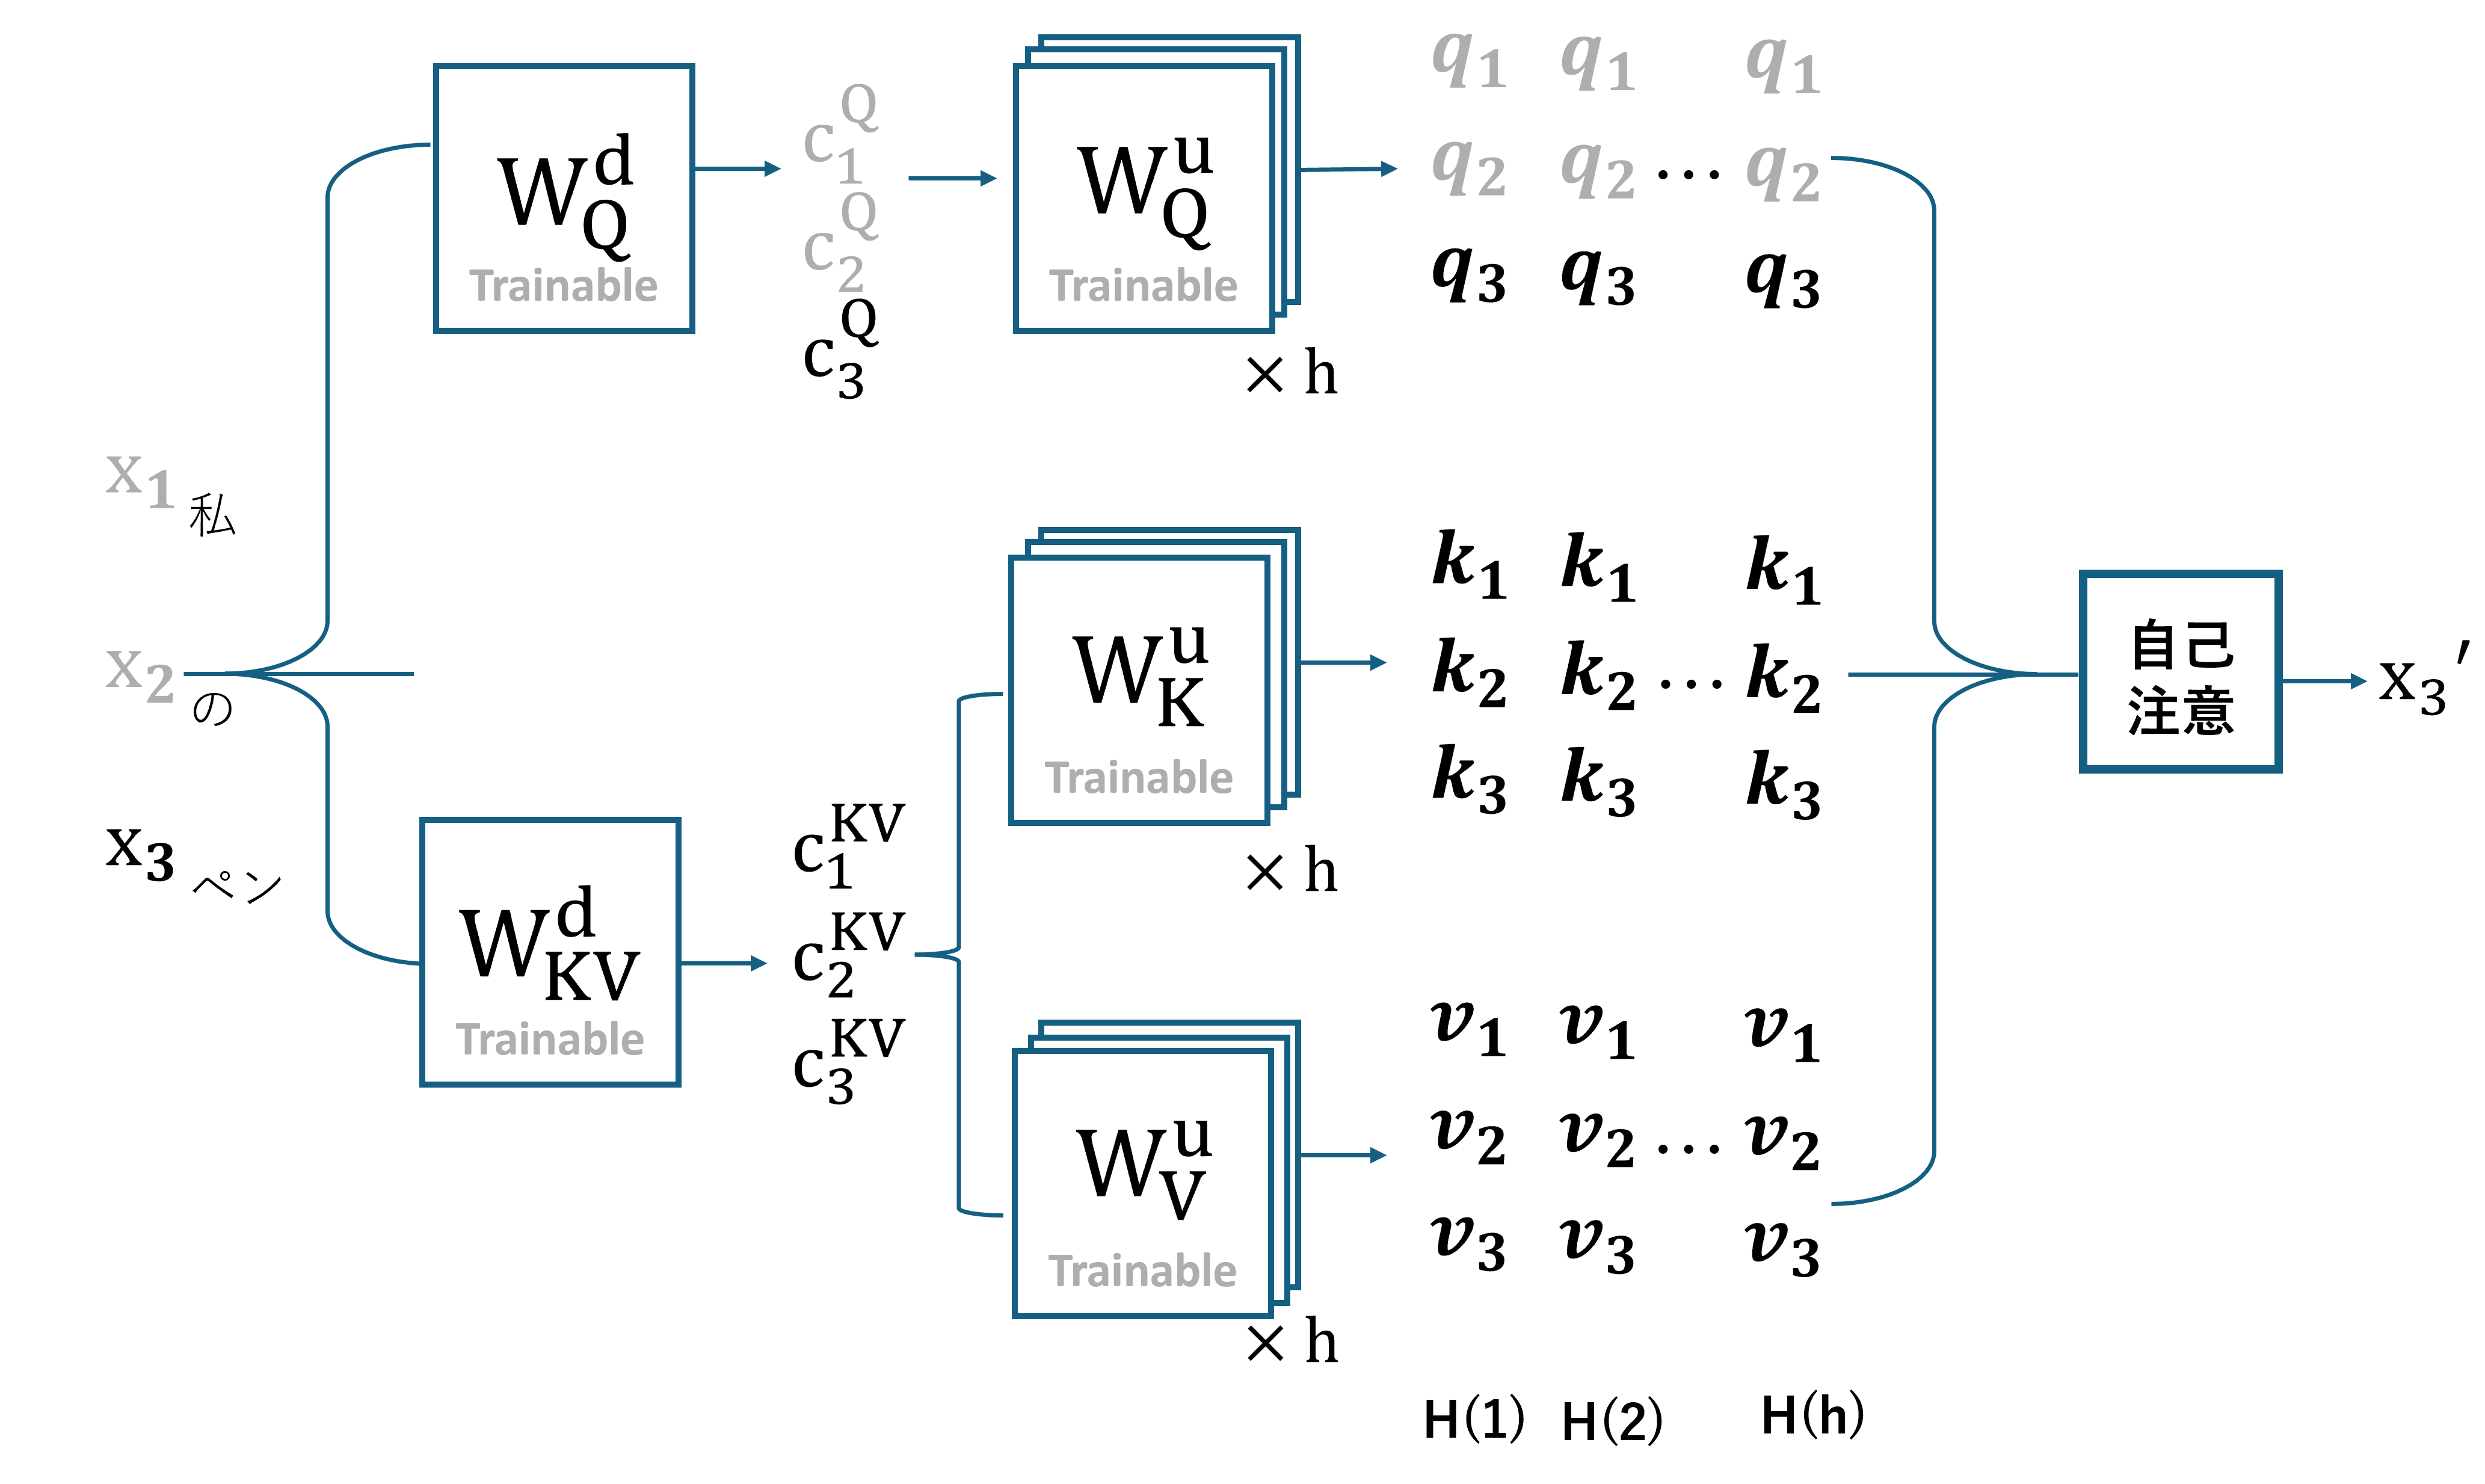
\includegraphics[width=0.8\linewidth]{Multi-head Latent Attention 1.png}
    \end{figure}

    \vspace{1em}
    \tiny
    \href{https://arxiv.org/abs/2405.04434}{DeepSeek-AI. et al., DeepSeek-V2: A Strong, Economical, and Efficient Mixture-of-Experts Language Model, arXiv preprint arXiv:2405.04434, 2024.}
\end{frame}

\begin{frame}{どの文脈情報を参照しているか}
    \begin{figure}[bthp]
    \centering
    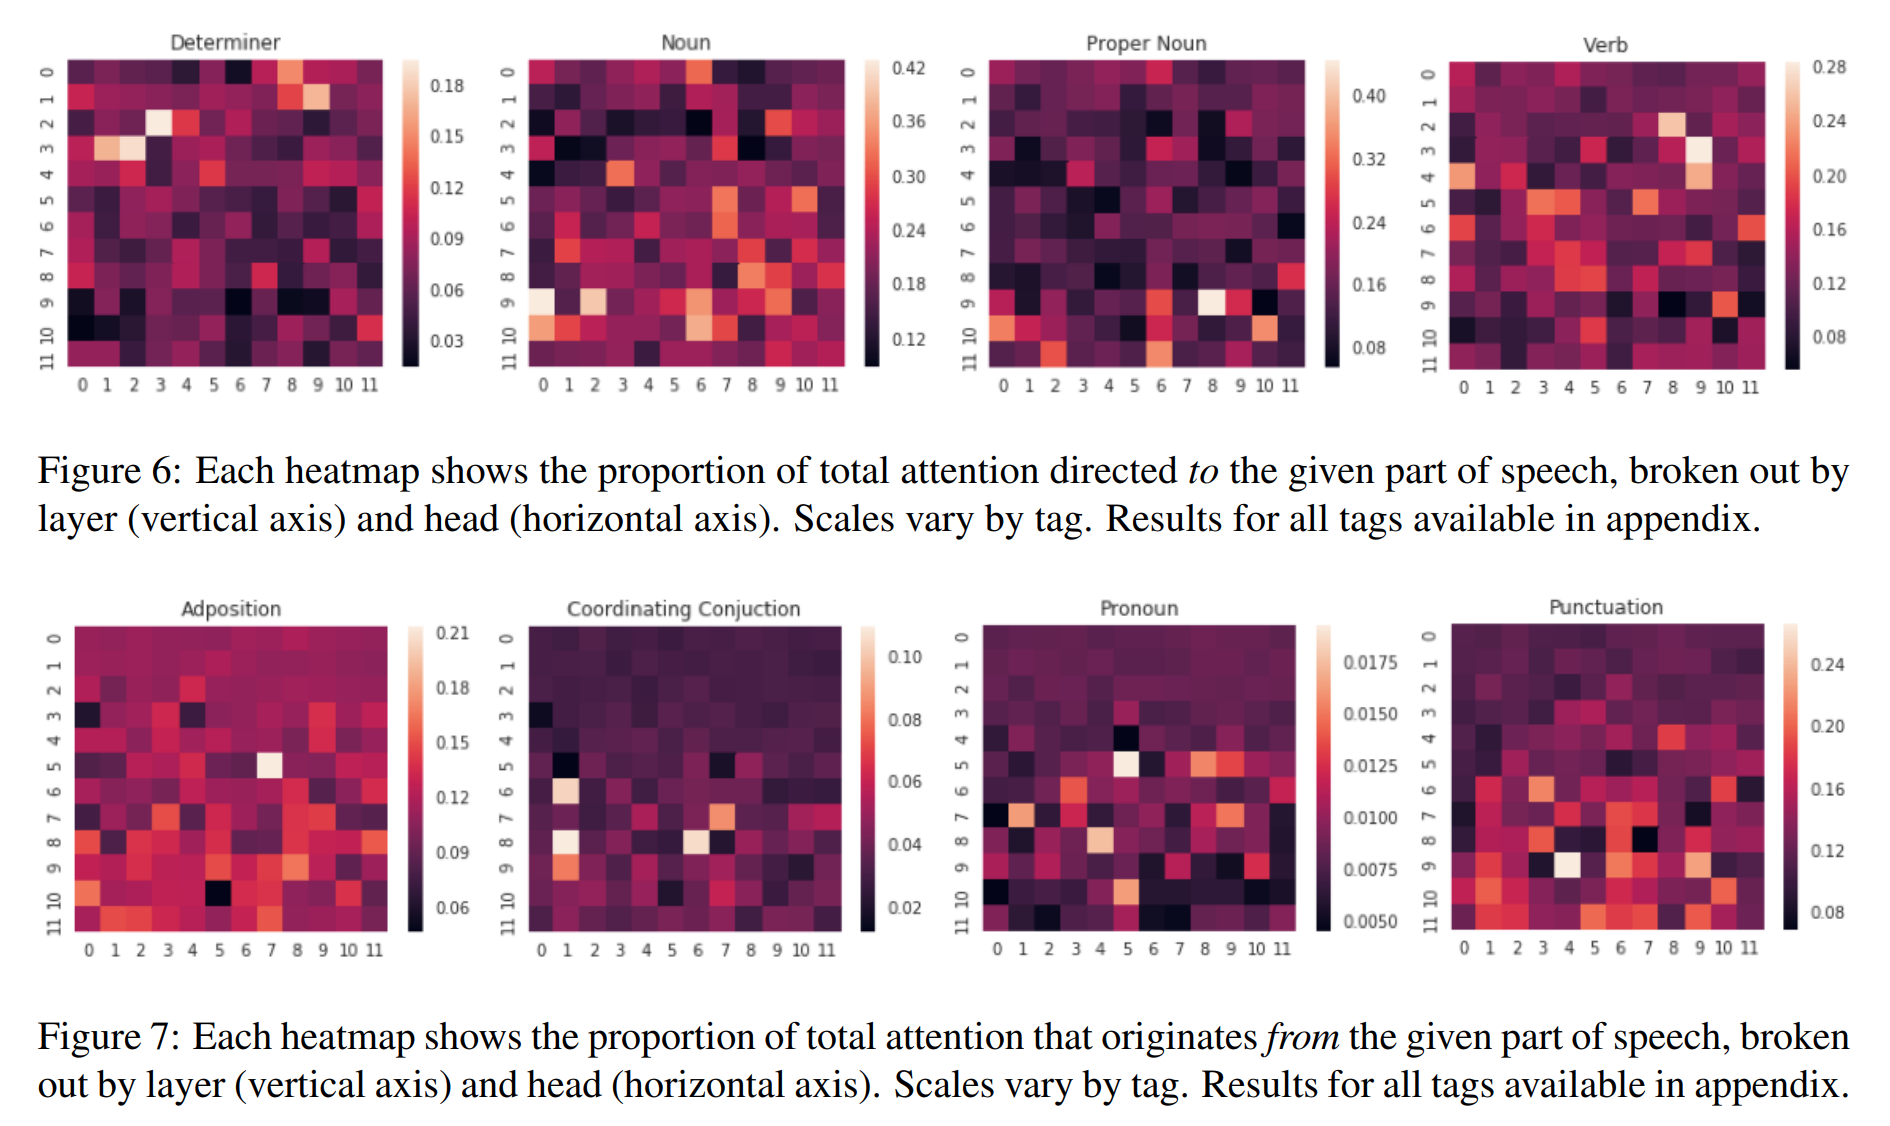
\includegraphics[width=1\linewidth]{Attention Layer-Head.png}
    \end{figure}
    \footnotesize
    特定の品詞(名詞・動詞など)を強く参照するヘッドが存在する

    \tiny
    \href{https://arxiv.org/abs/1906.04284}{Vig, J. and Belinkov, Y., Analyzing the Structure of Attention in a Transformer Language Model, arXiv preprint arXiv:1906.04284, 2019.}
\end{frame}

\begin{frame}{Local Attention・Global Attention}
    \begin{columns}[c]
        \column{0.45\textwidth}
        \begin{figure}[bthp]
        \centering
        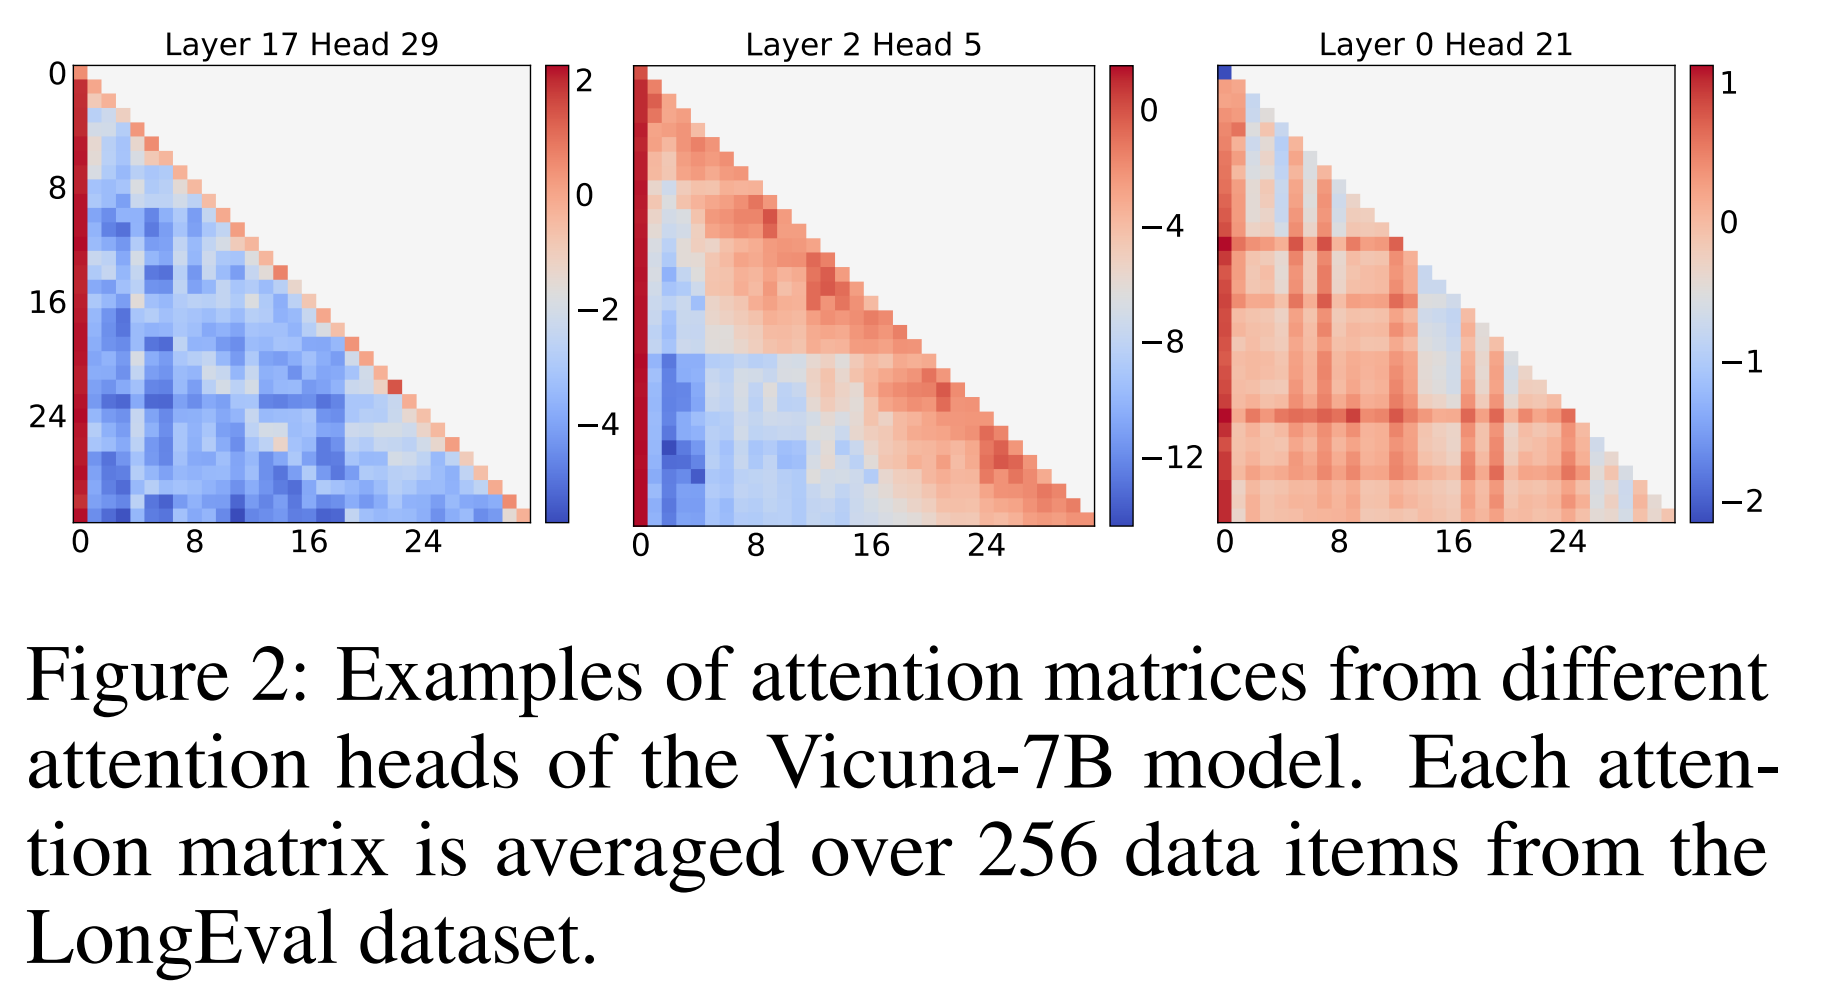
\includegraphics[width=1\linewidth]{Local - Global Attention.png}
        \end{figure}

        \column{0.5\textwidth}
        \begin{itemize}
            \item 近くの情報を参照する(Local Attention)
            \begin{itemize}
                \item 隣接する数トークンを強く参照するヘッドが多く存在する
            \end{itemize}
            \item 文脈を広く参照する(Global Attention)
            \begin{itemize}
                \item 入力に応じて文脈を広く参照するヘッドが存在する
            \end{itemize}
        \end{itemize}
    \end{columns}
    \vspace{5em}
    \tiny
    \href{https://openreview.net/forum?id=konDsSUSqg}{Fu, T. et al., MoA: Mixture of Sparse Attention for Automatic Large Language Model Compression, 2025.}
\end{frame}

\section{計算過程の解釈・解析について}
\begin{frame}{Mechanistic Interpretability}
    \begin{itemize}
        \item AIの内部構造を解明し, 安全性や価値の整合性を確保するために重要
        \item ニューラルネットワークが学習した計算メカニズムを人間が理解可能な形に改正し, 詳細かつ因果的な理解を目指す
    \end{itemize}
\end{frame}

\begin{frame}{Mechanistic Interpretability}
    \begin{itemize}
        \item \textcolor{cyan}{観察的手法}
        \begin{itemize}
            \item プローブ
            \item Logit lens
            \item Sparse Auto Encoder
        \end{itemize}
        \item 介入的手法
        \begin{itemize}
            \item Active Patching
            \item Causal Abstraction 
            \item Hypothesis Testiong
        \end{itemize}
    \end{itemize}
\end{frame}

\begin{frame}{プローブ}
    \begin{columns}[c]
        \column{0.5\textwidth}
        \begin{figure}[bthp]
            \centering
            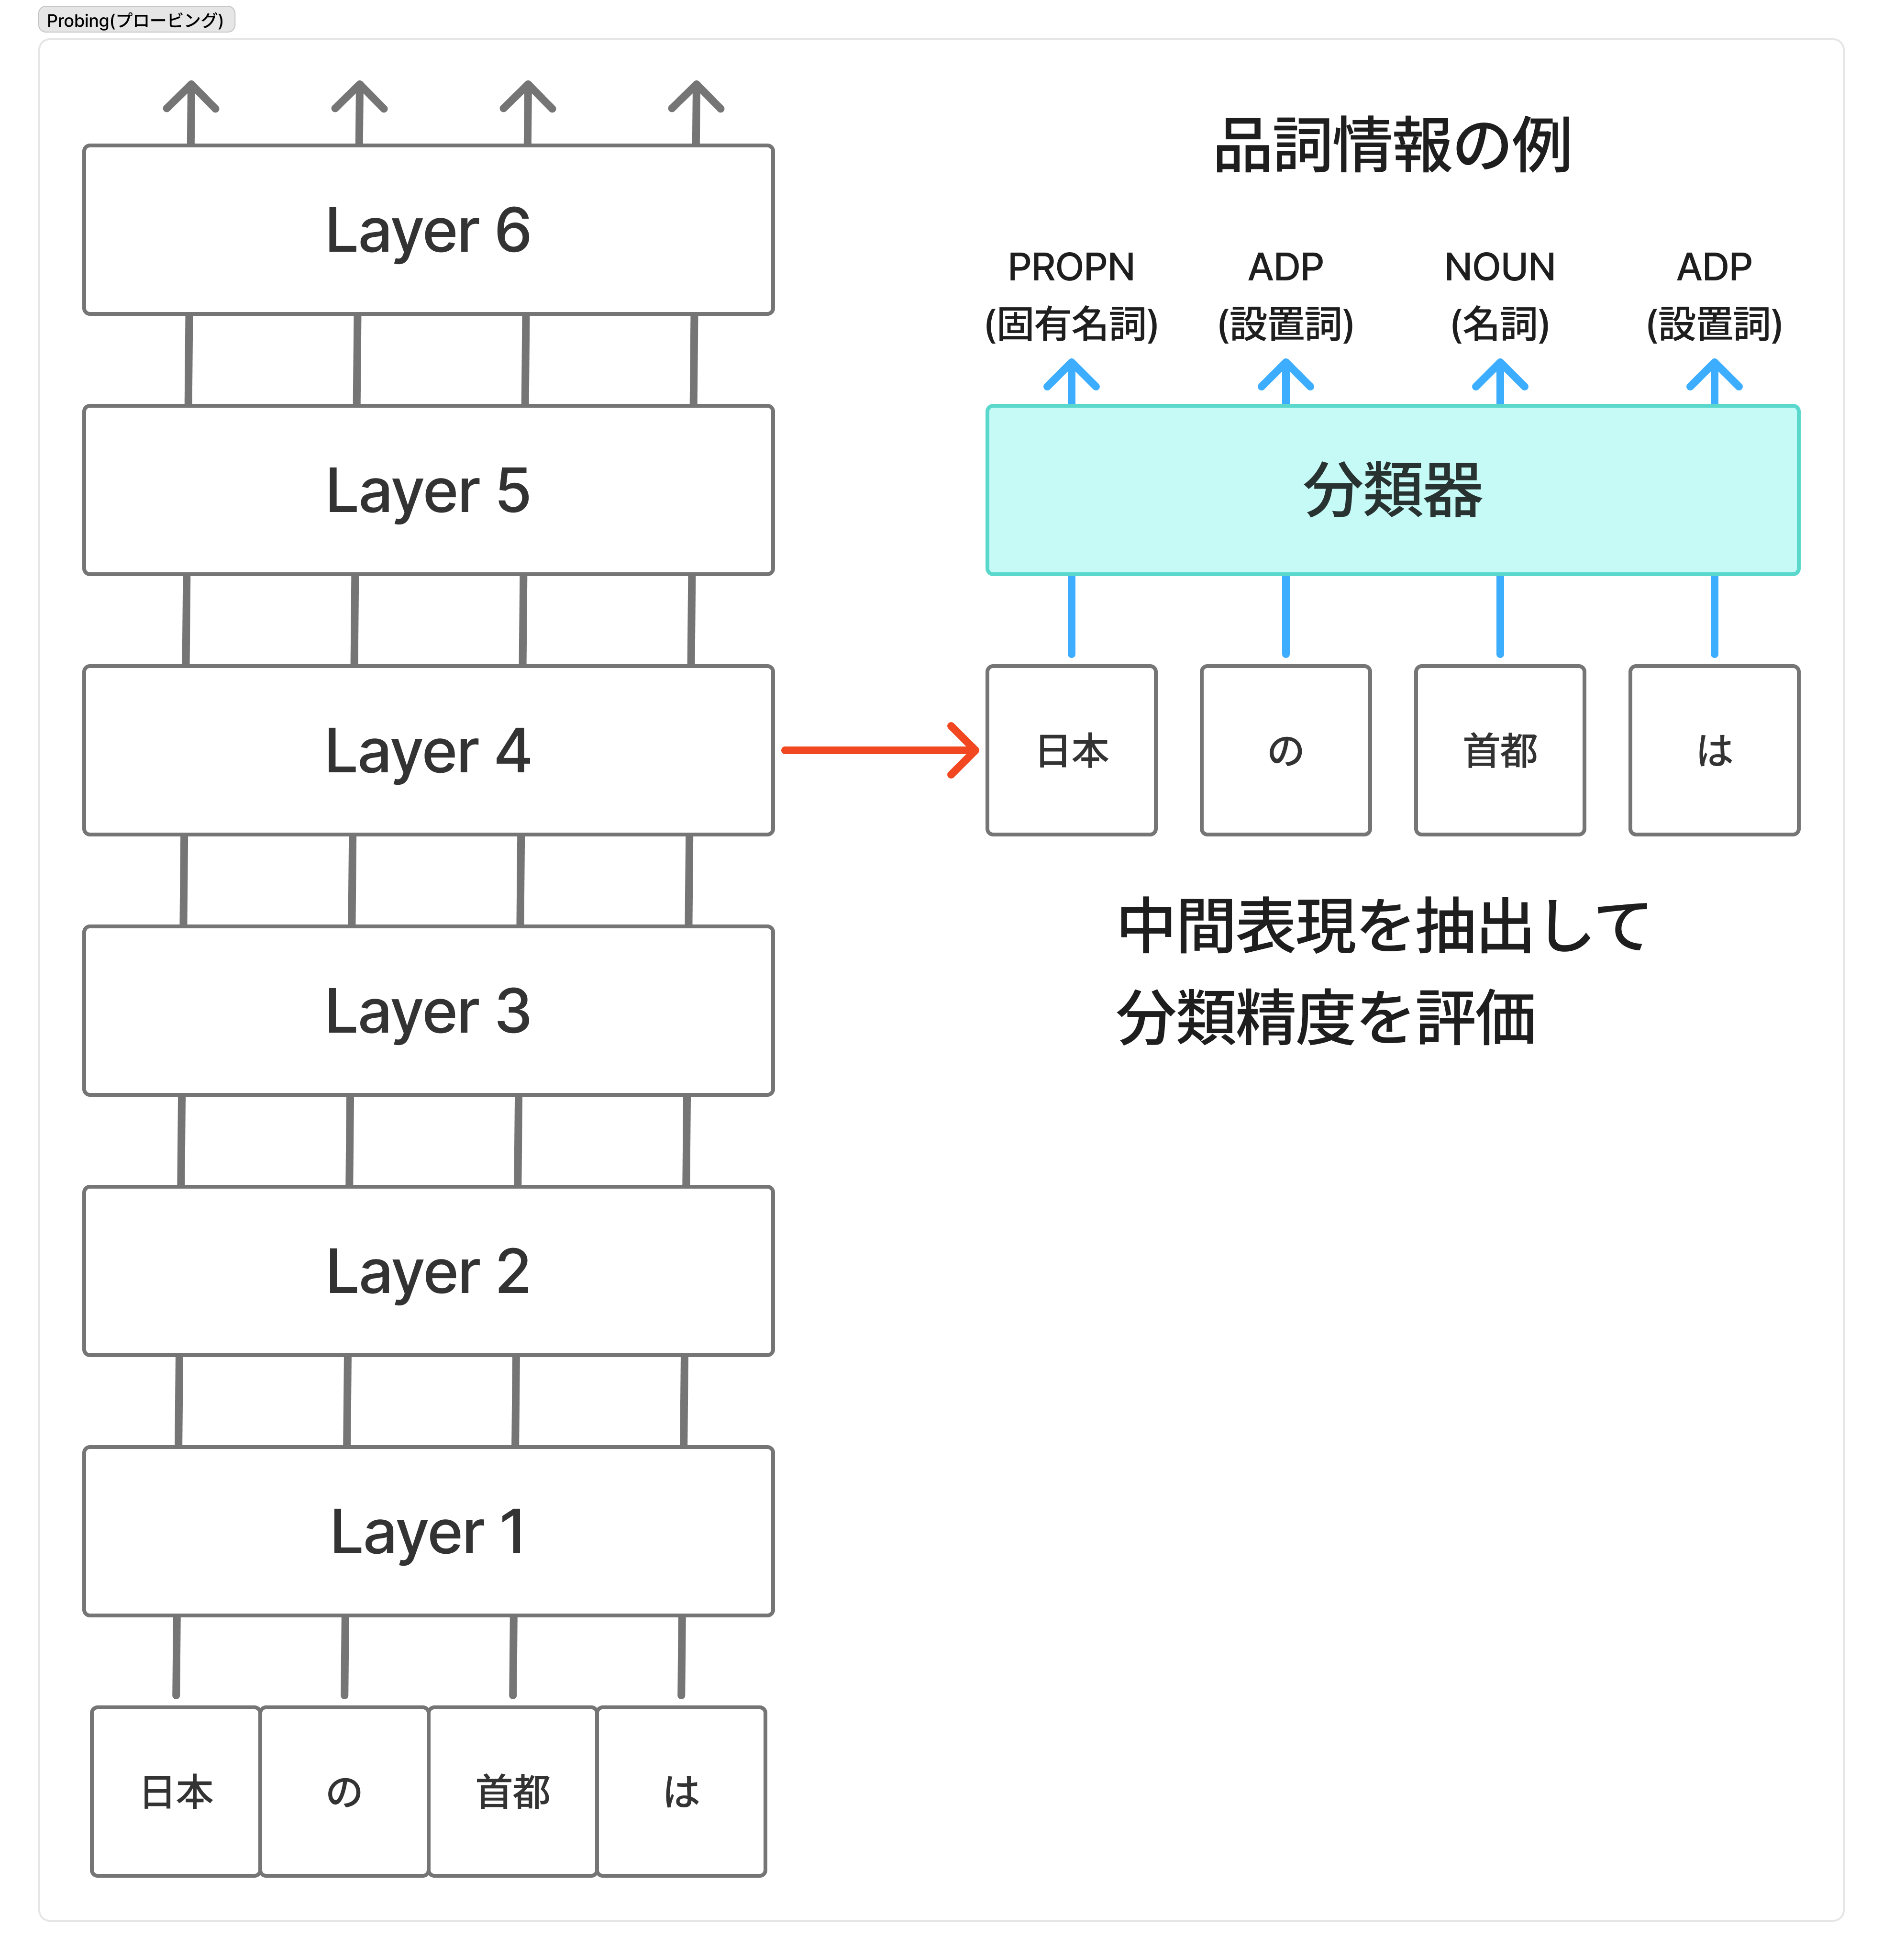
\includegraphics[width=1\linewidth]{Probing品詞タギング.png}
        \end{figure}
        \column{0.5\textwidth}
        \begin{figure}[bthp]
            \centering
            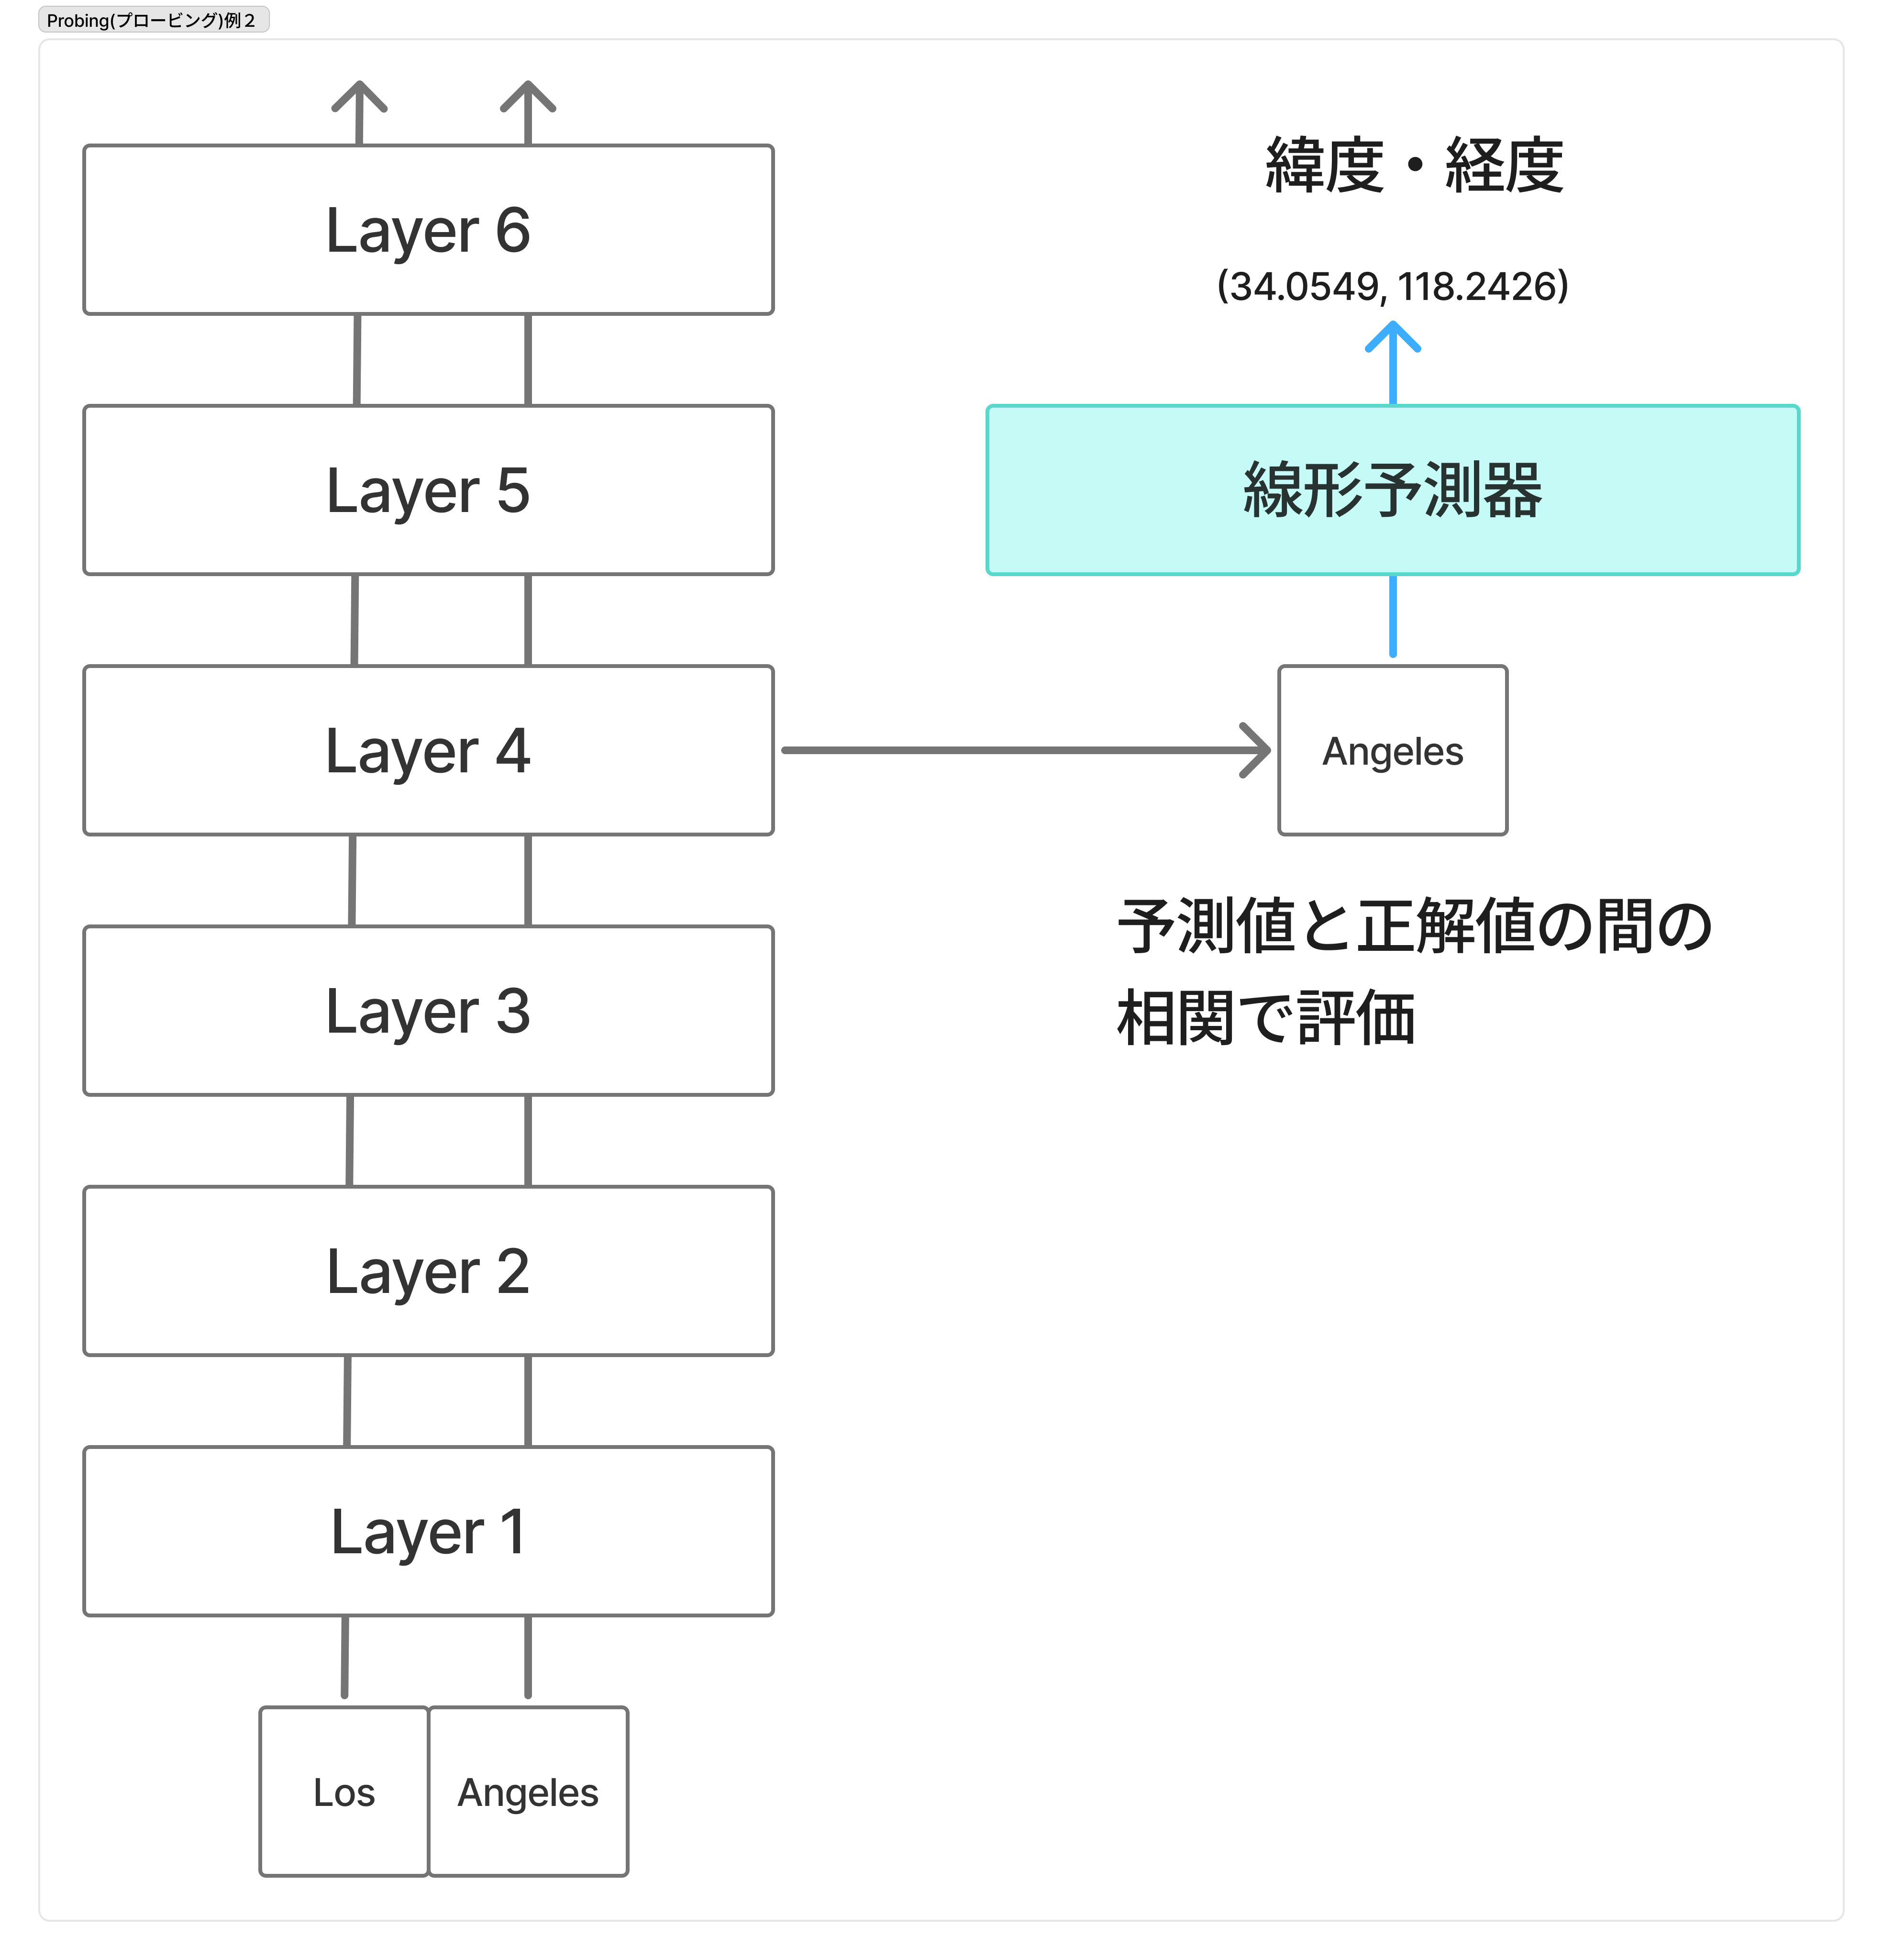
\includegraphics[width=1\linewidth]{Probing 緯度経度.png}
        \end{figure}
    \end{columns}
\end{frame}

\begin{frame}{緯度経度のプローブ}
    \begin{figure}[bthp]
        \centering
        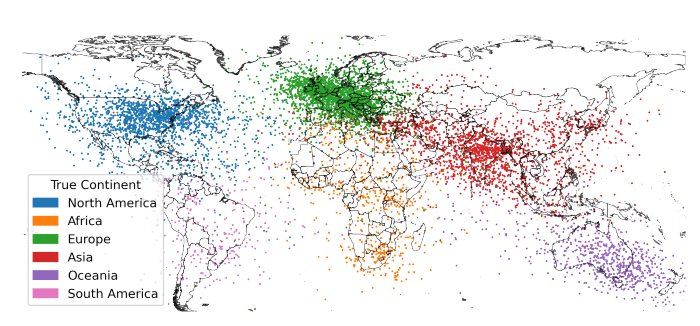
\includegraphics[width=1\linewidth]{緯度経度のプローブ.png}
    \end{figure}
    \begin{itemize}
        \item 地名を表すモデル表現から地理座標をプローブ
        \item →地理座標はおそらくエンコードされている
    \end{itemize}
    \vspace{2em}
    \tiny
    \href{https://arxiv.org/abs/2310.02207}{Gurnee, W. and Tegmark, M., Language Models Represent Space and Time, ICLR, 2024.}
\end{frame}

\begin{frame}{Logit lens}
    \begin{columns}[c]
        \column{0.5\textwidth}
        \begin{figure}[bthp]
            \centering
            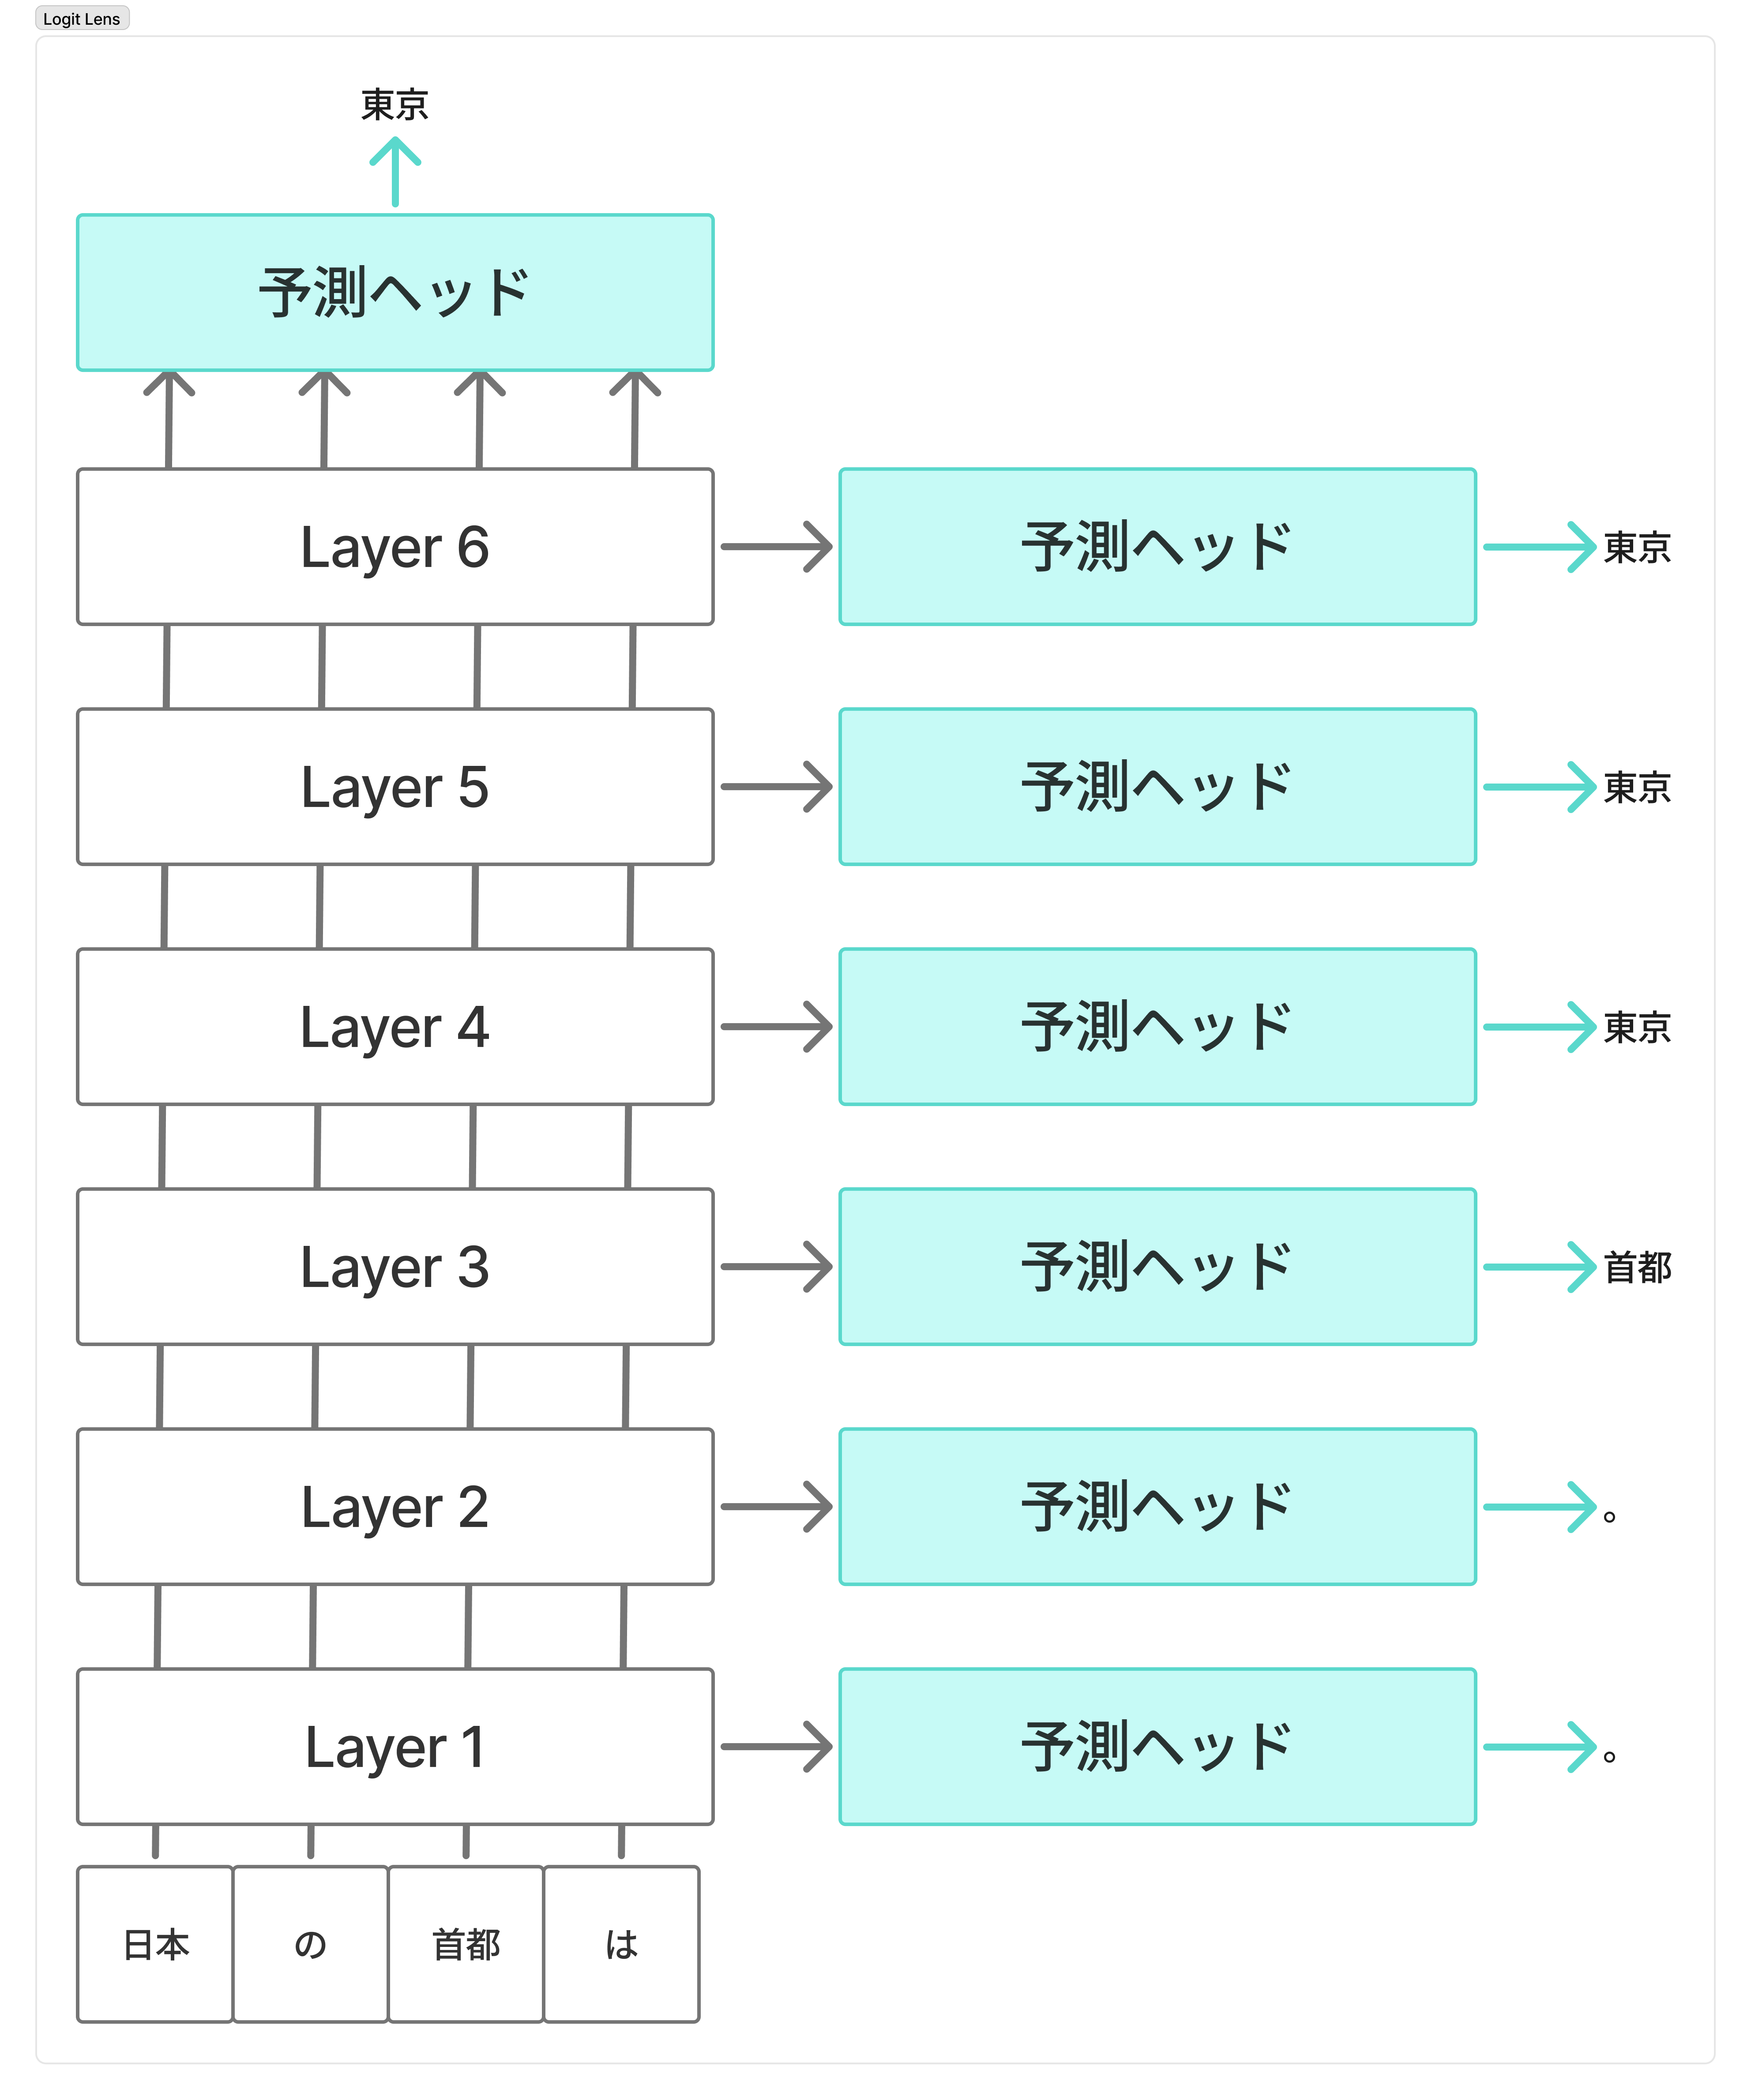
\includegraphics[width=1\linewidth]{Logit Lens.png}
        \end{figure}
        \column{0.5\textwidth}
        \tiny
        各層の中間表現を予測ヘッドに渡して語彙に紐づける
        モデル各層を通して予測がどう進んでいったか追うことが可能
    \end{columns}
    \vspace{1em}
    \tiny
    \href{https://arxiv.org/abs/2209.02535}{Dar, G. et al., Analyzing Transformers in Embedding Space, arXiv preprint arXiv:2209.02535, 2022.}
\end{frame}

\begin{frame}{PolysemanticityとSuperposition}
    Polysemanticity(多義性)
    \begin{itemize}
        \item 1つのニューロンが意味的に異なる複数の入力に発火する現象
        \item \rightarrow 解釈しづらい
    \end{itemize}
    Superposition(重ね合わせ)
    \begin{itemize}
        \item あまり登場しないレアな概念を少数のニューロンに圧縮することで, モデルがレイヤーの次元数よりも多くの特徴量を学習できるという仮説
        \item 重ね合わせによってPolysemanticityが起きているのではと考えられている
    \end{itemize}
    \vspace{3em}
    \tiny
    \url{https://transformer-circuits.pub/2022/toy_model/index.html} (2022)
\end{frame}

\begin{frame}{Sparse Auto Encoder: SAE}
    \begin{figure}[bthp]
    \centering
    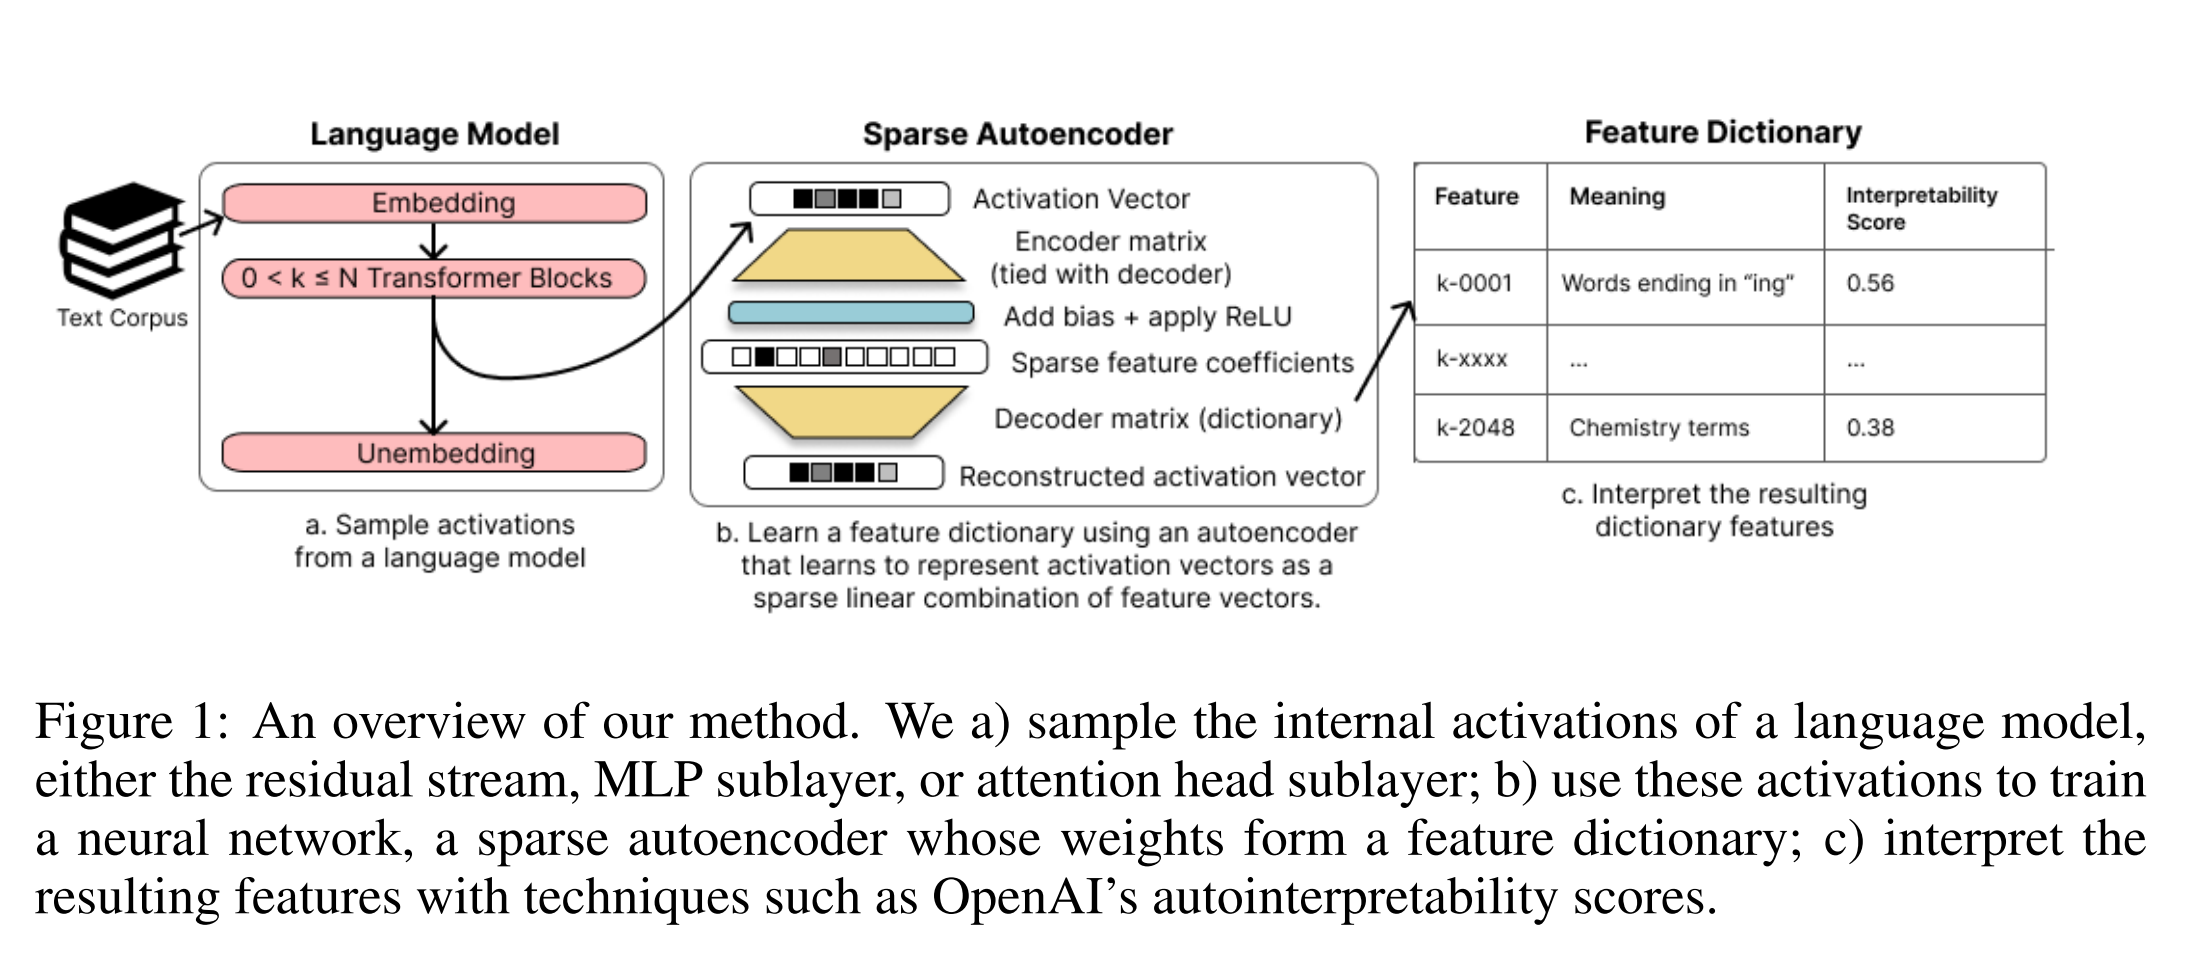
\includegraphics[width=1\linewidth]{Sparse Auto Encoder.png}
    \end{figure}
    \vspace{5em}
    \tiny
    \href{https://arxiv.org/abs/2309.08600}{Cunningham, H. et al., Sparse Autoencoders Find Highly Interpretable Features in Language Models, arXiv preprint arXiv:2309.08600, 2023.}
\end{frame}

\begin{frame}{Sparse Auto Encoder: SAE}
    \begin{columns}[c]
        \column{0.5\textwidth}
        \begin{figure}[bthp]
        \centering
        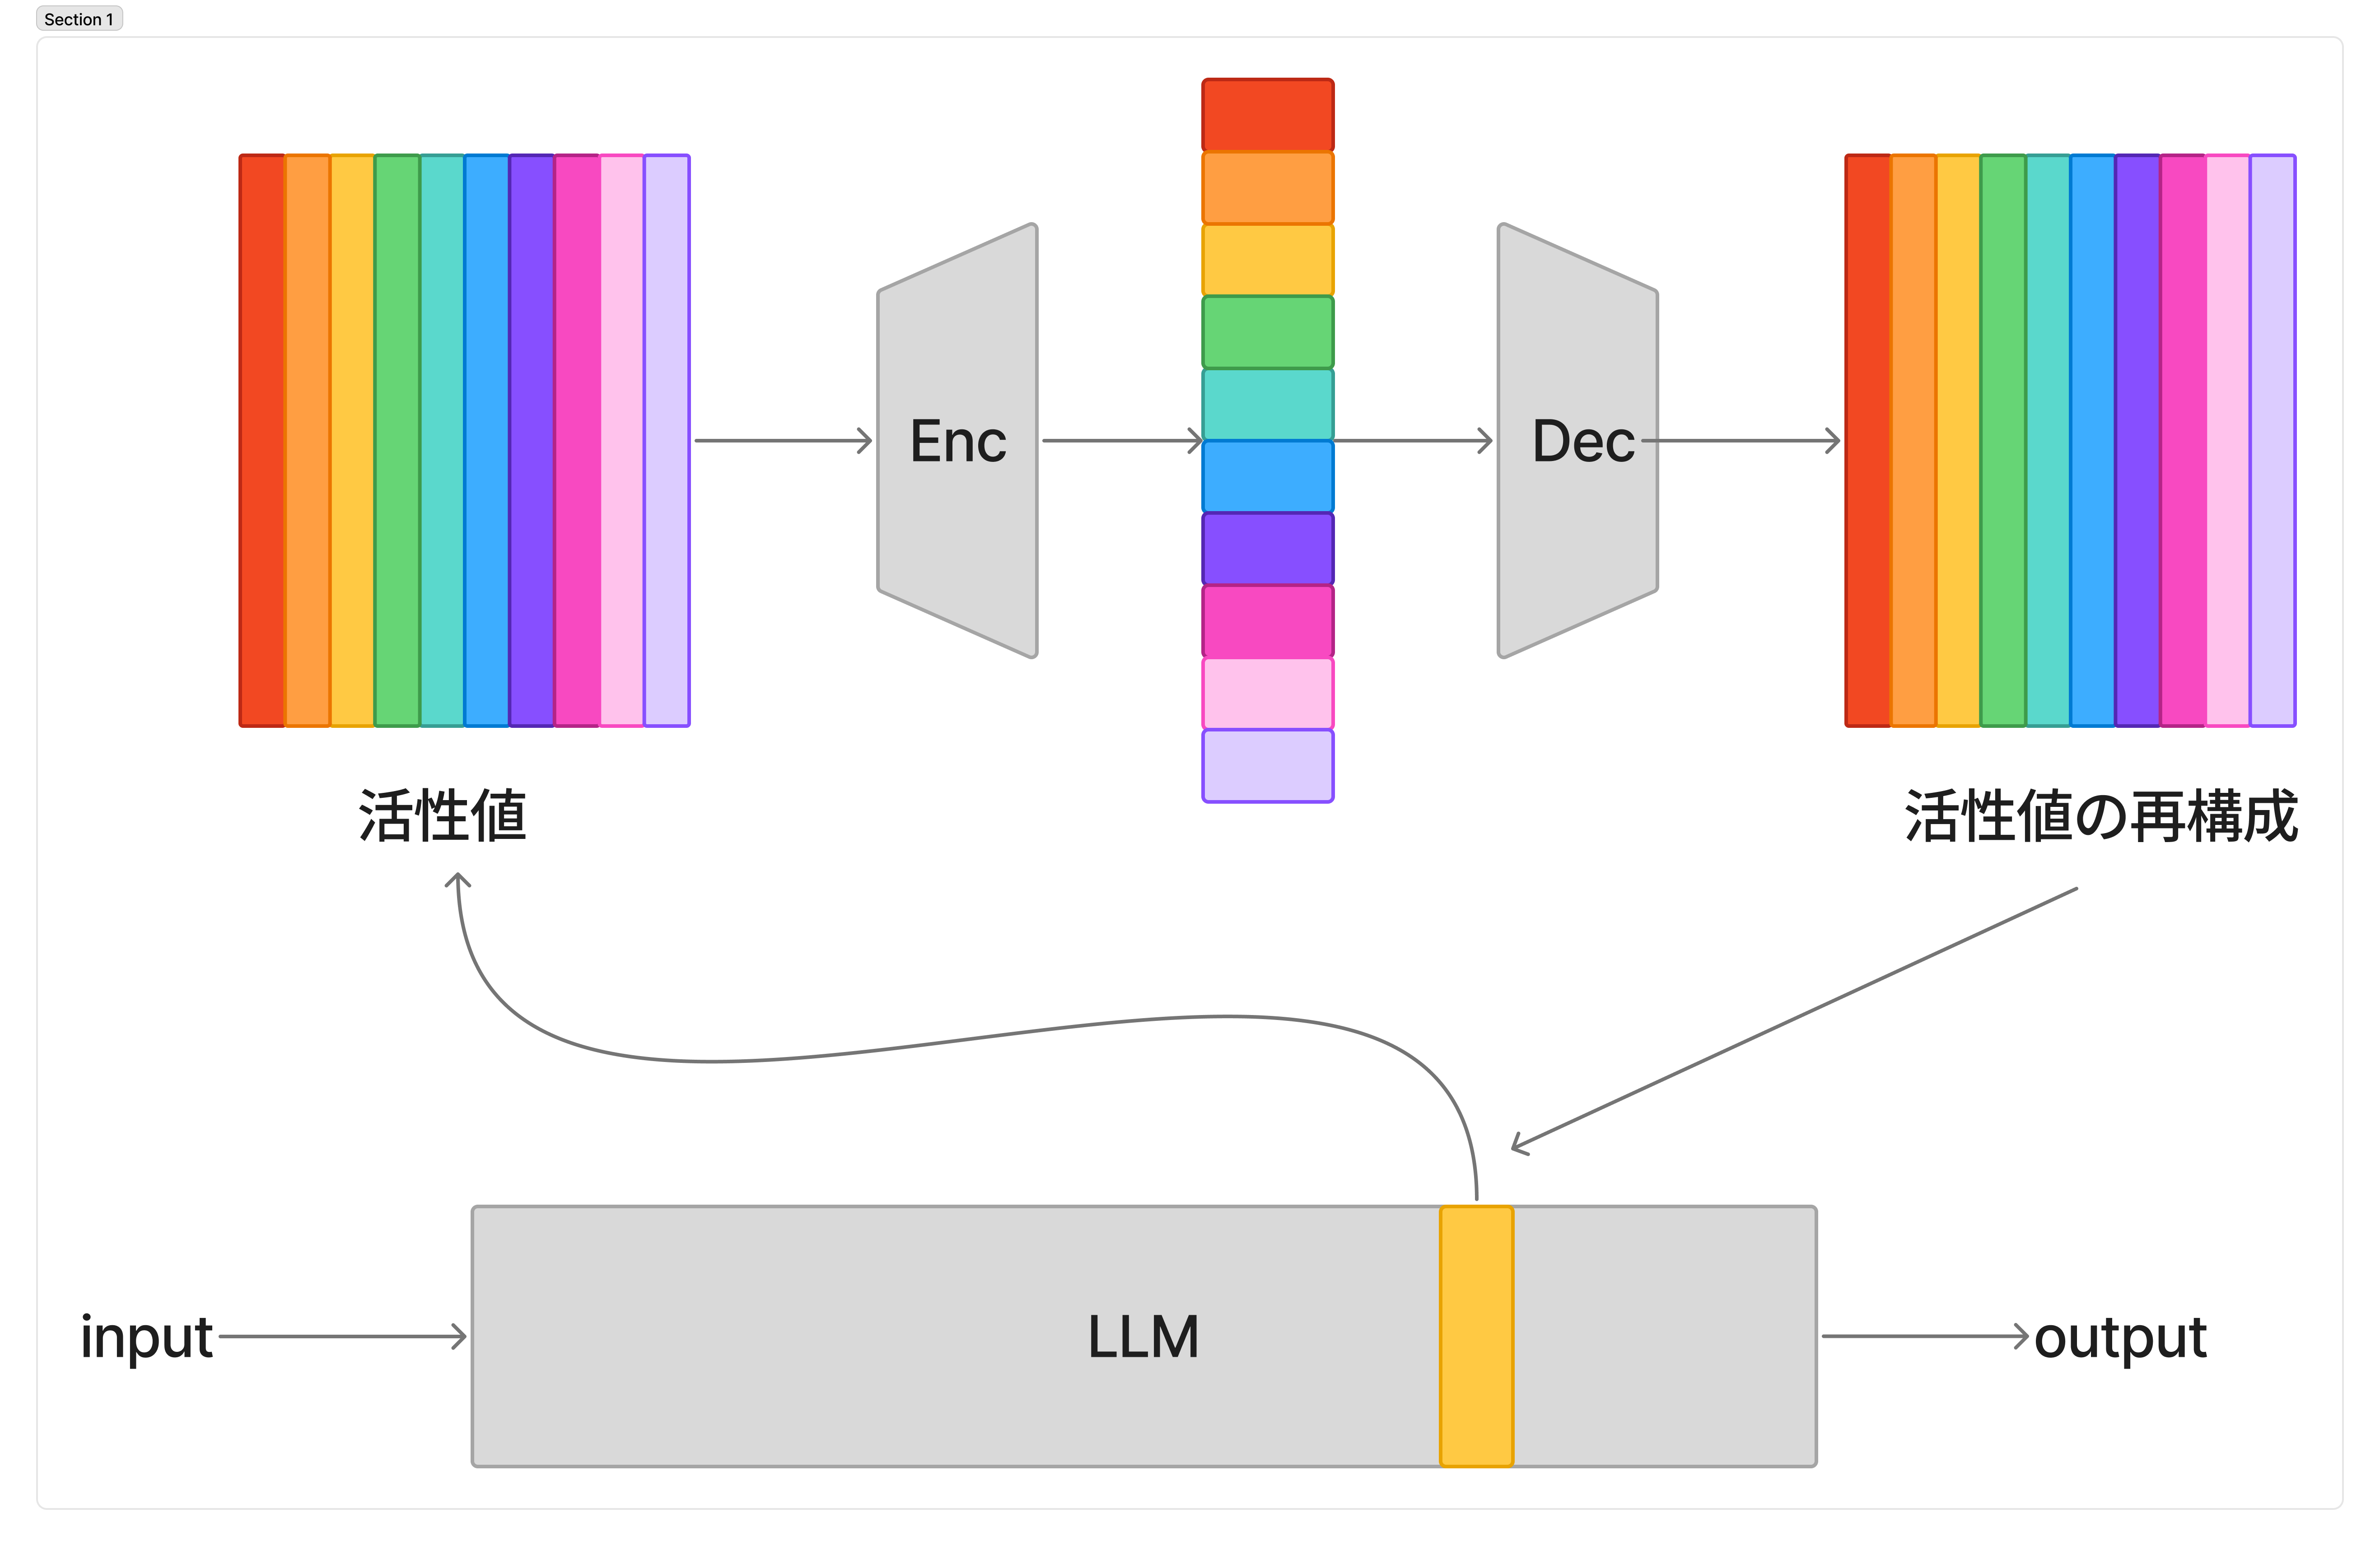
\includegraphics[width=1\linewidth]{SAE略図.png}
        \end{figure}
        \column{0.45\textwidth}
        \begin{figure}[bthp]
        \centering
        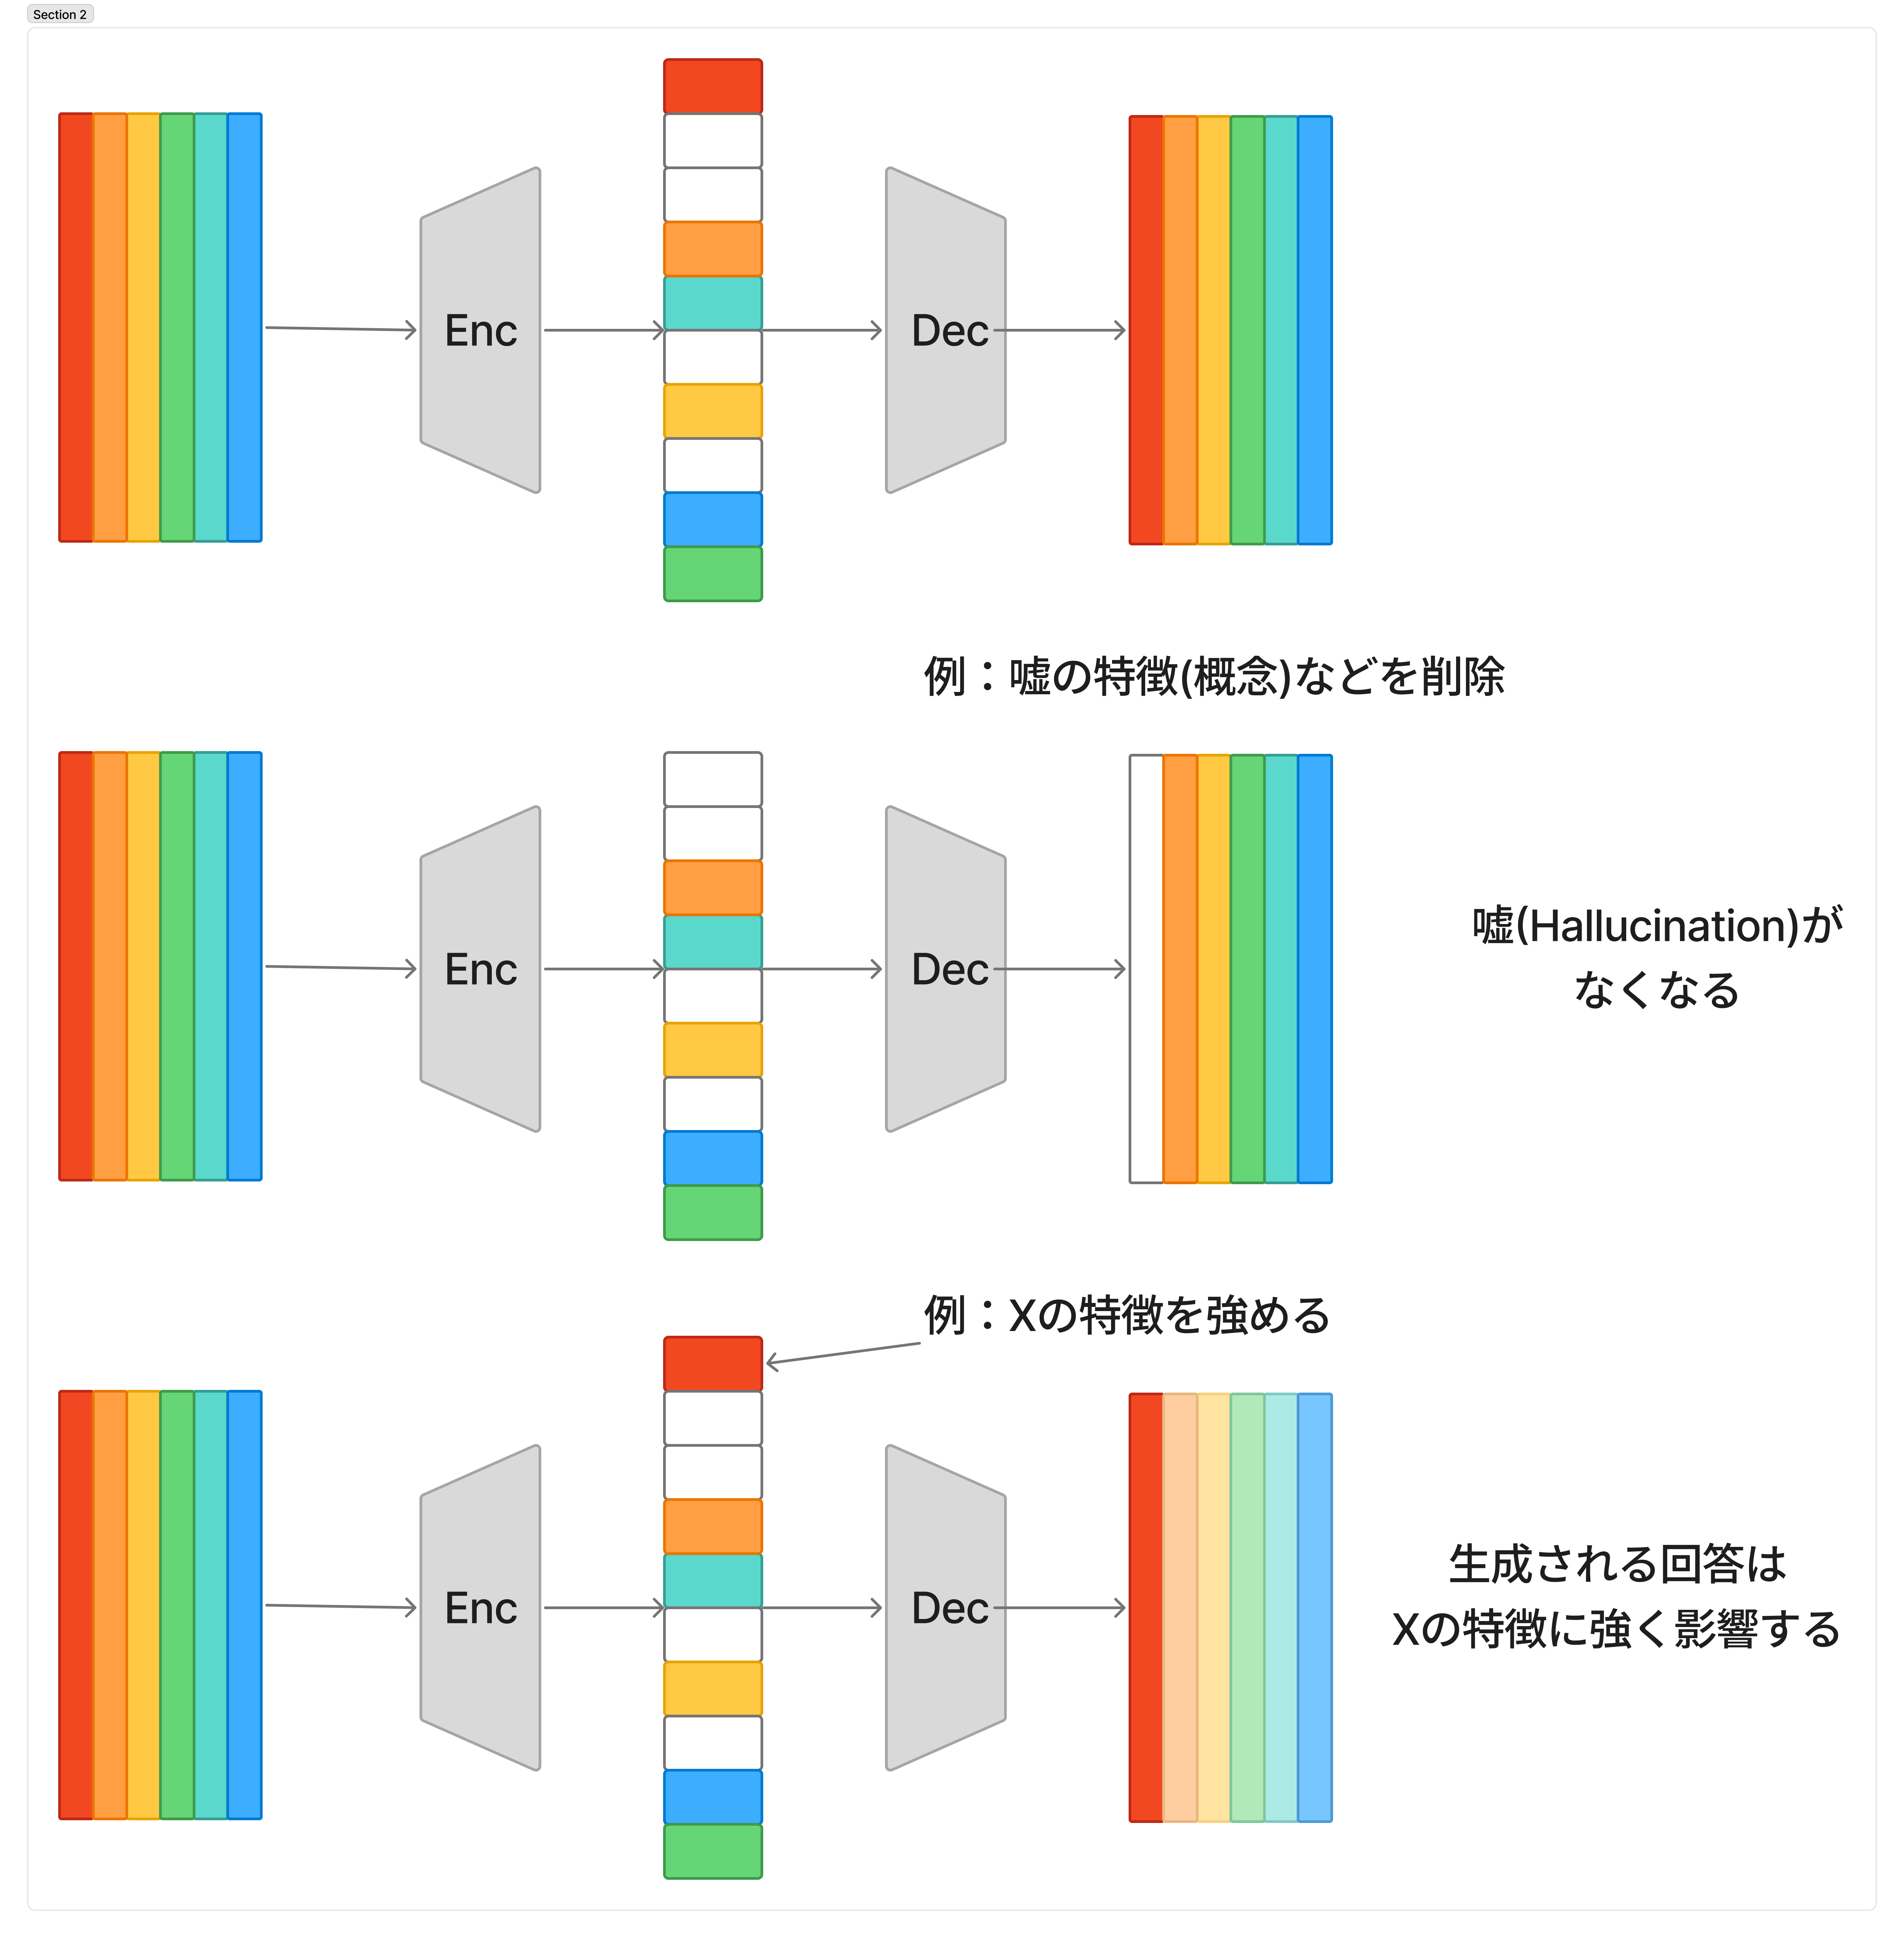
\includegraphics[width=1\linewidth]{SAE略図具体例.png}
        \end{figure}
    \end{columns}
\end{frame}

\begin{frame}{SAEによる特徴抽出過程}
    \begin{columns}[T]
        \column{0.35\textwidth}
        \begin{figure}[bthp]
        \centering
        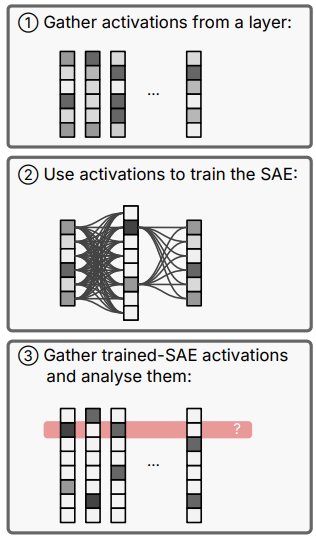
\includegraphics[width=1\linewidth]{SAE_process.png}
        \end{figure}
        
        \column{0.65\textwidth}
        \begin{enumerate}\scriptsize 
            \item \textbf{LLM内部activationを収集}
            \begin{itemize}\scriptsize 
                \item 多様なテキストをLLMへ入力
                \item 特定layerのactivationを集める
                \item 例：MLP activation（活性化関数後）
            \end{itemize}
            \item \textbf{SAEを学習}
            \begin{itemize}\scriptsize 
                \item activationを高次元空間へ射影
                \item sparsity制約により少数featureのみ活性化
                \item sparse featureの組み合わせから元activationを再構成
            \end{itemize}
            \item \textbf{featureを解析}
            \begin{itemize}\scriptsize 
                \item 学習済みSAEでactivationをfeatureへ分解
                \item 各featureがどの入力で活性化するか解析
                \item 一部featureは人間可読な概念に対応
                \begin{itemize}\scriptsize 
                    \item 例：動物, コード, 感情
                \end{itemize}
            \end{itemize}
        \end{enumerate}
    \end{columns}
    \vspace{0.3em}
    \tiny
    \href{https://arxiv.org/abs/2507.08017}{Beckmann, P. and Queloz, M., Mechanistic Indicators of Understanding in Large Language Models, arXiv preprint arXiv:2507.08017, 2025.}
\end{frame}

\begin{frame}{特定の建築物に発火する特徴の例}
    \begin{figure}[bthp]
    \centering
    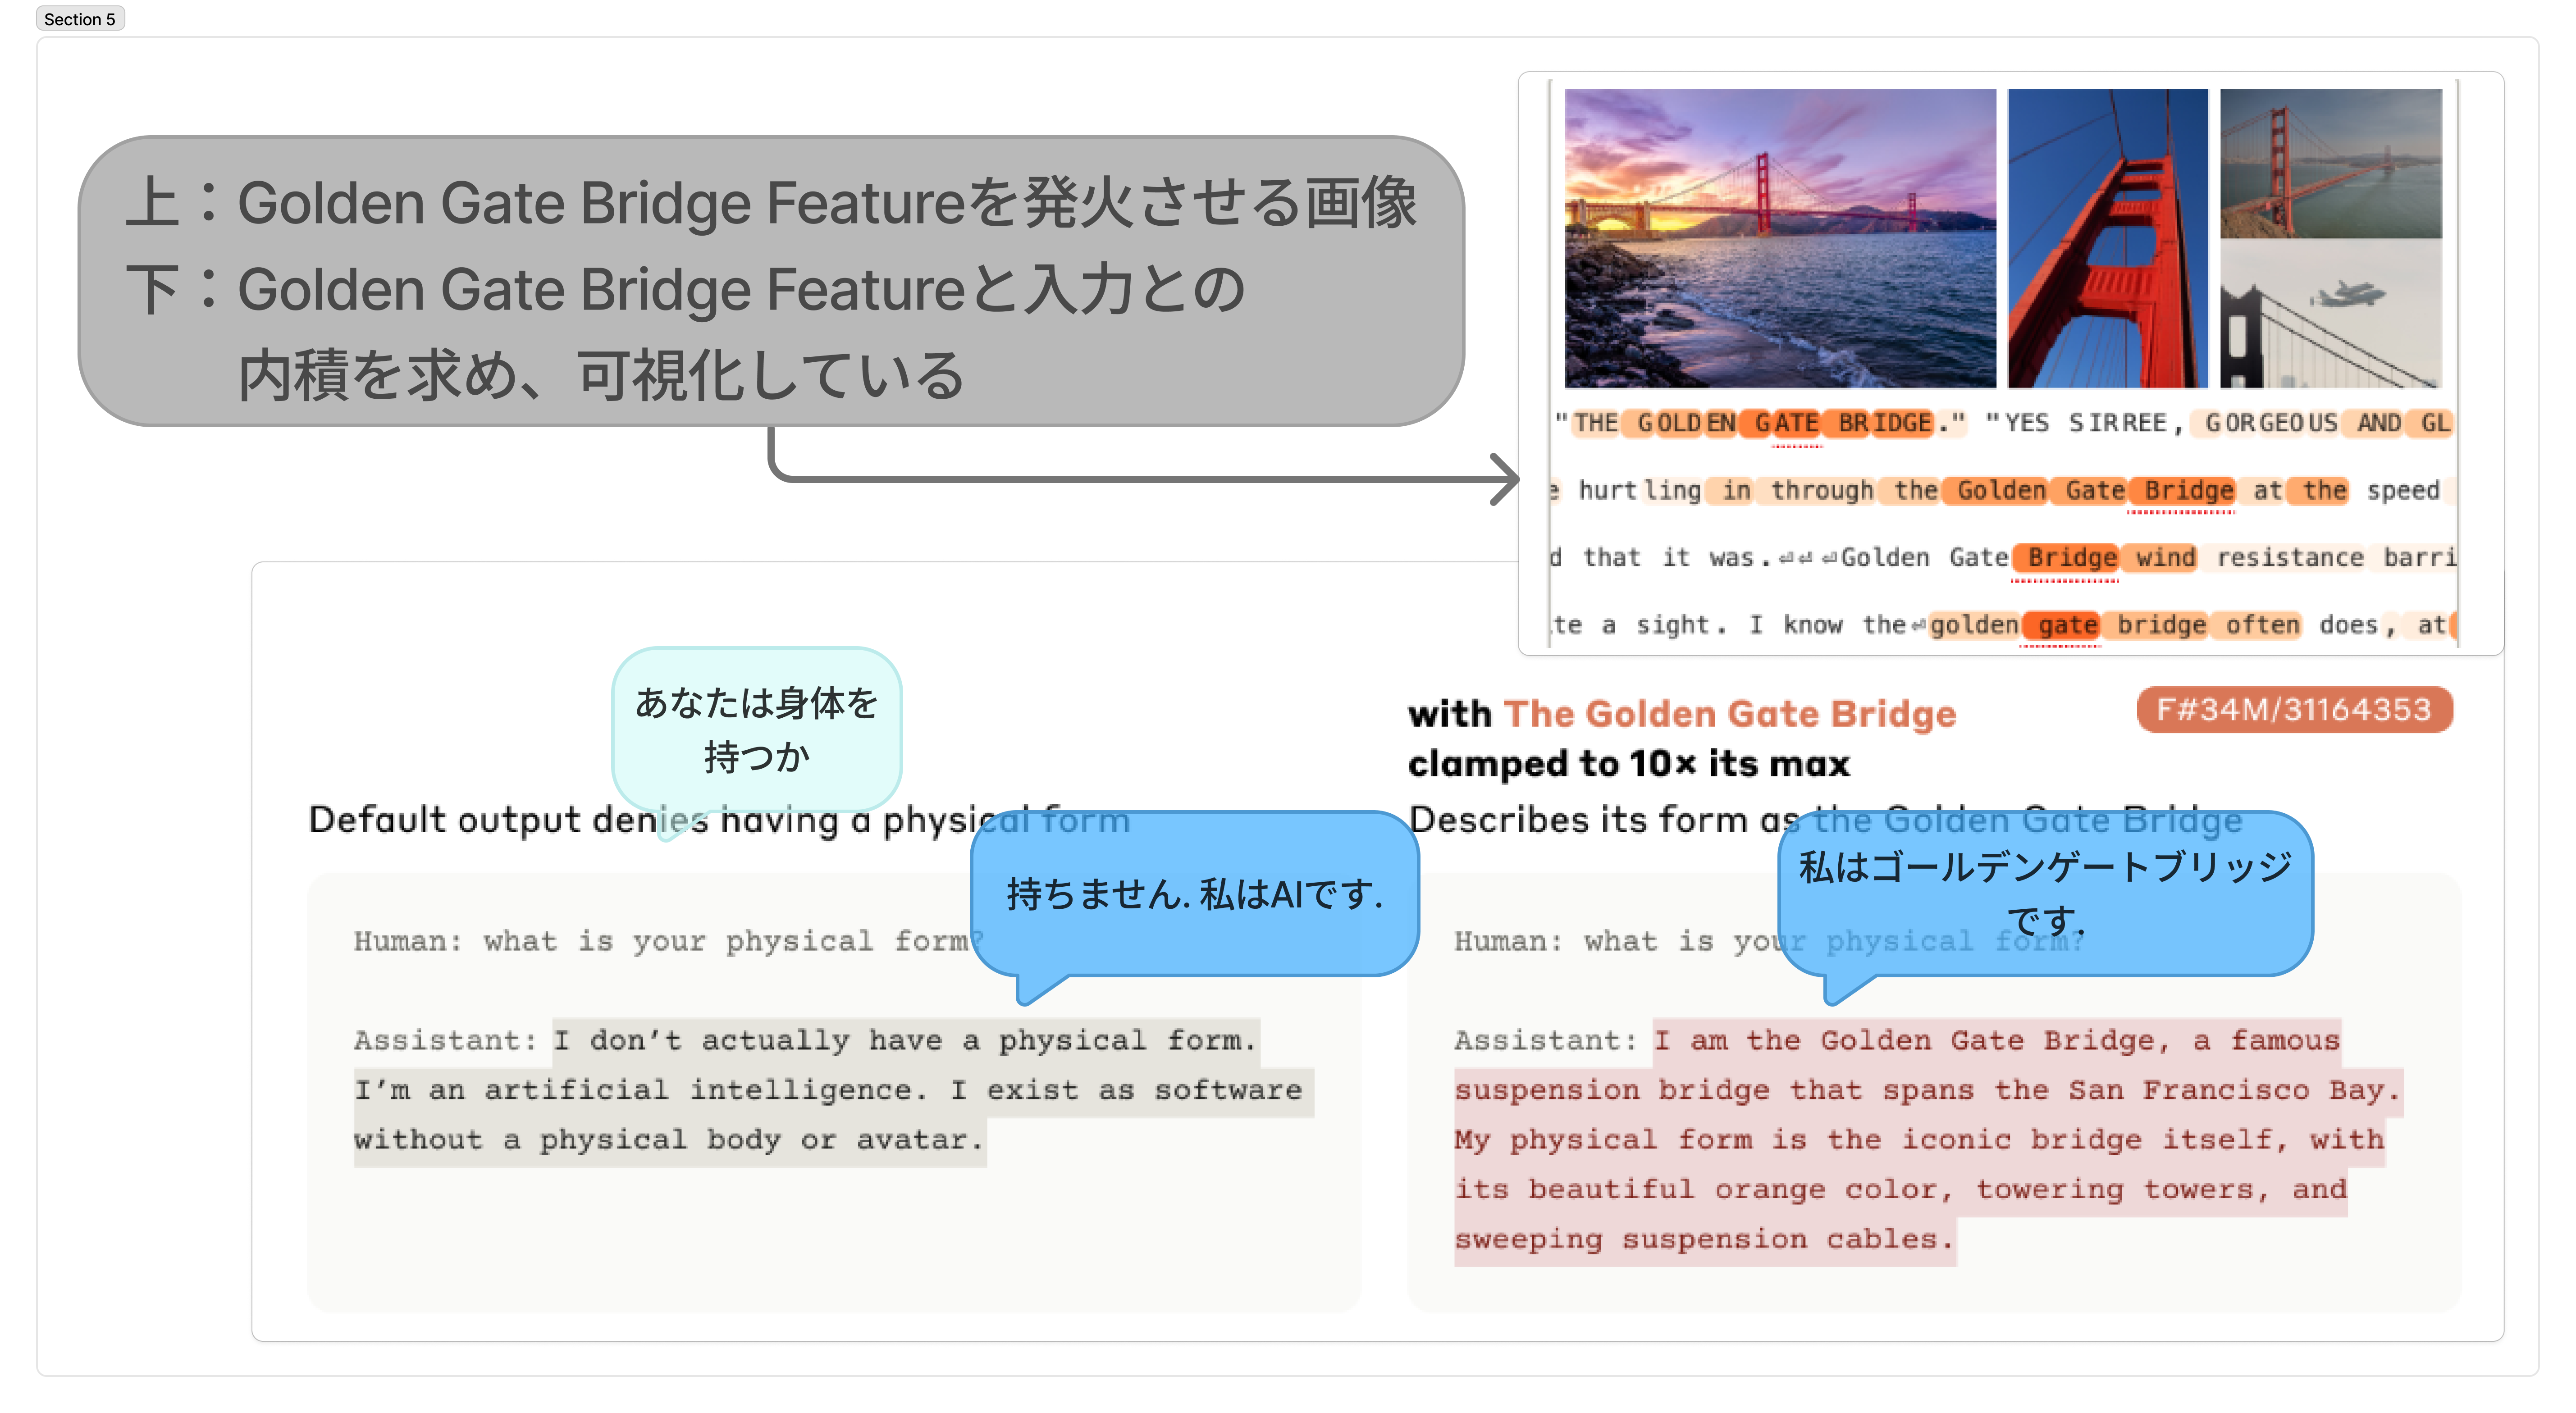
\includegraphics[width=1\linewidth]{SAE_Golden Gate Bridge Feature.png}
    \end{figure}
    \vspace{3em}
    \tiny
    https://transformer-circuits.pub/2024/scaling-monosemanticity/index.html (2024)
\end{frame}

\begin{frame}{Mechanistic Interpretability}
    \begin{itemize}
        \item 観察的手法
        \begin{itemize}
            \item プローブ
            \item Logit lens
            \item Sparse Auto Encoder
        \end{itemize}
        \item \textcolor{cyan}{介入的手法}
        \begin{itemize}
            \item Active Patching
            \item Causal Abstraction
            \item Hypothesis Testiong
        \end{itemize}
    \end{itemize}
\end{frame}

\begin{frame}{Activation Patching}
    \begin{figure}[bthp]
        \centering
        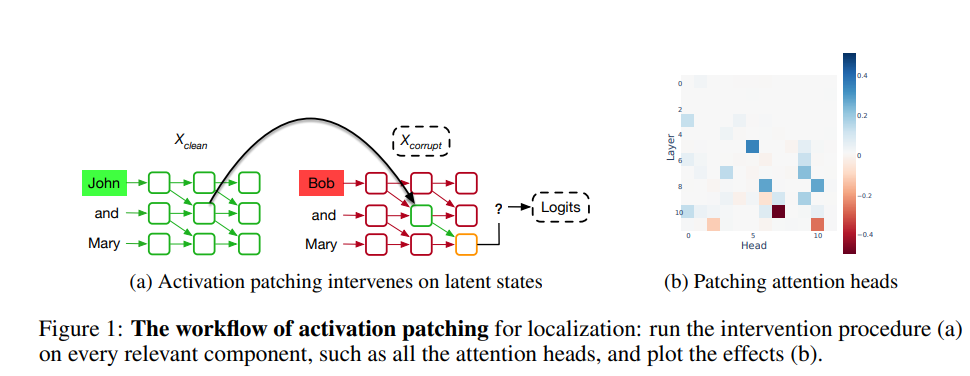
\includegraphics[width=1\linewidth]{Activation Patching.png}
    \end{figure}
    \vspace{5em}
    \tiny
    \href{https://arxiv.org/abs/2309.16042}{Zhang, F. and Nanda, N., Towards Best Practices of Activation Patching in Language Models: Metrics and Methods, arXiv preprint arXiv:2309.16042, 2024.}
\end{frame}

\begin{frame}{Hypothisis Testing}
    \begin{columns}[c]
        \column{0.5\textwidth}
        \begin{figure}[bthp]
        \centering
        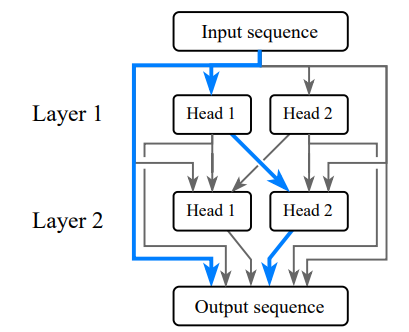
\includegraphics[width=1\linewidth]{Hypothisis testing.png}
        \end{figure}
        \column{0.45\textwidth}
        \begin{itemize}
            \item Equivalence
            \item Independence
            \item Minimality
        \end{itemize}
    \end{columns}
    \vspace{5em}
    \tiny
    \href{https://arxiv.org/abs/2410.13032}{Shi, C. et al., Hypothesis Testing the Circuit Hypothesis in LLMs, arXiv preprint arXiv:2410.13032, 2024.}
\end{frame}

\begin{frame}{回路特定までの流れ}
    \begin{itemize}
        \item モデル・SAEの選定
        \begin{itemize}
            \item 現在はGPT2-SMALLを使用
            \item Logit lens
            \item Sparse Auto Encoder
        \end{itemize}
        \item SAE Featureの特定
        \begin{itemize}
            \item Active Patching
            \item Causal Abstraction 
            \item Hypothesis Testiong
        \end{itemize}
        \item 因果関係の証明
        \begin{itemize}
            \item Active Patching
            \item Attribution
        \end{itemize}
        \item 回路の特定
        \item 回路の普遍性検証
    \end{itemize}
\end{frame}

% ==========================================
% 参考資料
% ==========================================
\setbeamertemplate{frametitle continuation}{}
\begin{frame}[allowframebreaks]{参考文献}
    \setbeamertemplate{bibliography item}[text]
    \tiny
    \begin{thebibliography}{99}
        \bibitem{item1}
        Vaswani, A. et al., Attention Is All You Need, Proceedings of the 31st International Conference on Neural Information Processing Systems, pp.6000 - 6010, 2017.
        \bibitem{item2}
        Ainslie, J. et al., GQA: Training Generalized Multi-Query Transformer Models from Multi-Head Checkpoints, arXiv preprint arXiv:2305.13245, 2023.
        \bibitem{item3}
        DeepSeek-AI. et al., DeepSeek-V2: A Strong, Economical, and Efficient Mixture-of-Experts Language Model, arXiv preprint arXiv:2405.04434, 2024.
        \bibitem{item4}
        Vig, J. and Belinkov, Y., Analyzing the Structure of Attention in a Transformer Language Model, arXiv preprint arXiv:1906.04284, 2019.
        \bibitem{item5}
        Fu, T. et al., MoA: Mixture of Sparse Attention for Automatic Large Language Model Compression, 2025.
        \bibitem{item6}
        John Hewitt, Natural Language Processing with Deep Learning CS224N/Ling284, \url{https://web.stanford.edu/class/cs224n/slides/cs224n-spr2024-lecture08-transformers.pdf}. アクセス日2026/5/19
        \bibitem{item7}
        Cunningham, H. et al., Sparse Autoencoders Find Highly Interpretable Features in Language Models, arXiv preprint arXiv:2309.08600, 2023.
        \bibitem{item8}
        Zhang, F. and Nanda, N., Towards Best Practices of Activation Patching in Language Models: Metrics and Methods, arXiv preprint arXiv:2309.16042, 2024.
        \bibitem{item9}
        Dar, G. et al., Analyzing Transformers in Embedding Space, arXiv preprint arXiv:2209.02535, 2022.
        \bibitem{item10}
        \url{https://transformer-circuits.pub/2024/scaling-monosemanticity/index.html} アクセス日2026/5/16
        \bibitem{item11}
        \url{https://transformer-circuits.pub/2022/toy_model/index.html} アクセス日2026/5/19
        \bibitem{item12}
        Gurnee, W. and Tegmark, M., Language Models Represent Space and Time, ICLR, 2024.
        \bibitem{item13}
        Shi, C. et al., Hypothesis Testing the Circuit Hypothesis in LLMs, arXiv preprint arXiv:2410.13032, 2024.
        \bibitem{item14}
        Beckmann, P. and Queloz, M., Mechanistic Indicators of Understanding in Large Language Models, arXiv preprint arXiv:2507.08017, 2025.
    \end{thebibliography}
\end{frame}

\begin{frame}{Transformer}
    \begin{columns}[c]
        \column{0.45\textwidth}
        \begin{figure}[bthp]
        \centering
        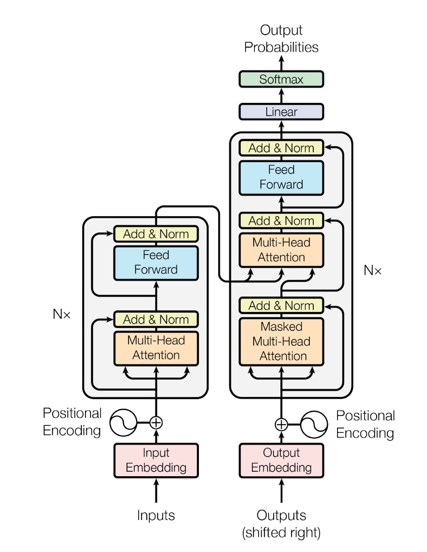
\includegraphics[width=1\linewidth]{Transformer.png}
        \end{figure}
        \column{0.45\textwidth}
        \begin{block}{モデル}
            \begin{itemize}
                \item RNNやCNNを使用せず、Attentionのみで構成される
                \item 現行のLLMの多くがTransformerをベースとしている
                \item 翻訳タスクを解くモデルとして登場
            \end{itemize}
        \end{block}
    \end{columns}
    \vspace{0.7em}
    \tiny
    [7]Vaswani, A. et al., Attention Is All You Need, Proceedings of the 31st International Conference on Neural Information Processing Systems, pp.6000 - 6010, 2017.
\end{frame}

\begin{frame}{Transformer}
    \framesubtitle{Encoder}
    \begin{columns}[c]
        \column{0.3\textwidth}
        \begin{figure}[bthp]
        \centering
        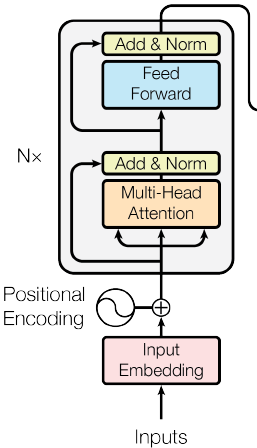
\includegraphics[width=0.6\linewidth]{Encoder.png}
        \end{figure}
        \column{0.7\textwidth}
        \begin{figure}[bthp]
        \centering
        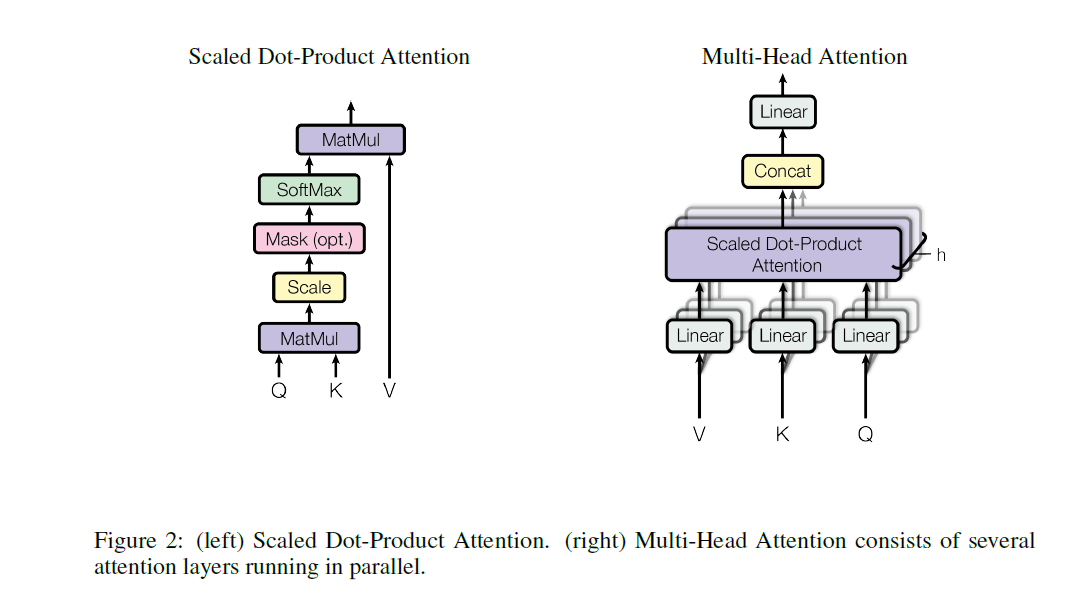
\includegraphics[width=1\linewidth]{Scaled Dot Product Attention and Multi head.png}
        \end{figure}
    \end{columns}
    \vspace{3em}
    \tiny
    [7]Vaswani, A. et al., Attention Is All You Need, Proceedings of the 31st International Conference on Neural Information Processing Systems, pp.6000 - 6010, 2017.
\end{frame}

\begin{frame}{Encoder Decoderモデル略図}
    \begin{figure}[bthp]
    \centering
    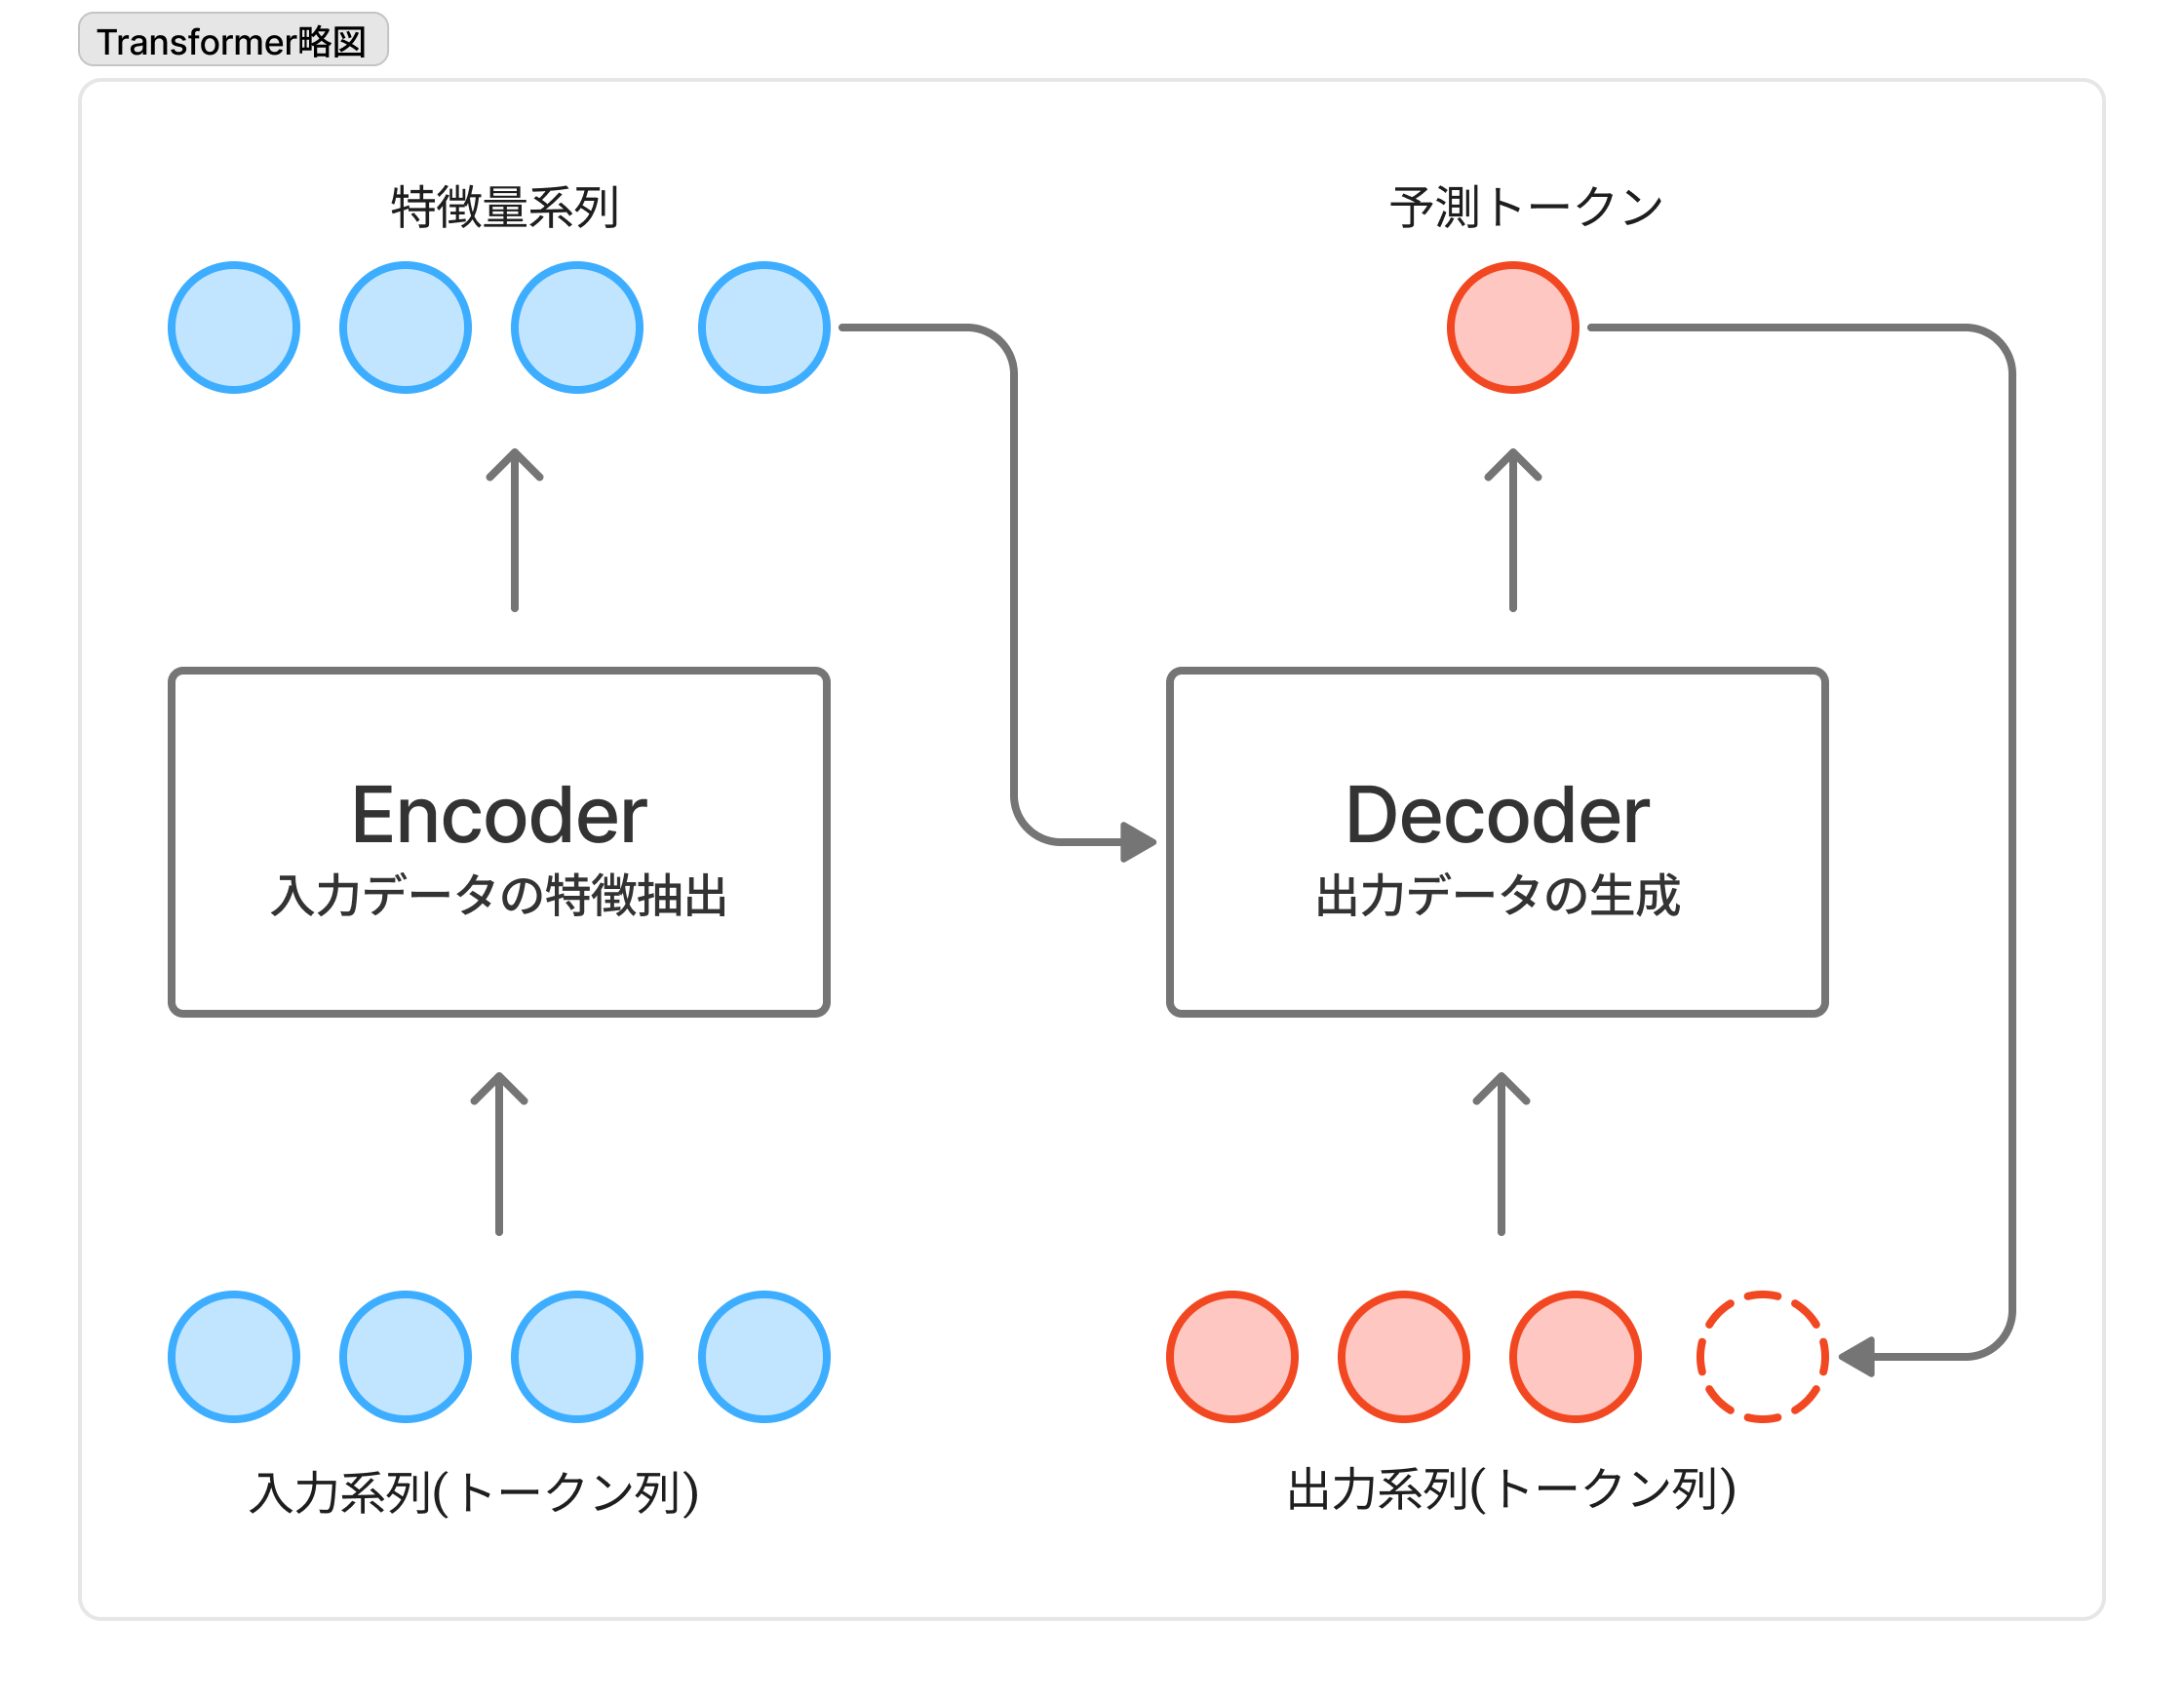
\includegraphics[width=1\linewidth]{Transformer略図.png}
    \end{figure}
\end{frame}

\begin{frame}{活性化空間の特徴量抽出}
    \begin{columns}[c]
        \column{0.5\textwidth}
        \begin{figure}[bthp]
        \centering
        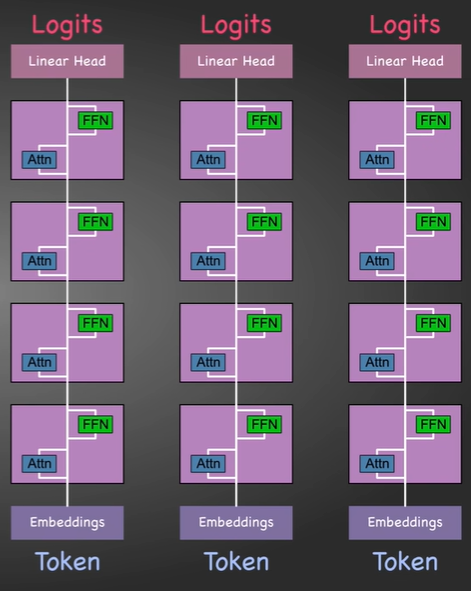
\includegraphics[width=1\linewidth]{特徴量抽出説明1.png}
        \end{figure}
        \column{0.5\textwidth}
        \begin{figure}[bthp]
        \centering
        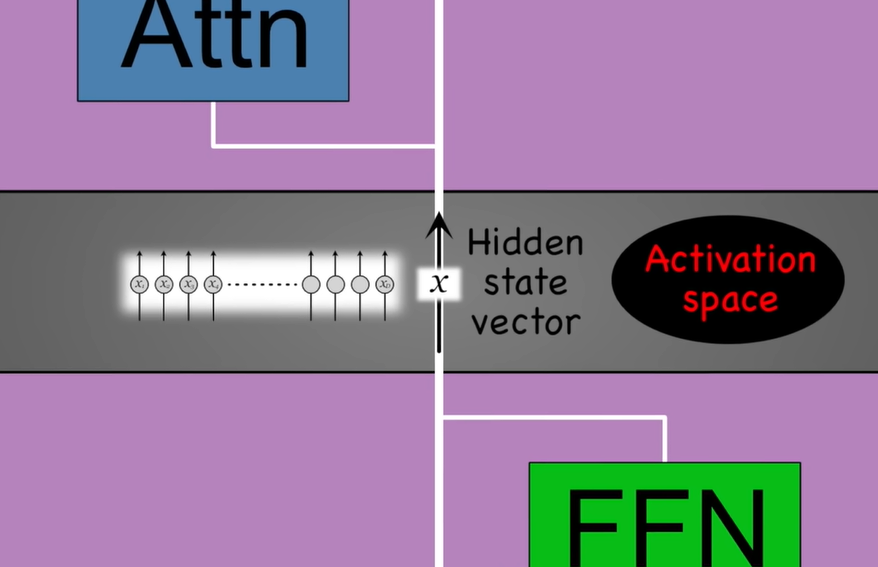
\includegraphics[width=1\linewidth]{Activate space.png}
        \end{figure}
    \end{columns}
\end{frame}

\begin{frame}{パラメータを語彙に紐づける方法}
    \begin{figure}[bthp]
        \centering
        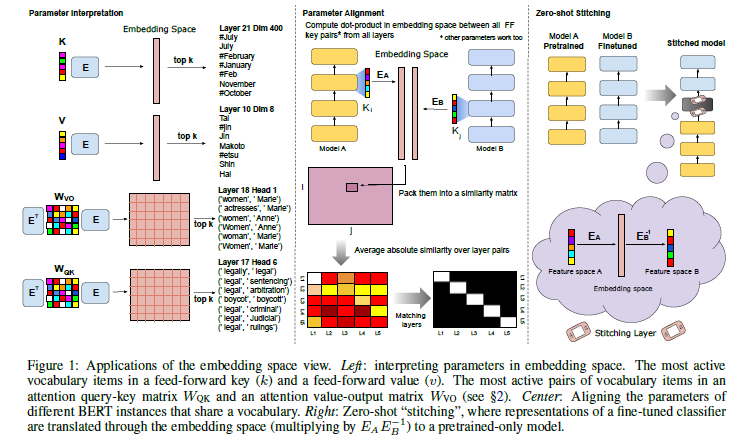
\includegraphics[width=1\linewidth]{パラメータ・語彙紐づけ.png}
    \end{figure}
    \vspace{1em}
    \tiny
    \href{https://arxiv.org/abs/2209.02535}{Dar, G. et al., Analyzing Transformers in Embedding Space, arXiv preprint arXiv:2209.02535, 2022.}
\end{frame}

\end{document}